% Generated by Sphinx.
\def\sphinxdocclass{report}
\documentclass[a4paper,12pt,spanish]{sphinxmanual}
\usepackage[utf8]{inputenc}
\DeclareUnicodeCharacter{00A0}{\nobreakspace}
\usepackage{cmap}
\usepackage[T1]{fontenc}
\usepackage{babel}
\usepackage{times}
\usepackage[Sonny]{fncychap}
\usepackage{longtable}
\usepackage{sphinx}
\usepackage{multirow}

\addto\captionsspanish{\renewcommand{\figurename}{Figura }}
\addto\captionsspanish{\renewcommand{\tablename}{Tabla }}
\floatname{literal-block}{Lista }


  \setcounter{tocdepth}{2}
  \fancypagestyle{normal}{
    \fancyhf{}
    % Footer

    \fancyfoot[LE,RO]{{\textbf{\textsf{\thepage}}}}
    \fancyfoot[LO]{{\sffamily\bfseries\nouppercase{\textbf{\rightmark}}}}
    \fancyfoot[RE]{{\sffamily\bfseries\nouppercase{\textbf{\leftmark}}}}

    \fancyhead[LE,RO]{{\sffamily\bfseries\nouppercase{\textit{Introducción al desarrollo de software}}}}

    \renewcommand{\headrulewidth}{0.4pt}
    \renewcommand{\footrulewidth}{0.4pt}
  }
  % Update the plain style so we get the page number & footer line,
  % but not a chapter or section title.  This is to keep the first
  % page of a chapter and the blank page between chapters `clean.'
  \fancypagestyle{plain}{
    \fancyhf{}
    \fancyfoot[RO,RE]{{\textbf{\textsf{\thepage}}}}
    \renewcommand{\headrulewidth}{0pt}
    \renewcommand{\footrulewidth}{0.4pt}
  }


\title{Introducción al desarrollo de software}
\date{15 de September de 2015}
\release{1.0}
\author{Emiliano López}
\newcommand{\sphinxlogo}{}
\renewcommand{\releasename}{Publicación}
\makeindex

\makeatletter
\def\PYG@reset{\let\PYG@it=\relax \let\PYG@bf=\relax%
    \let\PYG@ul=\relax \let\PYG@tc=\relax%
    \let\PYG@bc=\relax \let\PYG@ff=\relax}
\def\PYG@tok#1{\csname PYG@tok@#1\endcsname}
\def\PYG@toks#1+{\ifx\relax#1\empty\else%
    \PYG@tok{#1}\expandafter\PYG@toks\fi}
\def\PYG@do#1{\PYG@bc{\PYG@tc{\PYG@ul{%
    \PYG@it{\PYG@bf{\PYG@ff{#1}}}}}}}
\def\PYG#1#2{\PYG@reset\PYG@toks#1+\relax+\PYG@do{#2}}

\expandafter\def\csname PYG@tok@gd\endcsname{\def\PYG@tc##1{\textcolor[rgb]{0.63,0.00,0.00}{##1}}}
\expandafter\def\csname PYG@tok@gu\endcsname{\let\PYG@bf=\textbf\def\PYG@tc##1{\textcolor[rgb]{0.50,0.00,0.50}{##1}}}
\expandafter\def\csname PYG@tok@gt\endcsname{\def\PYG@tc##1{\textcolor[rgb]{0.00,0.27,0.87}{##1}}}
\expandafter\def\csname PYG@tok@gs\endcsname{\let\PYG@bf=\textbf}
\expandafter\def\csname PYG@tok@gr\endcsname{\def\PYG@tc##1{\textcolor[rgb]{1.00,0.00,0.00}{##1}}}
\expandafter\def\csname PYG@tok@cm\endcsname{\let\PYG@it=\textit\def\PYG@tc##1{\textcolor[rgb]{0.25,0.50,0.56}{##1}}}
\expandafter\def\csname PYG@tok@vg\endcsname{\def\PYG@tc##1{\textcolor[rgb]{0.73,0.38,0.84}{##1}}}
\expandafter\def\csname PYG@tok@m\endcsname{\def\PYG@tc##1{\textcolor[rgb]{0.13,0.50,0.31}{##1}}}
\expandafter\def\csname PYG@tok@mh\endcsname{\def\PYG@tc##1{\textcolor[rgb]{0.13,0.50,0.31}{##1}}}
\expandafter\def\csname PYG@tok@cs\endcsname{\def\PYG@tc##1{\textcolor[rgb]{0.25,0.50,0.56}{##1}}\def\PYG@bc##1{\setlength{\fboxsep}{0pt}\colorbox[rgb]{1.00,0.94,0.94}{\strut ##1}}}
\expandafter\def\csname PYG@tok@ge\endcsname{\let\PYG@it=\textit}
\expandafter\def\csname PYG@tok@vc\endcsname{\def\PYG@tc##1{\textcolor[rgb]{0.73,0.38,0.84}{##1}}}
\expandafter\def\csname PYG@tok@il\endcsname{\def\PYG@tc##1{\textcolor[rgb]{0.13,0.50,0.31}{##1}}}
\expandafter\def\csname PYG@tok@go\endcsname{\def\PYG@tc##1{\textcolor[rgb]{0.20,0.20,0.20}{##1}}}
\expandafter\def\csname PYG@tok@cp\endcsname{\def\PYG@tc##1{\textcolor[rgb]{0.00,0.44,0.13}{##1}}}
\expandafter\def\csname PYG@tok@gi\endcsname{\def\PYG@tc##1{\textcolor[rgb]{0.00,0.63,0.00}{##1}}}
\expandafter\def\csname PYG@tok@gh\endcsname{\let\PYG@bf=\textbf\def\PYG@tc##1{\textcolor[rgb]{0.00,0.00,0.50}{##1}}}
\expandafter\def\csname PYG@tok@ni\endcsname{\let\PYG@bf=\textbf\def\PYG@tc##1{\textcolor[rgb]{0.84,0.33,0.22}{##1}}}
\expandafter\def\csname PYG@tok@nl\endcsname{\let\PYG@bf=\textbf\def\PYG@tc##1{\textcolor[rgb]{0.00,0.13,0.44}{##1}}}
\expandafter\def\csname PYG@tok@nn\endcsname{\let\PYG@bf=\textbf\def\PYG@tc##1{\textcolor[rgb]{0.05,0.52,0.71}{##1}}}
\expandafter\def\csname PYG@tok@no\endcsname{\def\PYG@tc##1{\textcolor[rgb]{0.38,0.68,0.84}{##1}}}
\expandafter\def\csname PYG@tok@na\endcsname{\def\PYG@tc##1{\textcolor[rgb]{0.25,0.44,0.63}{##1}}}
\expandafter\def\csname PYG@tok@nb\endcsname{\def\PYG@tc##1{\textcolor[rgb]{0.00,0.44,0.13}{##1}}}
\expandafter\def\csname PYG@tok@nc\endcsname{\let\PYG@bf=\textbf\def\PYG@tc##1{\textcolor[rgb]{0.05,0.52,0.71}{##1}}}
\expandafter\def\csname PYG@tok@nd\endcsname{\let\PYG@bf=\textbf\def\PYG@tc##1{\textcolor[rgb]{0.33,0.33,0.33}{##1}}}
\expandafter\def\csname PYG@tok@ne\endcsname{\def\PYG@tc##1{\textcolor[rgb]{0.00,0.44,0.13}{##1}}}
\expandafter\def\csname PYG@tok@nf\endcsname{\def\PYG@tc##1{\textcolor[rgb]{0.02,0.16,0.49}{##1}}}
\expandafter\def\csname PYG@tok@si\endcsname{\let\PYG@it=\textit\def\PYG@tc##1{\textcolor[rgb]{0.44,0.63,0.82}{##1}}}
\expandafter\def\csname PYG@tok@s2\endcsname{\def\PYG@tc##1{\textcolor[rgb]{0.25,0.44,0.63}{##1}}}
\expandafter\def\csname PYG@tok@vi\endcsname{\def\PYG@tc##1{\textcolor[rgb]{0.73,0.38,0.84}{##1}}}
\expandafter\def\csname PYG@tok@nt\endcsname{\let\PYG@bf=\textbf\def\PYG@tc##1{\textcolor[rgb]{0.02,0.16,0.45}{##1}}}
\expandafter\def\csname PYG@tok@nv\endcsname{\def\PYG@tc##1{\textcolor[rgb]{0.73,0.38,0.84}{##1}}}
\expandafter\def\csname PYG@tok@s1\endcsname{\def\PYG@tc##1{\textcolor[rgb]{0.25,0.44,0.63}{##1}}}
\expandafter\def\csname PYG@tok@gp\endcsname{\let\PYG@bf=\textbf\def\PYG@tc##1{\textcolor[rgb]{0.78,0.36,0.04}{##1}}}
\expandafter\def\csname PYG@tok@sh\endcsname{\def\PYG@tc##1{\textcolor[rgb]{0.25,0.44,0.63}{##1}}}
\expandafter\def\csname PYG@tok@ow\endcsname{\let\PYG@bf=\textbf\def\PYG@tc##1{\textcolor[rgb]{0.00,0.44,0.13}{##1}}}
\expandafter\def\csname PYG@tok@sx\endcsname{\def\PYG@tc##1{\textcolor[rgb]{0.78,0.36,0.04}{##1}}}
\expandafter\def\csname PYG@tok@bp\endcsname{\def\PYG@tc##1{\textcolor[rgb]{0.00,0.44,0.13}{##1}}}
\expandafter\def\csname PYG@tok@c1\endcsname{\let\PYG@it=\textit\def\PYG@tc##1{\textcolor[rgb]{0.25,0.50,0.56}{##1}}}
\expandafter\def\csname PYG@tok@kc\endcsname{\let\PYG@bf=\textbf\def\PYG@tc##1{\textcolor[rgb]{0.00,0.44,0.13}{##1}}}
\expandafter\def\csname PYG@tok@c\endcsname{\let\PYG@it=\textit\def\PYG@tc##1{\textcolor[rgb]{0.25,0.50,0.56}{##1}}}
\expandafter\def\csname PYG@tok@mf\endcsname{\def\PYG@tc##1{\textcolor[rgb]{0.13,0.50,0.31}{##1}}}
\expandafter\def\csname PYG@tok@err\endcsname{\def\PYG@bc##1{\setlength{\fboxsep}{0pt}\fcolorbox[rgb]{1.00,0.00,0.00}{1,1,1}{\strut ##1}}}
\expandafter\def\csname PYG@tok@mb\endcsname{\def\PYG@tc##1{\textcolor[rgb]{0.13,0.50,0.31}{##1}}}
\expandafter\def\csname PYG@tok@ss\endcsname{\def\PYG@tc##1{\textcolor[rgb]{0.32,0.47,0.09}{##1}}}
\expandafter\def\csname PYG@tok@sr\endcsname{\def\PYG@tc##1{\textcolor[rgb]{0.14,0.33,0.53}{##1}}}
\expandafter\def\csname PYG@tok@mo\endcsname{\def\PYG@tc##1{\textcolor[rgb]{0.13,0.50,0.31}{##1}}}
\expandafter\def\csname PYG@tok@kd\endcsname{\let\PYG@bf=\textbf\def\PYG@tc##1{\textcolor[rgb]{0.00,0.44,0.13}{##1}}}
\expandafter\def\csname PYG@tok@mi\endcsname{\def\PYG@tc##1{\textcolor[rgb]{0.13,0.50,0.31}{##1}}}
\expandafter\def\csname PYG@tok@kn\endcsname{\let\PYG@bf=\textbf\def\PYG@tc##1{\textcolor[rgb]{0.00,0.44,0.13}{##1}}}
\expandafter\def\csname PYG@tok@o\endcsname{\def\PYG@tc##1{\textcolor[rgb]{0.40,0.40,0.40}{##1}}}
\expandafter\def\csname PYG@tok@kr\endcsname{\let\PYG@bf=\textbf\def\PYG@tc##1{\textcolor[rgb]{0.00,0.44,0.13}{##1}}}
\expandafter\def\csname PYG@tok@s\endcsname{\def\PYG@tc##1{\textcolor[rgb]{0.25,0.44,0.63}{##1}}}
\expandafter\def\csname PYG@tok@kp\endcsname{\def\PYG@tc##1{\textcolor[rgb]{0.00,0.44,0.13}{##1}}}
\expandafter\def\csname PYG@tok@w\endcsname{\def\PYG@tc##1{\textcolor[rgb]{0.73,0.73,0.73}{##1}}}
\expandafter\def\csname PYG@tok@kt\endcsname{\def\PYG@tc##1{\textcolor[rgb]{0.56,0.13,0.00}{##1}}}
\expandafter\def\csname PYG@tok@sc\endcsname{\def\PYG@tc##1{\textcolor[rgb]{0.25,0.44,0.63}{##1}}}
\expandafter\def\csname PYG@tok@sb\endcsname{\def\PYG@tc##1{\textcolor[rgb]{0.25,0.44,0.63}{##1}}}
\expandafter\def\csname PYG@tok@k\endcsname{\let\PYG@bf=\textbf\def\PYG@tc##1{\textcolor[rgb]{0.00,0.44,0.13}{##1}}}
\expandafter\def\csname PYG@tok@se\endcsname{\let\PYG@bf=\textbf\def\PYG@tc##1{\textcolor[rgb]{0.25,0.44,0.63}{##1}}}
\expandafter\def\csname PYG@tok@sd\endcsname{\let\PYG@it=\textit\def\PYG@tc##1{\textcolor[rgb]{0.25,0.44,0.63}{##1}}}

\def\PYGZbs{\char`\\}
\def\PYGZus{\char`\_}
\def\PYGZob{\char`\{}
\def\PYGZcb{\char`\}}
\def\PYGZca{\char`\^}
\def\PYGZam{\char`\&}
\def\PYGZlt{\char`\<}
\def\PYGZgt{\char`\>}
\def\PYGZsh{\char`\#}
\def\PYGZpc{\char`\%}
\def\PYGZdl{\char`\$}
\def\PYGZhy{\char`\-}
\def\PYGZsq{\char`\'}
\def\PYGZdq{\char`\"}
\def\PYGZti{\char`\~}
% for compatibility with earlier versions
\def\PYGZat{@}
\def\PYGZlb{[}
\def\PYGZrb{]}
\makeatother

\renewcommand\PYGZsq{\textquotesingle}

\begin{document}
\shorthandoff{"}

\begin{titlepage}%
    \let\footnotesize\small
    \let\footnoterule\relax
    \rule{\textwidth}{1pt}%
    \begin{flushright}%
      \sphinxlogo%
      \vspace{15 mm}
      {\rm\Huge Introducción al desarrollo de software\\ }
      {\em\large Tecnicatura Universitaria en Software Libre}
      \vfill
      {
        \begin{tabular}[t]{c}
          \large Emiliano P. López \\
          \large Maximiliano Boscovich
        \end{tabular}
        \par}
      \vfill\vfill
      {\large
        Mayo de 2015
       \vfill
       UNIVERSIDAD NACIONAL DEL LITORAL\\
          Facutlad de Ingeniería y Ciencias Hídricas\\
      }%
    \end{flushright}%\par
  \end{titlepage}%
  %\vspace{\fill}
  %\includegraphics{cc.png}
  \cleardoublepage%
  \phantomsection\label{pre:dedication}
  \vspace*{\fill}
  \begin{flushright}
    \emph{A todos los que están mirando,\\por el amor}
  \end{flushright}
  \vspace{\fill}

\tableofcontents
\phantomsection\label{index::doc}


Contents:

Tabla de Contenidos

\begin{Verbatim}[commandchars=\\\{\}]
\PYGZpc{}\PYGZpc{}javascript
\PYGZdl{}.getScript(\PYGZsq{}https://kmahelona.github.io/ipython\PYGZus{}notebook\PYGZus{}goodies/ipython\PYGZus{}notebook\PYGZus{}toc.js\PYGZsq{})
\end{Verbatim}

\begin{Verbatim}[commandchars=\\\{\}]
\PYGZlt{}IPython.core.display.Javascript object\PYGZgt{}
\end{Verbatim}


\chapter{Introducción}
\label{Unidad01:introduccion}\label{Unidad01::doc}\label{Unidad01:introduccion-al-desarrollo-de-software}
En el presente capítulo introduciremos los conceptos necesarios para
desarrollar los primeros algoritmos computacionales. Además, se explican
las herramientas necesarias para llevar a cabo el desarrollo y sus
diferentes alternativas.


\section{Motivación}
\label{Unidad01:motivacion}
Gran parte de las tecnologías utilizadas en la actualidad tienen algo en
común, y es que por lo general basan su lógica en algún tipo de
programa. Saber programar nos permite comprender su funcionamiento y con
esto nos abre un gran abanico de posibilidades, limitadas únicamente por
nuestra imaginación. Pensemos por un momento en todas las aplicaciones
que usamos a diario en el teléfono celular, en la PC, en la tablet, etc.
Saber que si necesitamos algo en concreto seremos capaces de crearlo
nosotros mismos es pura libertad.

Lo más importante de todo, es que no es necesario ser un genio para
poder programar, simplemente tenemos que aprender un conjunto de reglas
básicas, saber como aplicarlas y tener muchas ganas de crear cosas
nuevas. Además, programar es muy divertido, al contrario de lo que mucha
gente podría pensar en un principio. Es como un gran rompecabezas en el
que debemos encajar ciertas piezas de una forma específica para
conseguir el resultado deseado.

A lo largo de esta materia utilizaremos como lenguaje de programación a
Python (\href{http://www.python.org}{http://www.python.org}).


\subsection{¿Por qué Python?}
\label{Unidad01:por-que-python}
\begin{DUlineblock}{0em}
\item[] Python es un lenguaje de programación multiproposito, poderoso y fácil
\end{DUlineblock}

de aprender. Es del tipo interpretado, lo que quiere decir que los
programas realizados con python no necesitan ser compilados, en su
lugar, simplemente requieren que el equipo donde van a ser ejecutados
cuente con un interprete de python instalado. Es un lenguaje que cuenta
con estructuras de datos eficientes y de alto nivel. Su elegante
sintaxis y su tipado dinámico hacen de éste un lenguaje ideal para el
desarrollo rápido de aplicaciones en diversas áreas como ser: *
Aplicaciones WEB * Aplicaciones científicas * Gráficas * Multimedia
* Juegos
\textbar{} * Etc.

Otra de las grandes virtudes de python, es que su interprete puede
ejecutarse en la mayoría de los sistemas operativos utilizados en la
actualidad (GNU/Linux, Microsoft Windows, Mac OSX, etc.).

Dada su versatilidad y simplicidad, Python es utilizado por companías
como Google, Youtube, Netflix, Yahoo, NSA, NASA, Canonical, IBM, entre
otras tantas.


\section{Instalando Python}
\label{Unidad01:instalando-python}
Actualmente existen dos versiones de Python comúnmente utilizadas, la
versión 2 y 3, ambas son completamente funcionales y muy utilizadas. En
este curso nos basaremos en la versión 3.

\textbf{Ver como funcionaría miniconda en windows y linux:}
\href{http://conda.pydata.org/miniconda.html}{http://conda.pydata.org/miniconda.html}


\subsection{Windows}
\label{Unidad01:windows}
Para instalar Python en una máquina con Windows, debemos seguir los
siguientes pasos:
\begin{itemize}
\item {} 
Apuntar el navegador a: \href{https://www.python.org/downloads/windows/}{https://www.python.org/downloads/windows/}

\item {} 
Ir al link de la última versión disponible (por ej: latest python 3
relase)

\item {} 
En la sección Files, descargar el instalador correspondiente a su
arquitectura (64/32 bits), por ej:
\href{https://www.python.org/ftp/python/3.4.3/python-3.4.3.msi}{https://www.python.org/ftp/python/3.4.3/python-3.4.3.msi}

\item {} 
Ejecutar el instalador (por ej: python-3.4.3.msi) aceptando las
opciones por defecto

\end{itemize}


\subsection{GNU/Linux}
\label{Unidad01:gnu-linux}
En la mayoría de las distribuciones GNU/Linux, es muy probable que ya
contemos con el intérprete instalado, incluso en sus dos versiones. En
caso de no ser así, para instalarlo utilizando los administradores de
paquetes debemos ejecutar los siguientes comandos desde una terminal:

Para sistemas basados en Debian (como Ubuntu o sus derivados):

\begin{Verbatim}[commandchars=\\\{\}]
sudo apt\PYGZhy{}get install python3
\end{Verbatim}

Para sistemas que utilizan yum como sistema de paquetes (Fedora, CentOS,
RedHat)

\begin{Verbatim}[commandchars=\\\{\}]
sudo yum install *python*
\end{Verbatim}


\section{Entornos de programación}
\label{Unidad01:entornos-de-programacion}

\subsection{El intérprete interactivo}
\label{Unidad01:el-interprete-interactivo}
Ya con el intérprete de Python instalado, podemos comenzar a programar.
Si ejecutamos en una terminal \code{python3}, ingresaremos al intérprete en
modo interactivo y veremos una salida similar a la siguiente:

\begin{Verbatim}[commandchars=\\\{\}]
Python 3.4.2 (default, Oct  8 2014, 10:45:20)
[GCC 4.9.1] on linux
Type \PYGZdq{}help\PYGZdq{}, \PYGZdq{}copyright\PYGZdq{}, \PYGZdq{}credits\PYGZdq{} or \PYGZdq{}license\PYGZdq{} for more information.
\PYGZgt{}\PYGZgt{}\PYGZgt{}
\end{Verbatim}

Con esto, el interprete de python esta listo para empezar a interpretar
las instrucciones (las cuales llamaremos sentencias) que forman parte de
nuestro programa, por lo que podemos decir que ya estamos listos para
empezar a programar. Pero vayamos de lo más sencillo a lo más complejo,
y lo mejor para comenzar es realizando ciertos cálculos matemáticos
sencillos, y corroborando su resultado. Por ejemplo, escribamos lo
siguiente:

\begin{Verbatim}[commandchars=\\\{\}]
\PYG{g+gp}{\PYGZgt{}\PYGZgt{}\PYGZgt{} }\PYG{l+m+mi}{2}\PYG{o}{*}\PYG{l+m+mi}{5}
\PYG{g+go}{10}
\PYG{g+go}{\PYGZgt{}\PYGZgt{}\PYGZgt{}}
\end{Verbatim}

Como vemos, si ingresamos 2*5, le estamos diciendo al interprete de
python que debe realizar la multiplicación entre 2 y 5. El interprete
analiza la instrucción ingresada (2*5), y contesta con el resultado (10
en este caso).

Hagamos otros calculos para entrar en calor

\begin{Verbatim}[commandchars=\\\{\}]
\PYG{g+gp}{\PYGZgt{}\PYGZgt{}\PYGZgt{} }\PYG{l+m+mi}{2}\PYG{o}{*}\PYG{l+m+mi}{5}\PYG{o}{+}\PYG{l+m+mi}{10}
\PYG{g+go}{20}
\PYG{g+gp}{\PYGZgt{}\PYGZgt{}\PYGZgt{} }\PYG{o}{\PYGZhy{}}\PYG{l+m+mi}{3}\PYG{o}{*}\PYG{l+m+mi}{19}\PYG{o}{+}\PYG{l+m+mf}{3.1415}
\PYG{g+go}{\PYGZhy{}53.8585}
\PYG{g+gp}{\PYGZgt{}\PYGZgt{}\PYGZgt{} }\PYG{l+m+mi}{2}\PYG{o}{/}\PYG{l+m+mf}{10.0}
\PYG{g+go}{0.2}
\PYG{g+go}{\PYGZgt{}\PYGZgt{}\PYGZgt{}}
\end{Verbatim}


\subsection{IPython, el intérprete interactivo mejorado}
\label{Unidad01:ipython-el-interprete-interactivo-mejorado}
\href{http://ipython.org}{IPython}\footnote{http://ipython.org} es una interfaz mejorada del intérprete
nativo. Se lo puede utilizar en modo consola o a través de una interfaz
web. La instalación en sistemas basados en Debian GNU/Linux es similar a
la de python: \code{apt-get install ipython3}.

La ejecución de ipython desde una terminal nos arroja una pantalla
similar a la siguiente:

\begin{Verbatim}[commandchars=\\\{\}]
emiliano@pynandi:\PYGZti{} \PYGZdl{} ipython3
Python 3.4.2 (default, Oct  8 2014, 10:45:20)
Type \PYGZdq{}copyright\PYGZdq{}, \PYGZdq{}credits\PYGZdq{} or \PYGZdq{}license\PYGZdq{} for more information.

IPython 2.3.0 \PYGZhy{}\PYGZhy{} An enhanced Interactive Python.
?         \PYGZhy{}\PYGZgt{} Introduction and overview of IPython\PYGZsq{}s features.
\PYGZpc{}quickref \PYGZhy{}\PYGZgt{} Quick reference.
help      \PYGZhy{}\PYGZgt{} Python\PYGZsq{}s own help system.
object?   \PYGZhy{}\PYGZgt{} Details about \PYGZsq{}object\PYGZsq{}, use \PYGZsq{}object??\PYGZsq{} for extra details.

In [1]:
\end{Verbatim}

Otra alternativa muy interesante son los notebooks de ipython, una
interfaz que permite programar utilizando el navegador web como entorno.
No entraremos en detalle ya que posteriormente analizaremos su
funcionamiento. Se debe ejecutar en una terminal \code{ipython3 notebook} y
esto abrirá el navegador por defecto con el entorno cargado.


\subsection{Entorno integrado de desarrollo (IDE)}
\label{Unidad01:entorno-integrado-de-desarrollo-ide}
Un IDE es un entorno que nos facilita las tareas a la hora de programar.
Consiste en la integración de un editor de texto con características de
resaltado de sintaxis, autocompletado -entre otras-, y el intérprete de
Python. Existen cientos de entornos muy buenos, como por ejemplo
\href{https://github.com/spyder-ide/spyder}{Spyder}\footnote{https://github.com/spyder-ide/spyder},
\href{https://www.jetbrains.com/pycharm}{PyCharm}\footnote{https://www.jetbrains.com/pycharm} o
\href{http://ninja-ide.org}{Ninja-IDE}\footnote{http://ninja-ide.org}. Para el presente curso, nos
basaremos en Ninja-IDE, software libre que ha sido desarrollado por la
comunidad de Python Argentina, \href{http://python.org.ar}{PyAr}\footnote{http://python.org.ar}.
\begin{figure}[htbp]
\centering

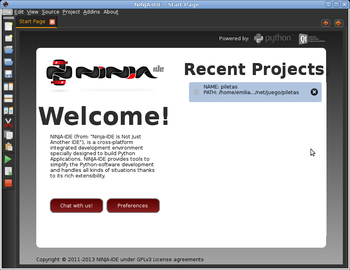
\includegraphics{files/img/u1/ninja-ide.png}
\end{figure}

Una lista bastante completa sobre las IDEs disponibles pueden
encontrarse en la \href{https://wiki.python.org/moin/IntegratedDevelopmentEnvironments}{wiki oficial de
Python}\footnote{https://wiki.python.org/moin/IntegratedDevelopmentEnvironments}


\section{Algoritmos computacionales}
\label{Unidad01:algoritmos-computacionales}
En forma simplificada, un programa o software es un conjunto de
instrucciones que la computadora puede ejecutar. Este procedimiento
formado por un conjunto de instrucciones es lo que denominamos algoritmo
computacional. Una analogía a un algoritmo computacional es una receta
de cocina, por ejemplo:

\begin{Verbatim}[commandchars=\\\{\}]
Prender el fuego
Salar la carne
Controlar cada 5 minutos hasta que haya brasas
Poner la carne a la parrilla
Cocinar hasta que esté la carne, controlar cada 5 minutos
Dar vuelta la carne
Cocinar hasta que esté la carne, controlar cada 5 minutos
Si falta sal al probar, salar
\end{Verbatim}

En esta receta se ven una serie de instrucciones que deben ser seguidas
en un determinado orden, en algunos casos contamos con ingredientes,
intrucciones, decisiones y acciones que se repiten. No muy distinto a un
programa de computación, comencemos con algunos \emph{ingredientes} simples
de Python y veamos lo que podemos hacer con ellos.


\subsection{El primer programa}
\label{Unidad01:el-primer-programa}
El acercamiento inicial a un lenguaje de programación suele ser con el
archiconocido programa ``Hola mundo''. Consiste simmplemente en un
programa que muestra en pantalla ese mensaje.

Renunciando a cualquier pretención de originalidad comenzaremos del
mismo modo, pero despidiéndonos. Para esto utilizaremos la instrucción
\emph{print()} pasando el mensaje de despedida entre comillas, a continuación
la instrucción.

\begin{Verbatim}[commandchars=\\\{\}]
\PYG{k}{print}\PYG{p}{(}\PYG{l+s}{\PYGZdq{}}\PYG{l+s}{Adios mundo cruel!}\PYG{l+s}{\PYGZdq{}}\PYG{p}{)}
\end{Verbatim}

Podemos probar la intrucción directamente desde el intérprete, creando
con un editor de texto plano un archivo guardado como \code{chau.py} y
luego ejecutándolo desde la terminal haciendo \code{python3 chau.py}, o
bien utilizando un IDE y haciendo todo desde ahí mismo.

Ahora bien, es muchísimo más lo que podemos hacer programando además de
saludar cordialmente. Veamos los elementos de un programa que nos
permitirán realizar tareas más complejas y entretenidas.


\section{Modos de ejecutar tus programas}
\label{Unidad01:modos-de-ejecutar-tus-programas}
El intérprete interactivo de Python es una gran ayuda para realizar
pruebas y experimentar en tiempo real sobre el lenguaje. Sin embargo,
cuando cerramos el intérprete perdemos lo escrito, por lo que no es una
solución para escribir programas mas largos y con mayores complejidades.
Por otro lado, tampoco resulta poco práctico abrir el IDE para correr un
script Python. Entonces, para un programa guardado con el nombre
hola\_mundo.py, lo podemos ejecutar de las siguientes maneras:


\subsection{Desde la línea de comandos}
\label{Unidad01:desde-la-linea-de-comandos}
Abriendo una terminal, e invocando al intérprete python y luego la ruta
y nombre del archivo:

\begin{Verbatim}[commandchars=\\\{\}]
\PYGZdl{}python3 hola\PYGZus{}mundo.py
\end{Verbatim}


\subsection{Como un script}
\label{Unidad01:como-un-script}
Es posible ejecutarlo sin invocar al intérprete desde la línea de
comandos, para esto, se debe incluir al principio del programa la
siguiente línea:

\begin{Verbatim}[commandchars=\\\{\}]
\PYG{c}{\PYGZsh{}!/usr/bin/env python3}
\end{Verbatim}

Con esa línea, estaremos especificando en el mismo programa la ruta del
intérprete que debe ejecutarlo. Antes de poder ejecutarlo, debemos
otorgarle permisos de ejecución con el comando del sistema operativo
chmod:

\begin{Verbatim}[commandchars=\\\{\}]
\PYGZdl{}chmod +x hola\PYGZus{}mundo.py
\end{Verbatim}

Una vez realizado lo anterior, es posible ejecutarlo desde la terminal,
como cualquier ejecutable del sistema operativo, llamándolo con el
nombre del programa antecediendo ''./'' (punto barra, sin comillas):

\begin{Verbatim}[commandchars=\\\{\}]
\PYGZdl{}./hola\PYGZus{}mundo.py
Adiós mundo cruel
\end{Verbatim}


\section{Elementos de un programa}
\label{Unidad01:elementos-de-un-programa}
A continuación veremos los ingredientes fundamentales de un lenguaje de
programación como Python, para llevar a cabo los ejemplos utilizaremos
el intérprete interactivo mejorado ipython.


\subsection{Números y expresiones}
\label{Unidad01:numeros-y-expresiones}
Frecuentemente requerimos resolver cálculos matemáticos, las operaciones
aritméticas básicas son:
\begin{itemize}
\item {} 
adición: +

\item {} 
sustracción: -

\item {} 
multiplicación: *

\item {} 
división: /

\item {} 
módulo: \%

\item {} 
potencia: **

\item {} 
división entera: //

\end{itemize}

Las operaciones se pueden agrupar con paréntesis y tienen precedencia
estándar. Veamos unos ejemplos.

\begin{Verbatim}[commandchars=\\\{\}]
In [9]: 1/3
Out[9]: 0.3333333333333333

In [10]: 1//3
Out[10]: 0

In [11]: 10\PYGZpc{}3
Out[11]: 1

In [12]: 4\PYGZpc{}2
Out[12]: 0
\end{Verbatim}

El caso de la potencia, también nos sirve para calcular raices. Veamos
una potencia al cubo y luego una raíz cuadrada, equivalente a una
potencia a la 1/2.

\begin{Verbatim}[commandchars=\\\{\}]
In [13]: 5**3
Out[13]: 125

In [14]: 2**(1/2)
Out[14]: 1.4142135623730951
\end{Verbatim}

Los datos numéricos obtenidos en las operaciones previas se clasifican
en reales y enteros, en python se los clasifica como float e int
respectivamente, además existe el tipo complex, para números complejos.

Utilizando la función type() podemos identificar el tipo de dato.
Veamos:

\begin{Verbatim}[commandchars=\\\{\}]
In [15]: type(0.333)
Out[15]: float

In [16]: type(4)
Out[16]: int
\end{Verbatim}


\subsection{Cadenas de carateres}
\label{Unidad01:cadenas-de-carateres}
Además de números, es posible manipular texto. Las cadenas son
secuencias de caracteres encerradas en comillas simples (`...') o dobles
(''...''), el tipo de datos es denominado \emph{str} (string). Sin adentrarnos
en detalles, que posteriormente veremos, aquí trataremos lo
indispensable para poder desarrollar los primeros programas. Veamos unos
ejemplos:

\begin{Verbatim}[commandchars=\\\{\}]
\PYG{g+gp}{\PYGZgt{}\PYGZgt{}\PYGZgt{} }\PYG{l+s}{\PYGZsq{}}\PYG{l+s}{huevos y pan}\PYG{l+s}{\PYGZsq{}}         \PYG{c}{\PYGZsh{} comillas simples}
\PYG{g+go}{\PYGZsq{}huevos y pan\PYGZsq{}}
\end{Verbatim}

Los operadores algebraicos para la suma y multiplicación tienen efecto
sobre las cadenas:

\begin{Verbatim}[commandchars=\\\{\}]
\PYG{g+gp}{\PYGZgt{}\PYGZgt{}\PYGZgt{} }\PYG{l+s}{\PYGZsq{}}\PYG{l+s}{eco }\PYG{l+s}{\PYGZsq{}}\PYG{o}{*}\PYG{l+m+mi}{4}               \PYG{c}{\PYGZsh{} La multiplicación repite la cadena}
\PYG{g+go}{\PYGZsq{}eco eco eco eco \PYGZsq{}}

\PYG{g+go}{\PYGZgt{}\PYGZgt{}\PYGZgt{}\PYGZsq{}yo y \PYGZsq{}+ \PYGZsq{}mi otro yo\PYGZsq{}   \PYGZsh{} La suma concatena dos o mas cadenas}
\PYG{g+go}{\PYGZsq{}yo y mi otro yo\PYGZsq{}}
\end{Verbatim}

Es posible utilizar cadenas de más de una línea, anteponiendo \textbf{triples
comillas} simples o dobles al inicio y al final, por ejemplo (fragmento
del poema de Fortunato Ramos \emph{Yo jamás fui un niño}):

\begin{Verbatim}[commandchars=\\\{\}]
\PYG{l+s+sd}{\PYGZsq{}\PYGZsq{}\PYGZsq{}}
\PYG{l+s+sd}{Mi sonrisa es seca y mi rostro es serio,}
\PYG{l+s+sd}{mis espaldas anchas, mis músculos duros}
\PYG{l+s+sd}{mis manos partidas por el crudo frío}
\PYG{l+s+sd}{sólo ocho años tengo, pero no soy un niño.}
\PYG{l+s+sd}{\PYGZsq{}\PYGZsq{}\PYGZsq{}}
\end{Verbatim}


\subsection{Comentarios en el código}
\label{Unidad01:comentarios-en-el-codigo}
En los ejemplos previos y siguientes, veremos dentro del código
comentarios explicativos que no serán ejecutados por el intérprete. Su
uso solamente está destinado a quien lea el código, como texto
explicativo para orientar sobre lo que se realiza.

Los comentarios pueden ser de una única o múltiples líneas. Para el
primer caso se utiliza el símbolo numeral. Lo que continúa a la derecha
de su uso no es ejecutado.

Los comentarios de múltiples líneas se deben escribir entre triples
comillas, ya sean simples o dobles.


\subsection{Variables}
\label{Unidad01:variables}
Las variables son contenedores para almacenar información. Por ejemplo,
para elevar un número al cubo podemos utilizar 3 variables, para la base
(\emph{num1}), para el exponenete (\emph{num2}) y para almacenar el \emph{resultado}:

\begin{Verbatim}[commandchars=\\\{\}]
\PYG{n}{num1} \PYG{o}{=} \PYG{l+m+mi}{5}                   \PYG{c}{\PYGZsh{} num1 toma valor 5.}
\PYG{n}{num2} \PYG{o}{=} \PYG{l+m+mi}{3}                   \PYG{c}{\PYGZsh{} num2 toma 3.}
\PYG{n}{resultado} \PYG{o}{=} \PYG{n}{num1}\PYG{o}{*}\PYG{o}{*}\PYG{n}{num2}     \PYG{c}{\PYGZsh{} resultado toma num1 elevado a num2.}
\PYG{k}{print}\PYG{p}{(}\PYG{l+s}{\PYGZsq{}}\PYG{l+s}{El resultado es}\PYG{l+s}{\PYGZsq{}}\PYG{p}{,} \PYG{n}{resultado}\PYG{p}{)}
\end{Verbatim}

El operador igual (=) sirve para asignar lo que está a su derecha, a la
variable que se encuentra a su izquierda. Implementemos la siguiente
ecuación para dos valores de \emph{x}, 0.1 y 0.2.
\begin{gather}
\begin{split}y = (x-4)^2-3\end{split}\notag
\end{gather}
\begin{Verbatim}[commandchars=\\\{\}]
\PYG{n}{x1} \PYG{o}{=} \PYG{l+m+mf}{0.1}
\PYG{n}{y1} \PYG{o}{=} \PYG{p}{(}\PYG{n}{x1}\PYG{o}{\PYGZhy{}}\PYG{l+m+mi}{4}\PYG{p}{)}\PYG{o}{*}\PYG{o}{*}\PYG{l+m+mi}{2}\PYG{o}{\PYGZhy{}}\PYG{l+m+mi}{3}

\PYG{n}{x2} \PYG{o}{=} \PYG{l+m+mf}{0.2}
\PYG{n}{y2} \PYG{o}{=} \PYG{p}{(}\PYG{n}{x2}\PYG{o}{\PYGZhy{}}\PYG{l+m+mi}{4}\PYG{p}{)}\PYG{o}{*}\PYG{o}{*}\PYG{l+m+mi}{2}\PYG{o}{\PYGZhy{}}\PYG{l+m+mi}{3}

\PYG{k}{print}\PYG{p}{(}\PYG{n}{x1}\PYG{p}{,}\PYG{n}{y1}\PYG{p}{)}
\PYG{k}{print}\PYG{p}{(}\PYG{n}{x2}\PYG{p}{,}\PYG{n}{y2}\PYG{p}{)}
\end{Verbatim}

Veremos la siguiente salida por pantalla:

\begin{Verbatim}[commandchars=\\\{\}]
0.1 12.209999999999999
0.2 11.44
\end{Verbatim}

Otros ejemplos utilizando variables que contengan \textbf{cadenas de
caracteres}:

\begin{Verbatim}[commandchars=\\\{\}]
\PYG{n}{cadena1} \PYG{o}{=} \PYG{l+s}{\PYGZsq{}}\PYG{l+s}{siento que }\PYG{l+s}{\PYGZsq{}}
\PYG{n}{cadena2} \PYG{o}{=} \PYG{l+s}{\PYGZsq{}}\PYG{l+s}{nací en el viento }\PYG{l+s}{\PYGZsq{}}

\PYG{n}{cadena3} \PYG{o}{=} \PYG{n}{cadena1} \PYG{o}{+} \PYG{n}{cadena2}

\PYG{k}{print}\PYG{p}{(}\PYG{n}{cadena3}\PYG{p}{)}
\end{Verbatim}

Los nombres de las variables (identificador o etiqueta) pueden estar
formados por letras, dígitos y guiones bajos, teniendo en cuenta ciertas
restricciones, no pueden comenzar con un número y ni ser algunas de las
siguientes palabras reservadas:

\begin{Verbatim}[commandchars=\\\{\}]
False      class      finally    is         return
None       continue   for        lambda     try
True       def        from       nonlocal   while
and        del        global     not        with
as         elif       if         or         yield
assert     else       import     pass
break      except     in         raise
\end{Verbatim}

Se debe tener en cuenta que las variables diferencian entre mayúsculas y
minúsculas, de modo que juana, JUANA, JuAnA, JUANa son variables
diferentes. Esta característica suele denominarse como \emph{case-sensitive}.


\subsection{Lectura de datos}
\label{Unidad01:lectura-de-datos}
De los ejemplos que vimos, los valores que almacenan las variables
fueron ingresados en el mismo código, difícilmente sea útil contar con
los valores cargados en el programa en forma estática. Por esta razón,
generalmente se requiere leer información de diferentes fuentes, puede
ser desde un archivo o bien interactuando con un usuario.

La lectura de datos desde el teclado se realiza utilizando la sentencia
\emph{input()} del siguiente modo:

\begin{Verbatim}[commandchars=\\\{\}]
\PYG{n}{nombre} \PYG{o}{=} \PYG{n+nb}{input}\PYG{p}{(}\PYG{l+s}{\PYGZdq{}}\PYG{l+s}{¿Cómo es su nombre, maestro? }\PYG{l+s}{\PYGZdq{}}\PYG{p}{)}
\PYG{k}{print} \PYG{l+s}{\PYGZdq{}}\PYG{l+s}{Hola, }\PYG{l+s}{\PYGZdq{}} \PYG{o}{+} \PYG{n}{nombre} \PYG{o}{+} \PYG{l+s}{\PYGZdq{}}\PYG{l+s}{!}\PYG{l+s}{\PYGZdq{}}
\end{Verbatim}

El comportamiento es:

\begin{Verbatim}[commandchars=\\\{\}]
¿Cómo es su nombre, maestro?
Juan de los palotes
Hola, Juan de los palotes!
\end{Verbatim}

Es importante tener en cuenta que toda lectura por teclado utilizando la
función \emph{input()} va a almacenar lo ingresado como una variable de tipo
\emph{str}, es decir una cadena de caracteres. Veamos el comportamiento al
sumar dos números:

\begin{Verbatim}[commandchars=\\\{\}]
\PYG{n}{num1} \PYG{o}{=} \PYG{n+nb}{input}\PYG{p}{(}\PYG{l+s}{\PYGZdq{}}\PYG{l+s}{Ingrese un número = }\PYG{l+s}{\PYGZdq{}}\PYG{p}{)}
\PYG{n}{num2} \PYG{o}{=} \PYG{n+nb}{input}\PYG{p}{(}\PYG{l+s}{\PYGZdq{}}\PYG{l+s}{Ingrese otro número = }\PYG{l+s}{\PYGZdq{}}\PYG{p}{)}
\PYG{k}{print}\PYG{p}{(}\PYG{l+s}{\PYGZdq{}}\PYG{l+s}{El resultado es =}\PYG{l+s}{\PYGZdq{}}\PYG{p}{,} \PYG{n}{num1}\PYG{o}{+}\PYG{n}{num2}\PYG{p}{)}
\end{Verbatim}

\begin{Verbatim}[commandchars=\\\{\}]
Ingrese un número = 28
Ingrese otro número = 03
El resultado es = 2803
\end{Verbatim}

Claramente la suma de los valores ingresados no da el resultado
observado. El inconveniente se debe a que ambos valores son tomados como
cadenas de caracteres y la operación de suma entre cadenas de caracteres
produce la concatenación de las mismas. Es necesaria convertir la cadena
de caracteres (str) a un valor numérico, ya sea entero o real (int o
float).

Para convertir datos de diferentes tipo se utilizan las funciones int(),
float() o str(). Modificando el caso anterior:

\begin{Verbatim}[commandchars=\\\{\}]
\PYG{n}{num1} \PYG{o}{=} \PYG{n+nb}{int}\PYG{p}{(}\PYG{n+nb}{input}\PYG{p}{(}\PYG{l+s}{\PYGZdq{}}\PYG{l+s}{Ingrese un número = }\PYG{l+s}{\PYGZdq{}}\PYG{p}{)}\PYG{p}{)}
\PYG{n}{num2} \PYG{o}{=} \PYG{n+nb}{int}\PYG{p}{(}\PYG{n+nb}{input}\PYG{p}{(}\PYG{l+s}{\PYGZdq{}}\PYG{l+s}{Ingrese otro número = }\PYG{l+s}{\PYGZdq{}}\PYG{p}{)}\PYG{p}{)}
\PYG{k}{print}\PYG{p}{(}\PYG{l+s}{\PYGZdq{}}\PYG{l+s}{El resultado es =}\PYG{l+s}{\PYGZdq{}}\PYG{p}{,} \PYG{n}{num1}\PYG{o}{+}\PYG{n}{num2}\PYG{p}{)}
\end{Verbatim}

\begin{Verbatim}[commandchars=\\\{\}]
Ingrese un número = 28
Ingrese otro número = 03
El resultado es = 31
\end{Verbatim}

Veamos un ejemplo para operar directamente el valor leído en una
ecuación matemática con el siguiente código:

\begin{Verbatim}[commandchars=\\\{\}]
\PYG{n}{x} \PYG{o}{=} \PYG{n+nb}{input}\PYG{p}{(}\PYG{l+s}{\PYGZdq{}}\PYG{l+s}{Ingrese x = }\PYG{l+s}{\PYGZdq{}}\PYG{p}{)}
\PYG{n}{y} \PYG{o}{=} \PYG{p}{(}\PYG{n}{x}\PYG{o}{\PYGZhy{}}\PYG{l+m+mi}{4}\PYG{p}{)}\PYG{o}{*}\PYG{o}{*}\PYG{l+m+mi}{2}\PYG{o}{\PYGZhy{}}\PYG{l+m+mi}{3}
\PYG{k}{print}\PYG{p}{(}\PYG{n}{x}\PYG{p}{,}\PYG{n}{y}\PYG{p}{)}
\end{Verbatim}

\begin{Verbatim}[commandchars=\\\{\}]
Ingrese x = 3
\end{Verbatim}

\begin{Verbatim}[commandchars=\\\{\}]
\PYGZhy{}\PYGZhy{}\PYGZhy{}\PYGZhy{}\PYGZhy{}\PYGZhy{}\PYGZhy{}\PYGZhy{}\PYGZhy{}\PYGZhy{}\PYGZhy{}\PYGZhy{}\PYGZhy{}\PYGZhy{}\PYGZhy{}\PYGZhy{}\PYGZhy{}\PYGZhy{}\PYGZhy{}\PYGZhy{}\PYGZhy{}\PYGZhy{}\PYGZhy{}\PYGZhy{}\PYGZhy{}\PYGZhy{}\PYGZhy{}\PYGZhy{}\PYGZhy{}\PYGZhy{}\PYGZhy{}\PYGZhy{}\PYGZhy{}\PYGZhy{}\PYGZhy{}\PYGZhy{}\PYGZhy{}\PYGZhy{}\PYGZhy{}\PYGZhy{}\PYGZhy{}\PYGZhy{}\PYGZhy{}\PYGZhy{}\PYGZhy{}\PYGZhy{}\PYGZhy{}\PYGZhy{}\PYGZhy{}\PYGZhy{}\PYGZhy{}\PYGZhy{}\PYGZhy{}\PYGZhy{}\PYGZhy{}\PYGZhy{}\PYGZhy{}\PYGZhy{}\PYGZhy{}\PYGZhy{}\PYGZhy{}\PYGZhy{}\PYGZhy{}\PYGZhy{}\PYGZhy{}\PYGZhy{}\PYGZhy{}\PYGZhy{}\PYGZhy{}\PYGZhy{}\PYGZhy{}\PYGZhy{}\PYGZhy{}\PYGZhy{}\PYGZhy{}

TypeError                                 Traceback (most recent call last)

\PYGZlt{}ipython\PYGZhy{}input\PYGZhy{}3\PYGZhy{}3baa5c95d16e\PYGZgt{} in \PYGZlt{}module\PYGZgt{}()
      1 x = input(\PYGZdq{}Ingrese x = \PYGZdq{})
\PYGZhy{}\PYGZhy{}\PYGZhy{}\PYGZhy{}\PYGZgt{} 2 y = (x\PYGZhy{}4)**2\PYGZhy{}3
      3 print(x,y)


TypeError: unsupported operand type(s) for \PYGZhy{}: \PYGZsq{}str\PYGZsq{} and \PYGZsq{}int\PYGZsq{}
\end{Verbatim}

A diferencia del ejemplo visto anteriormente, donde la suma de dos
cadenas era una operación perfectamente válida, ahora nos encontramos
con operaciones entre diferentes tipos pero incompatibles. En este caso,
podemos convertir la entrada en un número flotante para opearar con
normalidad:

\begin{Verbatim}[commandchars=\\\{\}]
\PYG{n}{x} \PYG{o}{=} \PYG{n+nb}{float}\PYG{p}{(}\PYG{n+nb}{input}\PYG{p}{(}\PYG{l+s}{\PYGZdq{}}\PYG{l+s}{Ingrese x = }\PYG{l+s}{\PYGZdq{}}\PYG{p}{)}\PYG{p}{)}
\PYG{n}{y} \PYG{o}{=} \PYG{p}{(}\PYG{n}{x}\PYG{o}{\PYGZhy{}}\PYG{l+m+mi}{4}\PYG{p}{)}\PYG{o}{*}\PYG{o}{*}\PYG{l+m+mi}{2}\PYG{o}{\PYGZhy{}}\PYG{l+m+mi}{3}
\PYG{k}{print}\PYG{p}{(}\PYG{n}{x}\PYG{p}{,}\PYG{n}{y}\PYG{p}{)}
\end{Verbatim}

\begin{Verbatim}[commandchars=\\\{\}]
Ingrese x = 3
3.0 \PYGZhy{}2.0
\end{Verbatim}

Es posible combinar distintos tipos de datos haciendo la conversión
correspondiente, en el último ejemplo, tanto \emph{x} como \emph{y} son de tipo
\emph{float} y es posible concatenarlos a una cadena de caracteres haciendo
la conversión correspondiente, utilizando la función \emph{str()}:

\begin{Verbatim}[commandchars=\\\{\}]
\PYG{n}{mensaje} \PYG{o}{=} \PYG{l+s}{\PYGZsq{}}\PYG{l+s}{y vale }\PYG{l+s}{\PYGZsq{}} \PYG{o}{+} \PYG{n+nb}{str}\PYG{p}{(}\PYG{n}{y}\PYG{p}{)} \PYG{o}{+} \PYG{l+s}{\PYGZsq{}}\PYG{l+s}{ para un valor de x = }\PYG{l+s}{\PYGZsq{}}\PYG{o}{+} \PYG{n+nb}{str}\PYG{p}{(}\PYG{n}{x}\PYG{p}{)}
\end{Verbatim}


\subsection{Escritura de datos}
\label{Unidad01:escritura-de-datos}
Hemos hecho uso de la función \emph{print()} en su mínima expresión. Iremos
viendo diferentes usos a partir de las siguientes variables:

\begin{Verbatim}[commandchars=\\\{\}]
\PYG{c}{\PYGZsh{} Variables a imprimir}
\PYG{n}{cad} \PYG{o}{=} \PYG{l+s}{\PYGZsq{}}\PYG{l+s}{Pi es}\PYG{l+s}{\PYGZsq{}}
\PYG{n}{pi} \PYG{o}{=} \PYG{l+m+mf}{3.1415}
\PYG{n}{mil} \PYG{o}{=} \PYG{l+m+mi}{1000}
\PYG{n}{uno} \PYG{o}{=} \PYG{l+m+mi}{1}
\end{Verbatim}


\subsubsection{Como argumentos}
\label{Unidad01:como-argumentos}
La forma más simple es separar los argumentos a ser impresos mediante
comas.

\begin{Verbatim}[commandchars=\\\{\}]
\PYG{k}{print}\PYG{p}{(}\PYG{n}{cad}\PYG{p}{,}\PYG{n}{pi}\PYG{p}{,}\PYG{l+s}{\PYGZsq{}}\PYG{l+s}{aproximadamente}\PYG{l+s}{\PYGZsq{}}\PYG{p}{)}
\end{Verbatim}

\begin{Verbatim}[commandchars=\\\{\}]
Pi es 3.1415 aproximadamente
\end{Verbatim}

Por defecto, la separación que se obtiene entre cada argumento es un
espacio en blanco, sin embargo, se puede cambiar este comportamiento
agregando como argumento \textbf{*sep=' `*} y entre las comillas incluir el
separador deseado, por ejemplo:

\begin{Verbatim}[commandchars=\\\{\}]
print(cad,pi,\PYGZsq{}aproximadamente\PYGZsq{}, sep=\PYGZsq{};\PYGZsq{})
print(cad,pi,\PYGZsq{}aproximadamente\PYGZsq{}, sep=\PYGZsq{},\PYGZsq{})
print(cad,pi,\PYGZsq{}aproximadamente\PYGZsq{}, sep=\PYGZsq{}:\PYGZhy{})\PYGZsq{})
\end{Verbatim}

\begin{Verbatim}[commandchars=\\\{\}]
Pi es;3.1415;aproximadamente
Pi es,3.1415,aproximadamente
Pi es:\PYGZhy{})3.1415:\PYGZhy{})aproximadamente
\end{Verbatim}

Como vemos, en cada ejecución la impresión se realiza en diferentes
renglones, este es el comportamiento por defecto, que puede ser
modificando agregando el parámetro \textbf{*end='' ``*}. Reflejemos esto con un
ejemplo:

\begin{Verbatim}[commandchars=\\\{\}]
print(1, end=\PYGZdq{} \PYGZdq{})
print(2, end=\PYGZdq{} \PYGZdq{})
print(3)
print(4)
\end{Verbatim}

\begin{Verbatim}[commandchars=\\\{\}]
1 2 3
4
\end{Verbatim}


\subsubsection{Usando comodines}
\label{Unidad01:usando-comodines}
Los comodines consisten en una marca especial en la cadena a imprimir
que es reemplazada por la variable y el formato que se le indique.
Existen tres tipos de comodines, para números enteros, reales
(flotantes) y para cadenas de caracteres:
\begin{itemize}
\item {} 
Comodín para reales: \%f

\item {} 
Comodín para enteros: \%d

\item {} 
Comodín para cadenas: \%s

\end{itemize}

Se utilizan del siguiente modo:

\begin{Verbatim}[commandchars=\\\{\}]
\PYG{k}{print}\PYG{p}{(}\PYG{l+s}{\PYGZsq{}}\PYG{l+s}{Pi es }\PYG{l+s+si}{\PYGZpc{}f}\PYG{l+s}{ aproximadamente}\PYG{l+s}{\PYGZsq{}} \PYG{o}{\PYGZpc{}}\PYG{n}{pi}\PYG{p}{)}
\PYG{k}{print}\PYG{p}{(}\PYG{l+s}{\PYGZsq{}}\PYG{l+s}{El número }\PYG{l+s+si}{\PYGZpc{}d}\PYG{l+s}{ es }\PYG{l+s+si}{\PYGZpc{}s}\PYG{l+s}{ que }\PYG{l+s+si}{\PYGZpc{}d}\PYG{l+s}{\PYGZsq{}} \PYG{o}{\PYGZpc{}}\PYG{p}{(}\PYG{n}{mil}\PYG{p}{,}\PYG{l+s}{\PYGZdq{}}\PYG{l+s}{menor}\PYG{l+s}{\PYGZdq{}}\PYG{p}{,}\PYG{n}{mil}\PYG{o}{\PYGZhy{}}\PYG{l+m+mi}{1}\PYG{p}{)}\PYG{p}{)}
\end{Verbatim}

\begin{Verbatim}[commandchars=\\\{\}]
Pi es 3.141500 aproximadamente
El número 1000 es menor que 999
\end{Verbatim}

Es posible formatear los valores, elegir el ancho del campo, la cantidad
de decimales, entre muchas otras funciones.

\begin{Verbatim}[commandchars=\\\{\}]
\PYG{k}{print}\PYG{p}{(}\PYG{l+s}{\PYGZsq{}}\PYG{l+s+si}{\PYGZpc{}.2f}\PYG{l+s}{ }\PYG{l+s+si}{\PYGZpc{}.4f}\PYG{l+s}{ }\PYG{l+s+si}{\PYGZpc{}.3f}\PYG{l+s}{\PYGZsq{}} \PYG{o}{\PYGZpc{}}\PYG{p}{(}\PYG{n}{pi}\PYG{p}{,}\PYG{n}{pi}\PYG{p}{,}\PYG{n}{pi}\PYG{p}{)}\PYG{p}{)}
\PYG{k}{print}\PYG{p}{(}\PYG{l+s}{\PYGZsq{}}\PYG{l+s+si}{\PYGZpc{}4d}\PYG{l+s}{\PYGZsq{}} \PYG{o}{\PYGZpc{}}\PYG{n}{uno}\PYG{p}{)}
\end{Verbatim}

\begin{Verbatim}[commandchars=\\\{\}]
\PYGZhy{}\PYGZhy{}\PYGZhy{}\PYGZhy{}\PYGZhy{}\PYGZhy{}\PYGZhy{}\PYGZhy{}\PYGZhy{}\PYGZhy{}\PYGZhy{}\PYGZhy{}\PYGZhy{}\PYGZhy{}\PYGZhy{}\PYGZhy{}\PYGZhy{}\PYGZhy{}\PYGZhy{}\PYGZhy{}\PYGZhy{}\PYGZhy{}\PYGZhy{}\PYGZhy{}\PYGZhy{}\PYGZhy{}\PYGZhy{}\PYGZhy{}\PYGZhy{}\PYGZhy{}\PYGZhy{}\PYGZhy{}\PYGZhy{}\PYGZhy{}\PYGZhy{}\PYGZhy{}\PYGZhy{}\PYGZhy{}\PYGZhy{}\PYGZhy{}\PYGZhy{}\PYGZhy{}\PYGZhy{}\PYGZhy{}\PYGZhy{}\PYGZhy{}\PYGZhy{}\PYGZhy{}\PYGZhy{}\PYGZhy{}\PYGZhy{}\PYGZhy{}\PYGZhy{}\PYGZhy{}\PYGZhy{}\PYGZhy{}\PYGZhy{}\PYGZhy{}\PYGZhy{}\PYGZhy{}\PYGZhy{}\PYGZhy{}\PYGZhy{}\PYGZhy{}\PYGZhy{}\PYGZhy{}\PYGZhy{}\PYGZhy{}\PYGZhy{}\PYGZhy{}\PYGZhy{}\PYGZhy{}\PYGZhy{}\PYGZhy{}\PYGZhy{}

NameError                                 Traceback (most recent call last)

\PYGZlt{}ipython\PYGZhy{}input\PYGZhy{}1\PYGZhy{}f45a2755e54d\PYGZgt{} in \PYGZlt{}module\PYGZgt{}()
\PYGZhy{}\PYGZhy{}\PYGZhy{}\PYGZhy{}\PYGZgt{} 1 print(\PYGZsq{}\PYGZpc{}.2f \PYGZpc{}.4f \PYGZpc{}.3f\PYGZsq{} \PYGZpc{}(pi,pi,pi))
      2 print(\PYGZsq{}\PYGZpc{}4d\PYGZsq{} \PYGZpc{}uno)


NameError: name \PYGZsq{}pi\PYGZsq{} is not defined
\end{Verbatim}

La sintaxis general del uso de comodines es:

\begin{Verbatim}[commandchars=\\\{\}]
\PYGZpc{}[opciones][ancho][.precisión]tipo
\end{Verbatim}

Algunas variantes de lo visto se explica en la siguiente lista:
\begin{itemize}
\item {} 
\%d : un entero

\item {} 
\%5d: un entero escrito en un campo de 5 caracteres, alineado a la
derecha

\item {} 
\%-5d: un entero escrito en un campo de 5 caracteres, alineado a la
izquierda

\item {} 
\%05d: un entero escrito en un campo de 5 caracteres, completado con
ceros desde la izquierda (ej. 00041)

\item {} 
\%e: flotante escrito en notación científica

\item {} 
\%E: como \%e, pero E en mayúscula

\item {} 
\%11.3e: flotante escrito en notación científica con 3 decimales en un
campo de 11 caracteres

\item {} 
\%.3e: flotante escrito en notación científica con 3 decimales en un
campo de ancho mínimo

\item {} 
\%5.1f: flotante con un decimal en un campo de 5 de caracteres

\item {} 
\%.3f: flotante con 3 decimales en un campo de mínimo ancho

\item {} 
\%s: una cadena

\item {} 
\%-20s: una cadena alineada a la izquierda en un campo de 20
caracteres de ancho

\end{itemize}

Con lo visto hasta aquí tenemos suficientes alternativas para mostrar en
pantalla información de diferentes tipos. Existen una alternativa para
imprimir en pantalla utilizando el método format, el lector interesado
puede indagar más al respecto en
\href{http://docs.python.org.ar/tutorial/3/inputoutput.html}{http://docs.python.org.ar/tutorial/3/inputoutput.html} , en el capítulo
Entrada y Salida del tutorial de Python oficial
\href{http://docs.python.org.ar/tutorial/pdfs/TutorialPython3.pdf}{http://docs.python.org.ar/tutorial/pdfs/TutorialPython3.pdf} ó también en
\href{http://www.python-course.eu/python3\_formatted\_output.php}{http://www.python-course.eu/python3\_formatted\_output.php}


\subsection{Funciones}
\label{Unidad01:funciones}
Las funciones son programas o subprogramas que realizan una determinada
acción y pueden ser invocados desde otro programa. En los capítulos
posteriores trabajaremos intensamente con funciones creando propias, sin
embargo en esta sección, con el fin de comprender su uso, presentaremos
algunas pocas de las que nos provee Python.

El uso de funciones nativas en Python es directo, veamos algunas:

\begin{Verbatim}[commandchars=\\\{\}]
\PYG{n}{frase} \PYG{o}{=} \PYG{l+s}{\PYGZsq{}}\PYG{l+s}{simple es mejor que complejo}\PYG{l+s}{\PYGZsq{}}
\PYG{n}{num\PYGZus{}letras} \PYG{o}{=} \PYG{n+nb}{len}\PYG{p}{(}\PYG{n}{frase}\PYG{p}{)}
\PYG{k}{print}\PYG{p}{(}\PYG{n}{num\PYGZus{}letras}\PYG{p}{)}
\end{Verbatim}

\begin{Verbatim}[commandchars=\\\{\}]
\PYG{l+m+mi}{28}
\end{Verbatim}

El ejemplo previo hicimos uso de dos funciones, por un lado la función
\textbf{*print()*}, presentada ya desde el primer programa y una nueva
función, \textbf{*len()*}, que recibe como dato de entrada una cadena de
caracteres y calcula la cantidad de caracteres de la misma y lo retorna
de manera tal que lo podemos asignar a una variable (num\_letras).

ver ejemplo 2-3 pág 38 de Begining Python from novice to professional
2nd edition.

Estos subprogramas pueden están vinculadas, de modo que se organizan en
módulos.


\subsection{Módulos}
\label{Unidad01:modulos}
Python posee cientos de funciones que se organizan o agrupan en módulos.
Veamos un ejemplo para calcular la raiz cuadrada, el seno y coseno de un
número haciendo uso de las funciones \emph{sqrt()}, \emph{sin()} y \emph{cos()}, todas
ubicadas bajo el módulo math.

\begin{Verbatim}[commandchars=\\\{\}]
\PYG{k+kn}{import} \PYG{n+nn}{math}

\PYG{n}{nro} \PYG{o}{=} \PYG{l+m+mi}{2}
\PYG{n}{raiz} \PYG{o}{=} \PYG{n}{math}\PYG{o}{.}\PYG{n}{sqrt}\PYG{p}{(}\PYG{n}{nro}\PYG{p}{)}
\PYG{k}{print}\PYG{p}{(}\PYG{l+s}{\PYGZdq{}}\PYG{l+s}{La raiz de }\PYG{l+s+si}{\PYGZpc{}d}\PYG{l+s}{ es }\PYG{l+s+si}{\PYGZpc{}.4f}\PYG{l+s}{\PYGZdq{}} \PYG{o}{\PYGZpc{}}\PYG{p}{(}\PYG{n}{nro}\PYG{p}{,}\PYG{n}{raiz}\PYG{p}{)}\PYG{p}{)}
\PYG{k}{print}\PYG{p}{(}\PYG{l+s}{\PYGZdq{}}\PYG{l+s}{El seno de }\PYG{l+s+si}{\PYGZpc{}d}\PYG{l+s}{ es }\PYG{l+s+si}{\PYGZpc{}.4f}\PYG{l+s}{\PYGZdq{}} \PYG{o}{\PYGZpc{}}\PYG{p}{(}\PYG{n}{nro}\PYG{p}{,}\PYG{n}{math}\PYG{o}{.}\PYG{n}{sin}\PYG{p}{(}\PYG{n}{nro}\PYG{p}{)}\PYG{p}{)}\PYG{p}{)}
\PYG{k}{print}\PYG{p}{(}\PYG{l+s}{\PYGZdq{}}\PYG{l+s}{El coseno de }\PYG{l+s+si}{\PYGZpc{}d}\PYG{l+s}{ es }\PYG{l+s+si}{\PYGZpc{}.4f}\PYG{l+s}{\PYGZdq{}} \PYG{o}{\PYGZpc{}}\PYG{p}{(}\PYG{n}{nro}\PYG{p}{,}\PYG{n}{math}\PYG{o}{.}\PYG{n}{cos}\PYG{p}{(}\PYG{n}{nro}\PYG{p}{)}\PYG{p}{)}\PYG{p}{)}
\end{Verbatim}

\begin{Verbatim}[commandchars=\\\{\}]
La raiz de 2 es 1.4142
El seno de 2 es 0.9093
El coseno de 2 es \PYGZhy{}0.4161
\end{Verbatim}

Del ejemplo previo, hemos visto como indicarle a Python que importe -o
haga uso de- un módulo en particular y de algunas de sus funciones
incluidas.

En capítulos posteriores veremos en profundidad distintos modos de
importar módulos e invocar sus funciones.


\chapter{Ejercicios}
\label{Unidad01-ejercicios:ejercicios}\label{Unidad01-ejercicios::doc}
1- Realice un programa que permita al usuario ingresar una temperatura
en grados centígrados y que muestre su equivalente en grados fahrenheit.

\begin{Verbatim}[commandchars=\\\{\}]
Ingrese temperatura en °C: 33.8
Conversión a Fahrenheit: 92.84
\end{Verbatim}

2- Realice un programa que permita al usuario ingresar su nombre y que
luego lo muestre repetido en pantalla tantas vees como cantidad de
letras posea el nombre.

3- Ingrese el nombre y edad de dos personas en variables separadas
(nom1, edad1, nom2, edad2). Luego, intercambie la edad y muestre el
resultado en pantalla. Indague de qué manera puede intercambiar el
contenido de variables en Python.

4- La simple tarea de realizar la cocción de un huevo pasado por agua
tiene sus secretos. Con la ecuación a continuación se puede conocer el
tiempo en alcanzar el punto exacto. Programe la ecuación para valores de
bla bla bla

5- Lea por teclado el valor del cuenta kilómetros de un automovil,
posteriormente, permita ingresar el nuevo valor luego de realizar un
viaje y muestre en pantalla los kilómetros recorridos, así como también
ese valor en metros, centímetros, yardas y pies.

6- Las benévolas companías telefónicas cobran la tarifa de cada llamada
del siguiente modo: un valor fijo de \$0.80 cuando se establece la
llamada, luego, fracciona por tiempo, donde el primer minuto tiene un
valor de \$1.30 y los subsiguientes de \$1.45. Realice un programa que
permita ingresar la duración de una llamada y que muestre luego el costo
total de la misma, a la que se le debe agregar un porcentaje del 20\%
correspondiente a impuestos.

7- Un atleta realiza sus entrenamientos para una maratón (42.195km) y
desea conocer su velocidad promedio. Desarrolle un programa donde se
ingrese el tiempo transcurrido en tres variables diferentes: horas,
minutos y segundos. Luego, muestre la velocidad promedio en km/h y
km/seg.

8- En el siguiente programa se calcula la diferencia de tiempo entre dos
marcas de tiempo. Analice el código del programa y explique las acciones
que se llevan a cabo. Luego, modifiquelo para que las dos marcas de
tiempo sean ingresadas por un usuario.

\begin{Verbatim}[commandchars=\\\{\}]
\PYG{c}{\PYGZsh{} dos marcas de tiempo}
\PYG{n}{hora1}\PYG{p}{,}\PYG{n}{min1}\PYG{p}{,}\PYG{n}{seg1} \PYG{o}{=} \PYG{l+m+mi}{14}\PYG{p}{,} \PYG{l+m+mi}{58}\PYG{p}{,}\PYG{l+m+mi}{59}
\PYG{n}{hora2}\PYG{p}{,}\PYG{n}{min2}\PYG{p}{,}\PYG{n}{seg2} \PYG{o}{=} \PYG{l+m+mi}{16}\PYG{p}{,} \PYG{l+m+mi}{0}\PYG{p}{,} \PYG{l+m+mi}{0}

\PYG{c}{\PYGZsh{} conversión del tiempo a segundos}
\PYG{n}{t1s} \PYG{o}{=} \PYG{n}{hora1}\PYG{o}{*}\PYG{l+m+mi}{60}\PYG{o}{*}\PYG{l+m+mi}{60} \PYG{o}{+} \PYG{n}{min1}\PYG{o}{*}\PYG{l+m+mi}{60} \PYG{o}{+} \PYG{n}{seg1}
\PYG{n}{t2s} \PYG{o}{=} \PYG{n}{hora2}\PYG{o}{*}\PYG{l+m+mi}{60}\PYG{o}{*}\PYG{l+m+mi}{60} \PYG{o}{+} \PYG{n}{min2}\PYG{o}{*}\PYG{l+m+mi}{60} \PYG{o}{+} \PYG{n}{seg2}

\PYG{c}{\PYGZsh{} diferencia}
\PYG{n}{t} \PYG{o}{=} \PYG{n+nb}{abs}\PYG{p}{(}\PYG{n}{t1s}\PYG{o}{\PYGZhy{}}\PYG{n}{t2s}\PYG{p}{)}

\PYG{c}{\PYGZsh{} cálculos de hora, minuto y segundos}
\PYG{n}{h} \PYG{o}{=} \PYG{n}{t}\PYG{o}{/}\PYG{o}{/}\PYG{l+m+mi}{3600}
\PYG{n}{m} \PYG{o}{=} \PYG{p}{(}\PYG{n}{t}\PYG{o}{\PYGZhy{}}\PYG{n}{h}\PYG{o}{*}\PYG{l+m+mi}{3600}\PYG{p}{)}\PYG{o}{/}\PYG{o}{/}\PYG{l+m+mi}{60}
\PYG{n}{s} \PYG{o}{=} \PYG{n}{t}\PYG{o}{\PYGZhy{}}\PYG{n}{h}\PYG{o}{*}\PYG{l+m+mi}{3600}\PYG{o}{\PYGZhy{}}\PYG{n}{m}\PYG{o}{*}\PYG{l+m+mi}{60}

\PYG{c}{\PYGZsh{} impresión en pantalla}
\PYG{k}{print} \PYG{p}{(}\PYG{l+s}{\PYGZsq{}}\PYG{l+s}{Diferencia de tiempo:}\PYG{l+s}{\PYGZsq{}}\PYG{p}{,} \PYG{n}{h}\PYG{p}{,} \PYG{l+s}{\PYGZsq{}}\PYG{l+s}{hs}\PYG{l+s}{\PYGZsq{}}\PYG{p}{,} \PYG{n}{m}\PYG{p}{,} \PYG{l+s}{\PYGZsq{}}\PYG{l+s}{min}\PYG{l+s}{\PYGZsq{}}\PYG{p}{,}\PYG{n}{s}\PYG{p}{,} \PYG{l+s}{\PYGZsq{}}\PYG{l+s}{seg}\PYG{l+s}{\PYGZsq{}}\PYG{p}{)}
\end{Verbatim}

Tabla de Contenidos

\begin{Verbatim}[commandchars=\\\{\}]
\PYGZpc{}\PYGZpc{}javascript
\PYGZdl{}.getScript(\PYGZsq{}https://kmahelona.github.io/ipython\PYGZus{}notebook\PYGZus{}goodies/ipython\PYGZus{}notebook\PYGZus{}toc.js\PYGZsq{})
\end{Verbatim}

\begin{Verbatim}[commandchars=\\\{\}]
\PYGZlt{}IPython.core.display.Javascript object\PYGZgt{}
\end{Verbatim}


\chapter{Tipos básicos}
\label{Unidad02::doc}\label{Unidad02:tipos-basicos}
Como vimos en la Unidad 1, las variables pueden contener diferentes
tipos de datos, y al ser distintos, son tratados de manera diferente por
Python (por ejemplo no podemos sumar un número con una letra).

Hemos visto 2 de los 3 tipos básicos que utiliza python, los cuales se
dividen en: * \textbf{Números} * \textbf{Cadenas de texto} * \textbf{Booleanos}


\section{Números}
\label{Unidad02:numeros}
Los números como vimos pueden ser enteros, reales (también denominados
de coma flotante) ó complejos. \#\#\# Enteros Los números enteros son
aquellos números positivos o negativos que no tienen decimales (además
del cero). En Python se representan mediante el tipo int (de integer,
entero). Por ejemplo:

\begin{Verbatim}[commandchars=\\\{\}]
\PYG{n}{a} \PYG{o}{=} \PYG{l+m+mi}{4}
\PYG{n+nb}{type}\PYG{p}{(}\PYG{n}{a}\PYG{p}{)}
\end{Verbatim}

\begin{Verbatim}[commandchars=\\\{\}]
\PYG{n+nb}{int}
\end{Verbatim}


\subsection{Reales}
\label{Unidad02:reales}
Los números reales son los que tienen decimales. En Python se expresan
mediante el tipo float.

Para representar un número real en Python se escribe primero la parte
entera, seguido de un punto y por último la parte decimal. Por ejemplo:

\begin{Verbatim}[commandchars=\\\{\}]
\PYG{n}{real} \PYG{o}{=} \PYG{l+m+mf}{6.2231}
\end{Verbatim}

También se puede utilizar notación científica, y añadir una e (de
exponente) para indicar un exponente en base 10. Por ejemplo:

\begin{Verbatim}[commandchars=\\\{\}]
\PYG{n}{real} \PYG{o}{=} \PYG{l+m+mf}{0.6e\PYGZhy{}3}
\end{Verbatim}

Lo que sería equivalente a 0.6 x 10-3 = 0.6 x 0.001 = 0.0006

\begin{Verbatim}[commandchars=\\\{\}]
\PYG{n}{real} \PYG{o}{=} \PYG{l+m+mf}{8.21}
\PYG{n+nb}{type}\PYG{p}{(}\PYG{n}{real}\PYG{p}{)}
\end{Verbatim}

\begin{Verbatim}[commandchars=\\\{\}]
\PYG{n+nb}{float}
\end{Verbatim}


\subsection{Complejos}
\label{Unidad02:complejos}
Los números complejos son aquellos que tienen parte imaginaria. Si no
conocías de su existencia, es más que probable que nunca lo vayas a
necesitar, de hecho la mayor parte de los lenguajes de programación
carecen de este tipo, aunque sea muy utilizado por ingenieros y
científicos en general.

En el caso de que necesites utilizar números complejos, debes saber que
son llamados complex en Python, y que se representan de la siguiente
forma:

\begin{Verbatim}[commandchars=\\\{\}]
\PYG{n}{c}\PYG{o}{=} \PYG{l+m+mi}{4} \PYG{o}{+} \PYG{l+m+mi}{5j}
\PYG{n+nb}{type}\PYG{p}{(}\PYG{n}{c}\PYG{p}{)}
\end{Verbatim}

\begin{Verbatim}[commandchars=\\\{\}]
\PYG{n+nb}{complex}
\end{Verbatim}


\section{Cadenas de texto}
\label{Unidad02:cadenas-de-texto}
Tal como hemos visto en la unidad anterior, las cadenas (string en
inglés ó str) no son más que texto encerrado entre comillas simples
(‘cadena’), dobles (“cadena”) ó triples(`'`Cadenas multilíneas'`'). Por
ejemplo:

\begin{Verbatim}[commandchars=\\\{\}]
\PYG{n}{a} \PYG{o}{=} \PYG{l+s}{\PYGZsq{}}\PYG{l+s}{El futuro mostrará los resultados y juzgará a cada uno de acuerdo a sus logros (Nikola Tesla)}\PYG{l+s}{\PYGZsq{}}
\PYG{n+nb}{type}\PYG{p}{(}\PYG{n}{a}\PYG{p}{)}
\end{Verbatim}

\begin{Verbatim}[commandchars=\\\{\}]
\PYG{n+nb}{str}
\end{Verbatim}

\begin{Verbatim}[commandchars=\\\{\}]
\PYG{n}{b} \PYG{o}{=} \PYG{l+s}{\PYGZdq{}}\PYG{l+s}{En realidad no me preocupa que quieran robar mis ideas, me preocupa que ellos no las tengan (Nikola Tesla)}\PYG{l+s}{\PYGZdq{}}
\PYG{n+nb}{type}\PYG{p}{(}\PYG{n}{b}\PYG{p}{)}
\end{Verbatim}

\begin{Verbatim}[commandchars=\\\{\}]
\PYG{n+nb}{str}
\end{Verbatim}

\begin{Verbatim}[commandchars=\\\{\}]
\PYG{n}{c} \PYG{o}{=} \PYG{l+s}{\PYGZsq{}\PYGZsq{}\PYGZsq{}}\PYG{l+s}{Un instrumento de poco costo y no más grande que un reloj, permitirá a su portador escuchar en}
\PYG{l+s}{cualquier parte, ya sea en el mar o en la tierra, música, canciones o un discurso de un líder político,}
\PYG{l+s}{dictado en cualquier otro sitio distante. Del mismo modo, cualquier dibujo o impresión podrá ser}
\PYG{l+s}{transferida de un lugar a otro (Nikola Tesla, \PYGZti{} año 1891).}
\PYG{l+s}{\PYGZsq{}\PYGZsq{}\PYGZsq{}}
\PYG{n+nb}{type}\PYG{p}{(}\PYG{n}{c}\PYG{p}{)}
\end{Verbatim}

\begin{Verbatim}[commandchars=\\\{\}]
\PYG{n+nb}{str}
\end{Verbatim}


\section{Booleanos}
\label{Unidad02:booleanos}
Por último, nos queda el tipo básico booleano. Una variable de tipo
booleano sólo puede tener dos valores: True (cierto) y False (falso).
Estos valores son especialmente importantes para las expresiones
condicionales y los bucles, como veremos más adelante. Pero veamos
algunos ejemplos:

\begin{Verbatim}[commandchars=\\\{\}]
\PYG{n}{a} \PYG{o}{=} \PYG{n+nb+bp}{True}
\PYG{n+nb}{type}\PYG{p}{(}\PYG{n}{a}\PYG{p}{)}
\end{Verbatim}

\begin{Verbatim}[commandchars=\\\{\}]
\PYG{n+nb}{bool}
\end{Verbatim}

\begin{Verbatim}[commandchars=\\\{\}]
\PYG{n}{b} \PYG{o}{=} \PYG{n+nb+bp}{False}
\PYG{n+nb}{type}\PYG{p}{(}\PYG{n}{b}\PYG{p}{)}
\end{Verbatim}

\begin{Verbatim}[commandchars=\\\{\}]
\PYG{n+nb}{bool}
\end{Verbatim}

\begin{Verbatim}[commandchars=\\\{\}]
\PYG{n}{c} \PYG{o}{=} \PYG{l+m+mi}{10} \PYG{o}{\PYGZgt{}} \PYG{l+m+mi}{2}
\PYG{k}{print} \PYG{p}{(}\PYG{n}{c}\PYG{p}{)}
\end{Verbatim}

\begin{Verbatim}[commandchars=\\\{\}]
\PYG{n+nb+bp}{True}
\end{Verbatim}

En este último ejemplo vemos algo particular, hemos asignado a la
variable \textbf{c} el resultado de una expresión lógica (10 \textgreater{} 2). Python en
este caso opera con la misma y asigna a la variable \textbf{c} el resultado
de dicha operación, la cual en este caso es verdadera (True), dado que
10 es mayor que 2. Al tratarse se una operación lógica, el resultado
siempre será de tipo booleando (bool), es decir, será verdadero o será
falso.

\begin{Verbatim}[commandchars=\\\{\}]
\PYG{n+nb}{type}\PYG{p}{(}\PYG{n}{c}\PYG{p}{)}
\end{Verbatim}

\begin{Verbatim}[commandchars=\\\{\}]
\PYG{n+nb}{bool}
\end{Verbatim}


\subsection{Operadores relacionales}
\label{Unidad02:operadores-relacionales}
Como vimos en el ejemplo anterior, los valores booleanos son además el
resultado de expresiones que utilizan operadores relacionales
(comparaciones entre valores).

Estos operadores, siempre se utilizan de la siguiente manera:

operando\_A (operador) operando\_B

Por ejemplo:

\begin{Verbatim}[commandchars=\\\{\}]
\PYG{l+m+mi}{10} \PYG{o}{\PYGZgt{}} \PYG{l+m+mi}{4}
\end{Verbatim}

\begin{Verbatim}[commandchars=\\\{\}]
\PYG{n+nb+bp}{True}
\end{Verbatim}

En este caso el operando A es 10 y el B es 4, el resultado de aplicar el
operador ``\textgreater{}'' a los operandos A y B en este caso es True (cierto) dado
qeu 10 es mayor que 4.

La lista completa de operadores que podemos utilizar en python es:

\begin{tabulary}{\linewidth}{|L|L|L|L|}
\hline
\textsf{\relax 
Operador
} & \textsf{\relax 
Descripción
} & \textsf{\relax 
Ejemplo
} & \textsf{\relax 
Resultado
}\\
\hline
==
 & 
¿son iguales a y b?
 & 
5 == 3
 & 
False
\\
\hline
!=
 & 
¿son distintos a y b?
 & 
5 != 3
 & 
True
\\
\hline
\textless{}
 & 
¿es a menor que b?
 & 
5 \textless{} 3
 & 
False
\\
\hline
\textgreater{}
 & 
¿es a mayor que b?
 & 
5 \textgreater{} 3
 & 
True
\\
\hline\end{tabulary}


Veamos otro ejemplo, ahora con cadenas de texto:

\begin{Verbatim}[commandchars=\\\{\}]
\PYG{n}{d} \PYG{o}{=} \PYG{l+s}{\PYGZdq{}}\PYG{l+s}{Una cosa}\PYG{l+s}{\PYGZdq{}} \PYG{o}{==} \PYG{l+s}{\PYGZdq{}}\PYG{l+s}{Otra cosa}\PYG{l+s}{\PYGZdq{}}
\PYG{k}{print} \PYG{p}{(}\PYG{n}{d}\PYG{p}{)}
\end{Verbatim}

\begin{Verbatim}[commandchars=\\\{\}]
\PYG{n+nb+bp}{False}
\end{Verbatim}

En este caso el operador == se utiliza para comparar si son iguales los
operandos. Esta comparación se hace caracter a caracter, por lo que al
ser diferentes las cadenas, el resultado es False. Lo siquiente también
es False

\begin{Verbatim}[commandchars=\\\{\}]
\PYG{n}{d} \PYG{o}{=} \PYG{l+s}{\PYGZdq{}}\PYG{l+s}{Una cosa}\PYG{l+s}{\PYGZdq{}} \PYG{o}{==} \PYG{l+s}{\PYGZdq{}}\PYG{l+s}{una cosa}\PYG{l+s}{\PYGZdq{}}
\PYG{k}{print} \PYG{p}{(}\PYG{n}{d}\PYG{p}{)}
\end{Verbatim}

\begin{Verbatim}[commandchars=\\\{\}]
\PYG{n+nb+bp}{False}
\end{Verbatim}

Solo cuando ambas cadenas son iguales, la comparación devuelve verdadero

\begin{Verbatim}[commandchars=\\\{\}]
\PYG{n}{d} \PYG{o}{=} \PYG{l+s}{\PYGZdq{}}\PYG{l+s}{Una cosa}\PYG{l+s}{\PYGZdq{}} \PYG{o}{==} \PYG{l+s}{\PYGZdq{}}\PYG{l+s}{Una cosa}\PYG{l+s}{\PYGZdq{}}
\PYG{k}{print} \PYG{p}{(}\PYG{n}{d}\PYG{p}{)}
\end{Verbatim}

\begin{Verbatim}[commandchars=\\\{\}]
\PYG{n+nb+bp}{True}
\end{Verbatim}

El tipo como hemos visto, es booleano:

\begin{Verbatim}[commandchars=\\\{\}]
\PYG{n+nb}{type}\PYG{p}{(}\PYG{n}{d}\PYG{p}{)}
\end{Verbatim}

\begin{Verbatim}[commandchars=\\\{\}]
\PYG{n+nb}{bool}
\end{Verbatim}

También podemos comparar números, expresiones algebráicas y expresiones
lógicas.

\begin{Verbatim}[commandchars=\\\{\}]
\PYG{n}{resultado} \PYG{o}{=} \PYG{l+m+mi}{24} \PYG{o}{\PYGZgt{}} \PYG{l+m+mi}{3}\PYG{o}{*}\PYG{l+m+mi}{7}
\PYG{k}{print} \PYG{p}{(}\PYG{n}{resultado}\PYG{p}{)}
\end{Verbatim}

\begin{Verbatim}[commandchars=\\\{\}]
\PYG{n+nb+bp}{True}
\end{Verbatim}

\begin{Verbatim}[commandchars=\\\{\}]
\PYG{n}{resultado} \PYG{o}{=} \PYG{n+nb+bp}{False} \PYG{o}{==} \PYG{n+nb+bp}{True}
\PYG{k}{print} \PYG{p}{(}\PYG{n}{resultado}\PYG{p}{)}
\end{Verbatim}

\begin{Verbatim}[commandchars=\\\{\}]
\PYG{n+nb+bp}{False}
\end{Verbatim}

\begin{Verbatim}[commandchars=\\\{\}]
\PYG{n}{a} \PYG{o}{=} \PYG{l+m+mi}{2}\PYG{o}{*}\PYG{l+m+mi}{8}
\PYG{n}{b} \PYG{o}{=} \PYG{l+m+mi}{3}\PYG{o}{*}\PYG{l+m+mi}{8}
\PYG{n}{resultado} \PYG{o}{=} \PYG{p}{(}\PYG{n}{a} \PYG{o}{\PYGZlt{}} \PYG{n}{b}\PYG{p}{)}
\PYG{k}{print} \PYG{p}{(}\PYG{n}{resultado}\PYG{p}{)}
\end{Verbatim}

\begin{Verbatim}[commandchars=\\\{\}]
\PYG{n+nb+bp}{True}
\end{Verbatim}

En Python, una expresión que es cierta tiene el valor 1, y una expresión
que es falsa tiene el valor 0.

\begin{Verbatim}[commandchars=\\\{\}]
\PYG{n}{a} \PYG{o}{=} \PYG{n+nb+bp}{True}
\PYG{n}{resultado} \PYG{o}{=} \PYG{n}{a} \PYG{o}{==} \PYG{l+m+mi}{1}
\PYG{k}{print} \PYG{p}{(}\PYG{n}{resultado}\PYG{p}{)}
\end{Verbatim}

\begin{Verbatim}[commandchars=\\\{\}]
\PYG{n+nb+bp}{True}
\end{Verbatim}

\begin{Verbatim}[commandchars=\\\{\}]
\PYG{n}{b} \PYG{o}{=} \PYG{n+nb+bp}{False}
\PYG{n}{resultado} \PYG{o}{=} \PYG{n}{b} \PYG{o}{==} \PYG{l+m+mi}{0}
\PYG{k}{print} \PYG{p}{(}\PYG{n}{resultado}\PYG{p}{)}
\end{Verbatim}

\begin{Verbatim}[commandchars=\\\{\}]
\PYG{n+nb+bp}{True}
\end{Verbatim}


\subsection{Operadores lógicos}
\label{Unidad02:operadores-logicos}
Además de los operadores relacionales, tenemos los operadores lógicos.
Existen 3 tipos de operadores lógicos: \textbf{**and (y), or (ó), y not
(no)**}. Por ejemplo:

\emph{x \textgreater{} 0 **and*} x \textless{} 10*

es verdadero sólo si \emph{x} es mayor que 0 \textbf{*y*} menor que 10.

\emph{n\%2 == 0 **or*} n \%3 == 0*

es verdadero si cualquiera de las condiciones es verdadera, o sea, si el
número es divisible por 2 o por 3. O sea, podemos leer la línea anterior
como \emph{n divido 2 es igual a 0 ***ó**} n dividido 3 es igual a 0*.

Finalmente, el operador \textbf{not} niega una expresión booleana, de forma
que

\textbf{**not*}(x \textgreater{} y)* es cierto si \emph{(x \textgreater{} y)} es falso, o sea, si x es
menor o igual que y.

En resumen tenemos los siguientes operadores lógicos

\begin{tabulary}{\linewidth}{|L|L|L|L|}
\hline
\textsf{\relax 
Operador
} & \textsf{\relax 
Descripción
} & \textsf{\relax 
Ejemplo
} & \textsf{\relax 
Resultado
}\\
\hline
\textbf{and}
 & 
¿se cumple a y b?
 & 
True \textbf{and} False
 & 
False
\\
\hline
\textbf{or}
 & 
¿se cumple a o b?
 & 
True \textbf{or} False
 & 
True
\\
\hline
\textbf{not}
 & 
No a
 & 
\textbf{not} True
 & 
False
\\
\hline\end{tabulary}


Veamos algunos ejemplos

\begin{Verbatim}[commandchars=\\\{\}]
\PYG{n}{a} \PYG{o}{=} \PYG{l+m+mi}{9}
\PYG{n}{b} \PYG{o}{=} \PYG{l+m+mi}{16}
\PYG{n}{c} \PYG{o}{=} \PYG{l+m+mi}{6}
\PYG{n}{resultado} \PYG{o}{=} \PYG{p}{(}\PYG{n}{a} \PYG{o}{\PYGZlt{}} \PYG{n}{b}\PYG{p}{)} \PYG{o+ow}{and} \PYG{p}{(}\PYG{n}{a} \PYG{o}{\PYGZgt{}} \PYG{n}{c}\PYG{p}{)}
\PYG{k}{print} \PYG{p}{(}\PYG{n}{resultado}\PYG{p}{)}
\end{Verbatim}

\begin{Verbatim}[commandchars=\\\{\}]
\PYG{n+nb+bp}{True}
\end{Verbatim}

En este caso, como ambas operaciones devuelven True (verdadero), el
resultado es verdadero.

\begin{Verbatim}[commandchars=\\\{\}]
\PYG{n}{a} \PYG{o}{=} \PYG{l+m+mi}{9}
\PYG{n}{b} \PYG{o}{=} \PYG{l+m+mi}{16}
\PYG{n}{c} \PYG{o}{=} \PYG{l+m+mi}{6}
\PYG{n}{resultado} \PYG{o}{=} \PYG{p}{(}\PYG{n}{a} \PYG{o}{\PYGZlt{}} \PYG{n}{b}\PYG{p}{)} \PYG{o+ow}{and} \PYG{p}{(}\PYG{n}{a} \PYG{o}{\PYGZlt{}} \PYG{n}{c}\PYG{p}{)}
\PYG{k}{print} \PYG{p}{(}\PYG{n}{resultado}\PYG{p}{)}
\end{Verbatim}

\begin{Verbatim}[commandchars=\\\{\}]
\PYG{n+nb+bp}{False}
\end{Verbatim}

Por el contrario, si una de las condiciones devuelve False, el resultado
será False.

Veamos algunos ejemplos con el operador \textbf{*or*}

\begin{Verbatim}[commandchars=\\\{\}]
\PYG{n}{a} \PYG{o}{=} \PYG{l+m+mi}{9}
\PYG{n}{b} \PYG{o}{=} \PYG{l+m+mi}{16}
\PYG{n}{c} \PYG{o}{=} \PYG{l+m+mi}{6}
\PYG{n}{resultado} \PYG{o}{=} \PYG{p}{(}\PYG{n}{a} \PYG{o}{\PYGZlt{}} \PYG{n}{b}\PYG{p}{)} \PYG{o+ow}{or} \PYG{p}{(}\PYG{n}{a} \PYG{o}{\PYGZlt{}} \PYG{n}{c}\PYG{p}{)}
\PYG{k}{print} \PYG{p}{(}\PYG{n}{resultado}\PYG{p}{)}
\end{Verbatim}

\begin{Verbatim}[commandchars=\\\{\}]
\PYG{n+nb+bp}{True}
\end{Verbatim}

En este caso la primer operación es verdadera y la segunda es falsa,
pero como estamos utilizando el operador \textbf{*or*}, la variable resultado
tendrá como valor True.

Por último, veamos un ejemplo con el operador \textbf{*not*}

\begin{Verbatim}[commandchars=\\\{\}]
\PYG{n}{a} \PYG{o}{=} \PYG{l+m+mi}{9}
\PYG{n}{b} \PYG{o}{=} \PYG{l+m+mi}{16}
\PYG{n}{resultado} \PYG{o}{=} \PYG{o+ow}{not}\PYG{p}{(}\PYG{n}{a} \PYG{o}{\PYGZgt{}} \PYG{n}{b}\PYG{p}{)}
\PYG{k}{print} \PYG{p}{(}\PYG{n}{resultado}\PYG{p}{)}
\end{Verbatim}

\begin{Verbatim}[commandchars=\\\{\}]
\PYG{n+nb+bp}{True}
\end{Verbatim}

En este ejemplo \emph{a} es menor que \emph{b}, por lo que la expresión es falsa.
Sin embargo al utilizarse el operador \textbf{*not*} estamos cambiando el
resultado por su opuesto (en este caso True). La expresión podría leer
como ``no es cierto que a es mayor que b'', lo cual es una expresión
cierta, y por lo tanto el valor correspondiente es True.

Veamos un ejemplo un poco mas complicado

\begin{Verbatim}[commandchars=\\\{\}]
\PYG{n}{a} \PYG{o}{=} \PYG{l+m+mi}{9}
\PYG{n}{b} \PYG{o}{=} \PYG{l+m+mi}{16}
\PYG{n}{resultado} \PYG{o}{=} \PYG{p}{(}\PYG{o+ow}{not}\PYG{p}{(}\PYG{n}{a} \PYG{o}{\PYGZgt{}} \PYG{n}{b}\PYG{p}{)}\PYG{p}{)} \PYG{o+ow}{and} \PYG{p}{(}\PYG{o+ow}{not}\PYG{p}{(}\PYG{n}{b} \PYG{o}{\PYGZlt{}} \PYG{n}{c}\PYG{p}{)}\PYG{p}{)}
\PYG{k}{print} \PYG{p}{(}\PYG{n}{resultado}\PYG{p}{)}
\end{Verbatim}

\begin{Verbatim}[commandchars=\\\{\}]
\PYG{n+nb+bp}{True}
\end{Verbatim}

Desglocemos un poco este ejemplo:

En este caso la expresión (a \textgreater{} b) es falsa, al igual que (b \textless{} c), por lo
que podríamos ver a lo anterior como

\begin{Verbatim}[commandchars=\\\{\}]
\PYG{n}{resultado} \PYG{o}{=} \PYG{p}{(}\PYG{o+ow}{not}\PYG{p}{(}\PYG{n+nb+bp}{False}\PYG{p}{)}\PYG{p}{)} \PYG{o+ow}{and} \PYG{p}{(}\PYG{o+ow}{not}\PYG{p}{(}\PYG{n+nb+bp}{False}\PYG{p}{)}\PYG{p}{)}
\end{Verbatim}

Dijimos que el operador \textbf{*not*} cambia el resultado de una expresión
booleana por su opuesto, por lo que si seguimos desarrollando esta línea
tenemos:

\begin{Verbatim}[commandchars=\\\{\}]
\PYG{n}{resultado} \PYG{o}{=} \PYG{p}{(}\PYG{n+nb+bp}{True}\PYG{p}{)} \PYG{o+ow}{and} \PYG{p}{(}\PYG{n+nb+bp}{True}\PYG{p}{)}
\end{Verbatim}

Como ambas expresiones son verdaderas, el valor de la variable
\emph{resultado} será \emph{True}.

Se debe tener un especial cuidado con el orden en que se utilizan los
operadores. Para asegurarnos de que estamos aplicando los operadores a
una expresión particular, siempre es recomendable utilizar paréntesis
para demarcar la expresión sobre la que deseamos operar.


\subsubsection{Referencias utilizadas en esta unidad:}
\label{Unidad02:referencias-utilizadas-en-esta-unidad}\begin{itemize}
\item {} 
\textbf{*Python para todos*}, Raúl González Duque,
\href{http://mundogeek.net/tutorial-python}{http://mundogeek.net/tutorial-python}

\end{itemize}

Tabla de Contenidos

\begin{Verbatim}[commandchars=\\\{\}]
\PYGZpc{}\PYGZpc{}javascript
\PYGZdl{}.getScript(\PYGZsq{}https://kmahelona.github.io/ipython\PYGZus{}notebook\PYGZus{}goodies/ipython\PYGZus{}notebook\PYGZus{}toc.js\PYGZsq{})
\end{Verbatim}

\begin{Verbatim}[commandchars=\\\{\}]
\PYGZlt{}IPython.core.display.Javascript object\PYGZgt{}
\end{Verbatim}


\chapter{Estructuras de datos y control de flujo}
\label{Unidad03:estructuras-de-datos-y-control-de-flujo}\label{Unidad03::doc}
\textbf{NOTA EMI: Poner algo sobre las instrucciones secuenciales, donde el
flujo del programa es inevitablemente único y donde el recorrido
consiste en ejecutar una secuencia de pasos, sin podér cambiar o saltear
algunas instrucciones, sin poder repetir etc, etc, etc... Teorema
fundamental de la programación estructurada}

Si un programa no fuera más que una lista de órdenes a ejecutar de forma
secuencial, una por una, no tendría mucha utilidad. Es por ello que en
la mayoría de los lenguajes de programación existen lo que se denominan
estructuras de control. Estas estructuras permiten que, ante
determinadas condiciones, un programa se comporte de diferentes maneras.

Supongamos que queremos hacer un programa que nos haga ciertas preguntas
y en base a las respuestas determine si nos conviene ir al trabajo en
bicicleta o en auto. Este programa prodría considerar inicialmente la
temperatura ambiente, la hora y la distancia. Estos indicadores
(variables), determinarán si el programa se debe comportar de una forma
u de otra para de este modo recomendarnos una cosa (el uso de la
bicicleta) u otra (el auto).


\section{Estructuras condicionales}
\label{Unidad03:estructuras-condicionales}
La primer estructura de control que veremos son los condicionales, los
cuales nos permiten comprobar condiciones y hacer que se ejecute un
fragmento de código u otro, dependiendo de esta condición. Aquí es donde
cobra su importancia el tipo booleano que aprendimos en la sección
anterior sobre los tipos básicos.


\subsection{Sentencia \emph{if}}
\label{Unidad03:sentencia-if}
La forma más simple de un estamento condicional es un \textbf{*if*} (del
inglés si) seguido de la condición a evaluar, dos puntos (:) y en la
siguiente línea e indentado(con sangría), el código a ejecutar en caso
de que se cumpla dicha condición. Por ejemplo, si consideramos lo
anterior, y hacemos que el programa por ahora solo considere la
temperatura, podríamos hacer lo siguiente:

\begin{Verbatim}[commandchars=\\\{\}]
\PYG{n}{temperatura} \PYG{o}{=} \PYG{l+m+mi}{12}
\PYG{k}{if} \PYG{p}{(}\PYG{n}{temperatura} \PYG{o}{\PYGZgt{}} \PYG{l+m+mi}{10}\PYG{p}{)} \PYG{o+ow}{and} \PYG{p}{(}\PYG{n}{temperatura} \PYG{o}{\PYGZlt{}} \PYG{l+m+mi}{30}\PYG{p}{)}\PYG{p}{:}
    \PYG{k}{print}\PYG{p}{(}\PYG{l+s}{\PYGZsq{}}\PYG{l+s}{Está lindo para bici!}\PYG{l+s}{\PYGZsq{}}\PYG{p}{)}
\end{Verbatim}

\begin{Verbatim}[commandchars=\\\{\}]
Deberías ser amable con el medio ambiente e ir en bicicleta
\end{Verbatim}

Esta sentencia se lee como: si (if) temperatura mayor a 10 y menor a 30,
entonces ejecutar: print(`Está lindo para bici!'). Estas sentencias solo
se ejecutarán si se cumple la condición de que la variable temperatura
contenga un valor que este entre 10 y 29, para el caso donde temperatura
sea menor a 10 o mayor a 29, el programa no hará nada.
\begin{figure}[htbp]
\centering

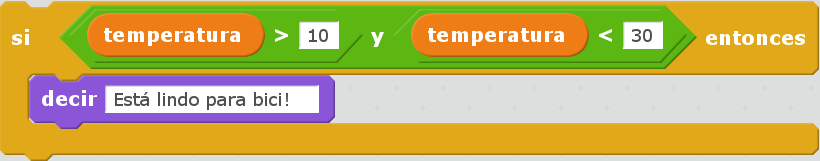
\includegraphics{files/img/u3/ej_sentencia_if.png}
\end{figure}

Una característica saliente para este tipo de comparaciones en Python es
la de asemejar al lenguaje natural, por lo que podemos implementar la
comparación previa haciendo:

\begin{Verbatim}[commandchars=\\\{\}]
\PYG{k}{if} \PYG{l+m+mi}{10} \PYG{o}{\PYGZlt{}} \PYG{n}{temperatura} \PYG{o}{\PYGZlt{}} \PYG{l+m+mi}{30}\PYG{p}{:}
    \PYG{k}{print}\PYG{p}{(}\PYG{l+s}{\PYGZsq{}}\PYG{l+s}{Está lindo para bici!}\PYG{l+s}{\PYGZsq{}}\PYG{p}{)}
\end{Verbatim}

\textbf{¿Qué acciones se ejecutan al cumplirse la condición?}

Una cuestión muy importante es indentar tal como se ha hecho en el
ejemplo, es decir, aseguraros de dejar una sangría en las líneas debajo
de los 2 puntos (:) que se deben ejecutar en caso que la condición de la
pregunta se cumpla.

Todo lenguaje de programación tiene en su sintaxis un modo de
identificar las acciones que forman parte de un bloque, en Python esto
es a partir de la sangría.


\subsection{Sentencia \emph{if..else}}
\label{Unidad03:sentencia-if-else}
Nuestro interés inicial era que el programa nos dijera si podemos ir en
auto o en bicicleta, y el ejemplo anterior solo nos dice algo cuando
podemos ir en bici, pero no dice o hace nada cuando la condición no se
cumple. Para estos casos existe un condicional llamado \textbf{*else*}(del inglés si no), que se usa conjuntamente con if y que sirve para
ejecutar ciertas instrucciones en caso de que la condición de la
sentencia if no se cumpla. Por ejemplo:

\begin{Verbatim}[commandchars=\\\{\}]
\PYG{k}{if} \PYG{p}{(}\PYG{n}{temperatura} \PYG{o}{\PYGZgt{}} \PYG{l+m+mi}{10}\PYG{p}{)} \PYG{o+ow}{and} \PYG{p}{(}\PYG{n}{temperatura} \PYG{o}{\PYGZlt{}} \PYG{l+m+mi}{30}\PYG{p}{)}\PYG{p}{:}
    \PYG{k}{print}\PYG{p}{(}\PYG{l+s}{\PYGZsq{}}\PYG{l+s}{Está lindo para ir en bici}\PYG{l+s}{\PYGZsq{}}\PYG{p}{)}
\PYG{k}{else}\PYG{p}{:}
    \PYG{k}{print}\PYG{p}{(}\PYG{l+s}{\PYGZsq{}}\PYG{l+s}{Te recomiendo ir en cole}\PYG{l+s}{\PYGZsq{}}\PYG{p}{)}
\end{Verbatim}

\begin{Verbatim}[commandchars=\\\{\}]
Está lindo para ir en bici
\end{Verbatim}

Esto se lee como \emph{si temperatura es mayor o igual a 10 y temperatura es
menor que 30, entonces mostrar el mensaje `Está lindo para ir en bici',
sino mostrar el mensaje `Te recomiendo ir en cole'}. Siempre se
ejecutará una opción u otra, dependiendo del valor de la variable
temperatura. Por lo que en este punto podemos decir que el código se
bifurca en dos caminos diferentes dependiendo de una condición (que en
este caso es el valor de la variable temperatura).
\begin{figure}[htbp]
\centering

\includegraphics{files/img/u3/ej_sentencia_if_else.png}
\end{figure}

En este caso también tenemos que prestar atención a la indentación
utilizada. La sentencia \emph{else} se escribe al mismo nivel que la
sentencia \emph{if}, y las sentencias que se deben ejecutar en caso de no se
cumpla la condición if, deben ir indentadas también.

Una versión más completa del programa podría ser la siguiente:

\begin{Verbatim}[commandchars=\\\{\}]
\PYG{n}{temperatura} \PYG{o}{=} \PYG{n+nb}{int}\PYG{p}{(}\PYG{n+nb}{input}\PYG{p}{(}\PYG{l+s}{\PYGZsq{}}\PYG{l+s}{Ingrese la temperatura en ºC:}\PYG{l+s}{\PYGZsq{}}\PYG{p}{)}\PYG{p}{)}

\PYG{k}{if} \PYG{p}{(}\PYG{n}{temperatura} \PYG{o}{\PYGZgt{}} \PYG{l+m+mi}{10}\PYG{p}{)} \PYG{o+ow}{and} \PYG{p}{(}\PYG{n}{temperatura} \PYG{o}{\PYGZlt{}} \PYG{l+m+mi}{30}\PYG{p}{)}\PYG{p}{:}
    \PYG{k}{print}\PYG{p}{(}\PYG{l+s}{\PYGZsq{}}\PYG{l+s}{Está lindo para ir en bici}\PYG{l+s}{\PYGZsq{}}\PYG{p}{)}
\PYG{k}{else}\PYG{p}{:}
    \PYG{k}{print}\PYG{p}{(}\PYG{l+s}{\PYGZsq{}}\PYG{l+s}{Te recomiendo ir en cole}\PYG{l+s}{\PYGZsq{}}\PYG{p}{)}

\PYG{k}{print}\PYG{p}{(}\PYG{l+s}{\PYGZsq{}}\PYG{l+s}{Que tenga buen día!}\PYG{l+s}{\PYGZsq{}}\PYG{p}{)}
\end{Verbatim}

\begin{Verbatim}[commandchars=\\\{\}]
Ingrese la temperatura en ºC:12
Deberías ser amable con el medio ambiente e ir en bicicleta
Que tenga buen día!
\end{Verbatim}

En este caso consultamos por la temperatura, pidiendole al usuario que
la ingrese por teclado (para esto utilizamos la función \emph{input} que
vimos en la Unidad 1). Luego mostramos en patalla lo que corresponda
según el valor ingresado, y por último mostramos el mensaje `Que tenga
buen día!'. Es importante mencionar que la última sentencia siempre se
ejecutará, la bifurcación se produce solamente entre las sentencias que
estan dentro del if y el else, lo restante se seguirá ejecutando de
manera secuencial.
\begin{figure}[htbp]
\centering

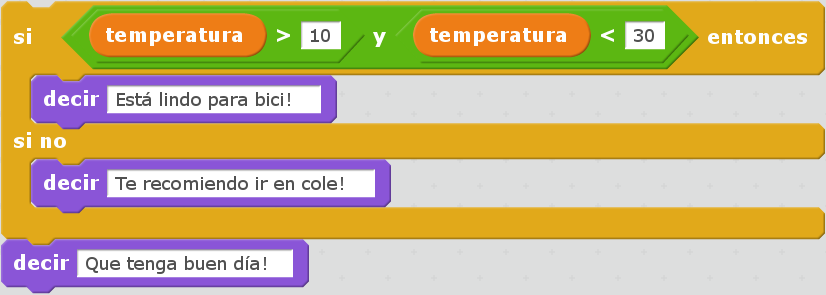
\includegraphics{files/img/u3/ej_sentencia_if_else_completa.png}
\end{figure}


\subsection{Estructura de selección múltiple \emph{if..elif..else}}
\label{Unidad03:estructura-de-seleccion-multiple-if-elif-else}
En los dos casos previos la secuencia de ejecución del programa tiene
solamente dos alternativas, si la condición es verdadera (\code{True}) o si
es falsa (\code{False}), incluso puede no existir un camino por la
alternativa falsa, tal como se planteó en el primer ejemplo.

Las estructuras de selección múltiple sirven para evaluar mas de una
condición y por ende posibilitar varios caminos de ejecución del
programa. En Python, la forma de esta estructura es del siguiente modo:

\begin{Verbatim}[commandchars=\\\{\}]
\PYG{k}{if} \PYG{n}{condicion1}\PYG{p}{:}
    \PYG{n}{acciones}
    \PYG{o}{.}\PYG{o}{.}\PYG{o}{.}
\PYG{k}{elif} \PYG{n}{condicion2}\PYG{p}{:}
    \PYG{n}{acciones}
    \PYG{o}{.}\PYG{o}{.}\PYG{o}{.}
\PYG{k}{elif} \PYG{n}{condicion3}\PYG{p}{:}
    \PYG{n}{acciones}
    \PYG{o}{.}\PYG{o}{.}\PYG{o}{.}
\PYG{k}{else}\PYG{p}{:}
    \PYG{n}{acciones}
    \PYG{o}{.}\PYG{o}{.}\PYG{o}{.}
\end{Verbatim}

La interpretación de esta sentencia significa que cuando cumpla alguna
de las condiciones ingresará al bloque de acciones correspondientes y,
en caso que no cumpla con ninguna, ejecutará las acciones del \code{else},
que podría ser omitido si no son necesarias acciones por defecto.

Veamos un ejemplo para mejorar la comprensión. Se lee una nota numérica
de una evaluación (0..100) y el programa debe mostrar una calificación
cualitativa según la siguiente escala:
\begin{itemize}
\item {} 
Insuficiente (nota \textless{} 60)

\item {} 
Aprobado (60 \textless{}= nota \textless{} 70)

\item {} 
Bueno (70 \textless{}= nota \textless{} 80)

\item {} 
Muy Bueno (80 \textless{}= nota \textless{} 90)

\item {} 
Distinguido (90 \textless{}= nota \textless{} 100)

\item {} 
Sobresaliente (nota = 100)

\end{itemize}

\begin{Verbatim}[commandchars=\\\{\}]
\PYG{c}{\PYGZsh{} Lectura de la nota}
\PYG{n}{nota} \PYG{o}{=} \PYG{n+nb}{int}\PYG{p}{(}\PYG{n+nb}{input}\PYG{p}{(}\PYG{l+s}{\PYGZsq{}}\PYG{l+s}{Ingrese la nota (0..100): }\PYG{l+s}{\PYGZsq{}}\PYG{p}{)}\PYG{p}{)}
\PYG{c}{\PYGZsh{} Decide la calif. correspondiente}
\PYG{k}{if} \PYG{n}{nota} \PYG{o}{\PYGZlt{}} \PYG{l+m+mi}{60}\PYG{p}{:}
    \PYG{n}{calif} \PYG{o}{=} \PYG{l+s}{\PYGZdq{}}\PYG{l+s}{Insuficiente}\PYG{l+s}{\PYGZdq{}}
\PYG{k}{elif} \PYG{l+m+mi}{60} \PYG{o}{\PYGZlt{}}\PYG{o}{=} \PYG{n}{nota} \PYG{o}{\PYGZlt{}} \PYG{l+m+mi}{70}\PYG{p}{:}
    \PYG{n}{calif} \PYG{o}{=} \PYG{l+s}{\PYGZdq{}}\PYG{l+s}{Aprobado}\PYG{l+s}{\PYGZdq{}}
\PYG{k}{elif} \PYG{l+m+mi}{70} \PYG{o}{\PYGZlt{}}\PYG{o}{=} \PYG{n}{nota} \PYG{o}{\PYGZlt{}} \PYG{l+m+mi}{80}\PYG{p}{:}
    \PYG{n}{calif} \PYG{o}{=} \PYG{l+s}{\PYGZdq{}}\PYG{l+s}{Bueno}\PYG{l+s}{\PYGZdq{}}
\PYG{k}{elif} \PYG{l+m+mi}{80} \PYG{o}{\PYGZlt{}}\PYG{o}{=} \PYG{n}{nota} \PYG{o}{\PYGZlt{}} \PYG{l+m+mi}{90}\PYG{p}{:}
    \PYG{n}{calif} \PYG{o}{=} \PYG{l+s}{\PYGZdq{}}\PYG{l+s}{Muy Bueno}\PYG{l+s}{\PYGZdq{}}
\PYG{k}{elif} \PYG{l+m+mi}{90} \PYG{o}{\PYGZlt{}}\PYG{o}{=} \PYG{n}{nota} \PYG{o}{\PYGZlt{}} \PYG{l+m+mi}{100}\PYG{p}{:}
    \PYG{n}{calif} \PYG{o}{=} \PYG{l+s}{\PYGZdq{}}\PYG{l+s}{Distinguido}\PYG{l+s}{\PYGZdq{}}
\PYG{k}{else}\PYG{p}{:}
    \PYG{n}{calif} \PYG{o}{=} \PYG{l+s}{\PYGZdq{}}\PYG{l+s}{Sobresaliente}\PYG{l+s}{\PYGZdq{}}
\PYG{c}{\PYGZsh{} Mensaje alusivo}
\PYG{k}{print}\PYG{p}{(}\PYG{l+s}{\PYGZdq{}}\PYG{l+s}{Calificación: }\PYG{l+s}{\PYGZdq{}}\PYG{p}{,} \PYG{n}{calif}\PYG{p}{)}
\end{Verbatim}

\begin{Verbatim}[commandchars=\\\{\}]
Ingrese la nota (0..100): 98
Calificación:  Distinguido
\end{Verbatim}

Como se observa, cada expresión condicional planteada es exluyente de
las demás, por lo que no puede cumplir con mas de una a la vez. Ahora,
podría existir un planteo donde se cumplan más de una condición y la
pregunta obvia es, ¿qué sucede en ese caso?

En el siguiente programa, ¿qué mensaje se muestra en pantalla?

\begin{Verbatim}[commandchars=\\\{\}]
\PYG{n}{val} \PYG{o}{=} \PYG{l+m+mi}{85}
\PYG{k}{if} \PYG{n}{val} \PYG{o}{\PYGZgt{}} \PYG{l+m+mi}{81}\PYG{p}{:}
    \PYG{k}{print}\PYG{p}{(}\PYG{l+s}{\PYGZdq{}}\PYG{l+s}{opción 1}\PYG{l+s}{\PYGZdq{}}\PYG{p}{)}
\PYG{k}{elif} \PYG{n}{val} \PYG{o}{\PYGZgt{}} \PYG{l+m+mi}{82}\PYG{p}{:}
    \PYG{k}{print}\PYG{p}{(}\PYG{l+s}{\PYGZdq{}}\PYG{l+s}{opción 2}\PYG{l+s}{\PYGZdq{}}\PYG{p}{)}
\PYG{k}{elif} \PYG{n}{val} \PYG{o}{\PYGZgt{}} \PYG{l+m+mi}{83}\PYG{p}{:}
    \PYG{k}{print}\PYG{p}{(}\PYG{l+s}{\PYGZdq{}}\PYG{l+s}{opción 3}\PYG{l+s}{\PYGZdq{}}\PYG{p}{)}
\end{Verbatim}


\subsection{Estructuras anidadas}
\label{Unidad03:estructuras-anidadas}
Retomando el ejemplo del programa anterior, supongamos ahora que también
queremos considerar la distancia que se debe recorrer. En este caso
deberíamos preguntar por la distancia, pero también por la temperatura.
Para que en los casos donde la temperatura sea agradable, la distancia
no sea demasiado larga como para ir en bicicleta.

Para estos casos, se pueden utilizar estructuras anidadas, es decir, en
el bloque de código que se ejecutará en caso de cumplirse o no una
determina condición, podemos poner una nueva estructura de control, por
ejemplo un nuevo \emph{if}.

Reescribamos el código anterior para que considere esta nueva condición,
y veamos como usar estructuras anidadas:

\begin{Verbatim}[commandchars=\\\{\}]
\PYG{n}{temperatura} \PYG{o}{=} \PYG{n+nb}{int}\PYG{p}{(}\PYG{n+nb}{input}\PYG{p}{(}\PYG{l+s}{\PYGZsq{}}\PYG{l+s}{Ingrese la temperatura en ºC:}\PYG{l+s}{\PYGZsq{}}\PYG{p}{)}\PYG{p}{)}
\PYG{n}{distancia} \PYG{o}{=} \PYG{n+nb}{int}\PYG{p}{(}\PYG{n+nb}{input}\PYG{p}{(}\PYG{l+s}{\PYGZsq{}}\PYG{l+s}{Ingrese la distancia a recorrer en km:}\PYG{l+s}{\PYGZsq{}}\PYG{p}{)}\PYG{p}{)}

\PYG{k}{if} \PYG{p}{(}\PYG{n}{temperatura} \PYG{o}{\PYGZgt{}} \PYG{l+m+mi}{10}\PYG{p}{)} \PYG{o+ow}{and} \PYG{p}{(}\PYG{n}{temperatura} \PYG{o}{\PYGZlt{}} \PYG{l+m+mi}{30}\PYG{p}{)}\PYG{p}{:}
    \PYG{k}{if} \PYG{p}{(}\PYG{n}{distancia} \PYG{o}{\PYGZlt{}}\PYG{o}{=} \PYG{l+m+mi}{15}\PYG{p}{)}\PYG{p}{:}
        \PYG{k}{print}\PYG{p}{(}\PYG{l+s}{\PYGZsq{}}\PYG{l+s}{Está lindo para ir en bici}\PYG{l+s}{\PYGZsq{}}\PYG{p}{)}
    \PYG{k}{else}\PYG{p}{:}
        \PYG{k}{print}\PYG{p}{(}\PYG{l+s}{\PYGZsq{}}\PYG{l+s}{Está lindo, pero es lejos, le recomiendo ir en auto}\PYG{l+s}{\PYGZsq{}}\PYG{p}{)}
\PYG{k}{else}\PYG{p}{:}
    \PYG{k}{print}\PYG{p}{(}\PYG{l+s}{\PYGZsq{}}\PYG{l+s}{La temperatura no es agradable, le recomiendo ir en auto.}\PYG{l+s}{\PYGZsq{}}\PYG{p}{)}

\PYG{k}{print}\PYG{p}{(}\PYG{l+s}{\PYGZsq{}}\PYG{l+s}{Que tenga buen día!}\PYG{l+s}{\PYGZsq{}}\PYG{p}{)}
\end{Verbatim}

\begin{Verbatim}[commandchars=\\\{\}]
Ingrese la temperatura en ºC:15
Ingrese la distancia a recorrer en km:1
Está lindo para ir en bici
Que tenga buen día!
\end{Verbatim}

En este caso si se cumple la condición de que la variable temperatura
contiene un valor entre 10 y 29, se pasa a considerar el valor de la
variable distancia; si esta es menor o igual a 15, se muestra el mensaje
\emph{`Está lindo para ir en bici'}, en caso contrario, se muestra el mensaje
\emph{`Está lindo, pero es lejos, le recomiendo ir en auto'}. Por otro lado,
si el valor de la variable temperatura no esta entre 10 y 29, se seguirá
mostrando el mensaje \emph{`La temperatura no es agradable, le recomiendo ir
en auto'}. Lo mismo sucede con la última sentencia, la cual mostrará el
mensaje \emph{`Que tenga buen día!'} independientemente del valor de las
variables \emph{temperatura} y \emph{distancia}


\section{Estructuras repetitivas}
\label{Unidad03:estructuras-repetitivas}
Ahora podemos dotar a nuestros programas de mayor complejidad,
combinando y anidando las estructuras condicionales vistas. Sin embargo,
aún tenemos una limitante, cada instrucción tendrá vida al momento de
ser ejecutada e inmediamente después no se ejecutará más hasta que se el
programa se invoque nuevamente.

Imaginemos que debemos consultar la pregunta de la temperatura a cientos
de miles de personas, deberíamos ejecutar cientos de miles de veces el
programa, iniciandolo y esperando su finalización para repetir el
proceso una y otra vez. Se hace evidente la ausencia de una estructura
que permita repetir cuantas veces se requiera una determinada acción,
aquí es donde entran en acción las estructuras repetitivas.


\subsection{Sentencia \emph{while}}
\label{Unidad03:sentencia-while}
El \emph{while} permite repetir una serie de acciones mientras que una
determinada expresión (o condición) se cumpla, en caso contrario, se
finaliza la repetición.

Una expresión se cumple cuando arroja un resultado verdadero, que en
Python es \code{True}. La estructura del \emph{while} es la siguiente:

\begin{Verbatim}[commandchars=\\\{\}]
while \PYGZlt{}expresion\PYGZgt{}
    accion1
    accion2
    ...
    accionN
\end{Verbatim}

Tal como se explicó previamente, las acciones que se repiten en cada
iteración son aquellas que tienen sangría, lo que indica que son partes
del ciclo \emph{while}.


\subsubsection{Bucles condicionales}
\label{Unidad03:bucles-condicionales}
Veamos un ejemplo donde se le pregunte el valor de temperatura a 5
personas y sugiera ir caminando si el clima es agradable (mayor a 16°C)
o en caso contrario en vehículo. Tomemos una estrategia para resolver el
problema:
\begin{enumerate}
\item {} 
Leemos una temperatura que se ingresa por teclado

\item {} 
Escribimos en pantalla un mensaje según la temperatura

\item {} 
Repetir los dos pasos previos un total de cinco veces

\end{enumerate}

\textbf{Pasos 1 y 2}

\begin{Verbatim}[commandchars=\\\{\}]
\PYG{n}{temperatura} \PYG{o}{=} \PYG{n+nb}{int}\PYG{p}{(}\PYG{n+nb}{input}\PYG{p}{(}\PYG{l+s}{\PYGZsq{}}\PYG{l+s}{Ingrese la temperatura en ºC:}\PYG{l+s}{\PYGZsq{}}\PYG{p}{)}\PYG{p}{)}
\PYG{k}{if} \PYG{p}{(}\PYG{n}{temperatura} \PYG{o}{\PYGZgt{}} \PYG{l+m+mi}{16}\PYG{p}{)}\PYG{p}{:}
    \PYG{k}{print}\PYG{p}{(}\PYG{l+s}{\PYGZsq{}}\PYG{l+s}{Vas caminando}\PYG{l+s}{\PYGZsq{}}\PYG{p}{)}
\PYG{k}{else}\PYG{p}{:}
    \PYG{k}{print}\PYG{p}{(}\PYG{l+s}{\PYGZsq{}}\PYG{l+s}{Mucho frío, en vehículo}\PYG{l+s}{\PYGZsq{}}\PYG{p}{)}
\end{Verbatim}

\textbf{Paso 3}

Debemos englobar los pasos previos en una estructura que repita 5 veces.
Pensemos lo anterior como un único bloque denominado \emph{Pasos1y2}, y una
manera de controlar cinco repeticiones. Para ésto, usamos una variable
con un valor inicial conocido (1) que incrementamos en una unidad luego
de cada ejecución del bloque que denominamos \emph{Pasos1y2}. La estructura
de nuestro programa podría ser la siguiente:

\begin{Verbatim}[commandchars=\\\{\}]
\PYG{n}{vez} \PYG{o}{=} \PYG{l+m+mi}{1}
\PYG{k}{while} \PYG{n}{vez} \PYG{o}{\PYGZlt{}}\PYG{o}{=} \PYG{l+m+mi}{5}\PYG{p}{:}
    \PYG{n}{Pasos1y2}
    \PYG{n}{vez} \PYG{o}{=} \PYG{n}{vez} \PYG{o}{+} \PYG{l+m+mi}{1}
\end{Verbatim}

Ahora bien, cuando finaliza la ejecución de la instrucción
\code{vez = vez + 1} la estructura iterativa evalúa nuevamente la expresión
\code{vez \textless{}= 5} cuyo resultado puede ser cierto o no (\code{True} o
\code{False}). Si el resultado es \code{True}, entonces el ciclo continuará
con las acciones contenidas, re-evaluando la expresión en cada
itereación y finalizando cuando sea \code{False}, es decir, cuando la
variable \code{vez} ya no sea menor o igual que 5.

Ahora que ya hemos desmenuzado el inofensivo código previo, podemos
pasar a la versión final del pequeño programa.

\begin{Verbatim}[commandchars=\\\{\}]
\PYG{n}{vez} \PYG{o}{=} \PYG{l+m+mi}{1}
\PYG{k}{while} \PYG{n}{vez} \PYG{o}{\PYGZlt{}}\PYG{o}{=} \PYG{l+m+mi}{5}\PYG{p}{:}
    \PYG{n}{temperatura} \PYG{o}{=} \PYG{n+nb}{int}\PYG{p}{(}\PYG{n+nb}{input}\PYG{p}{(}\PYG{l+s}{\PYGZsq{}}\PYG{l+s}{Ingrese la temperatura en ºC:}\PYG{l+s}{\PYGZsq{}}\PYG{p}{)}\PYG{p}{)}
    \PYG{k}{if} \PYG{p}{(}\PYG{n}{temperatura} \PYG{o}{\PYGZgt{}} \PYG{l+m+mi}{16}\PYG{p}{)}\PYG{p}{:}
        \PYG{k}{print}\PYG{p}{(}\PYG{l+s}{\PYGZsq{}}\PYG{l+s}{Vas caminando}\PYG{l+s}{\PYGZsq{}}\PYG{p}{)}
    \PYG{k}{else}\PYG{p}{:}
        \PYG{k}{print}\PYG{p}{(}\PYG{l+s}{\PYGZsq{}}\PYG{l+s}{Mucho frío, en vehículo}\PYG{l+s}{\PYGZsq{}}\PYG{p}{)}
    \PYG{n}{vez} \PYG{o}{=} \PYG{n}{vez} \PYG{o}{+} \PYG{l+m+mi}{1}
\end{Verbatim}

\begin{Verbatim}[commandchars=\\\{\}]
Ingrese la temperatura en ºC:12
Mucho frío, en vehículo
Ingrese la temperatura en ºC:16
Mucho frío, en vehículo
Ingrese la temperatura en ºC:17
Vas caminando
Ingrese la temperatura en ºC:18
Vas caminando
Ingrese la temperatura en ºC:20
Vas caminando
\end{Verbatim}

Este tipo de bucle, donde la cantidad de iteraciones depende de una
condición es denominado como \textbf{bucles o lazos condicionales} y cuenta
con dos características destacables:
\begin{itemize}
\item {} 
El valor a ser evaluado en la expresión debe estar definido

\item {} 
En cada iteración el valor a ser evaluado en la expresión debe
modificarse

\end{itemize}

El primer item evita obtener un mensaje de error, ya que no es posible
evaluar una expresión con un valor que aún no ha sido definido, es
decir, que no tiene asignado algún valor válido.

La segunda característica evita tener un \textbf{bucle infinito} y por ende
un programa que nunca finalice. Este tipo de errores es más difícil de
detectar, ya que a priori el ejemplo parecería correcto.


\subsubsection{Bucles interactivos}
\label{Unidad03:bucles-interactivos}
Otro tipo bucle para el que la estructura \emph{while} se adapta fácilmente
es aquellos donde la repetición depende de un valor que ingresa el
usuario, es decir, para aquellos programas donde la condición de corte o
repetición sea interactiva. Veamos un ejemplo en el que se calcula el
promedio a partir del ingreso por parte del usuario de valores numéricos
enteros.

Pensemos una posible estrategia para su solución: el programa le
solicitará ingresar un nuevo valor numérico mientras que el usuario
ingrese \emph{si}, a su vez deberá ir sumando estos valores y contándolos.
Veamos el pseudocódigo del algoritmo mencionado:

\begin{Verbatim}[commandchars=\\\{\}]
Inicializar variable suma para sumar los números
Inicializar variable cant para contar los números
Inicializar variable mas\PYGZus{}datos donde se almacenará la respuesta del usuario (si/no)
Mientras la variable mas\PYGZus{}datos sea si:
    Leer en x el nuevo valor numérico
    Sumarlo a la variable suma
    Contarlo
    Pregutar al usuario si sigue ingresando números
Mostrar en pantalla el promedio
\end{Verbatim}

Ahora veamos lo directa que es la traducción del algoritmo al lenguaje
Python:

\begin{Verbatim}[commandchars=\\\{\}]
\PYG{n}{suma} \PYG{o}{=} \PYG{l+m+mf}{0.0}
\PYG{n}{cant} \PYG{o}{=} \PYG{l+m+mi}{0}
\PYG{n}{mas\PYGZus{}datos} \PYG{o}{=} \PYG{l+s}{\PYGZsq{}}\PYG{l+s}{si}\PYG{l+s}{\PYGZsq{}}
\PYG{k}{while} \PYG{n}{mas\PYGZus{}datos} \PYG{o}{==} \PYG{l+s}{\PYGZsq{}}\PYG{l+s}{si}\PYG{l+s}{\PYGZsq{}}\PYG{p}{:}
    \PYG{n}{x} \PYG{o}{=} \PYG{n+nb}{int}\PYG{p}{(}\PYG{n+nb}{input}\PYG{p}{(}\PYG{l+s}{\PYGZsq{}}\PYG{l+s}{Ingrese valor}\PYG{l+s}{\PYGZsq{}}\PYG{p}{)}\PYG{p}{)}
    \PYG{n}{suma} \PYG{o}{=} \PYG{n}{suma} \PYG{o}{+} \PYG{n}{x}
    \PYG{n}{cant} \PYG{o}{=} \PYG{n}{cant} \PYG{o}{+} \PYG{l+m+mi}{1}
    \PYG{n}{mas\PYGZus{}datos} \PYG{o}{=} \PYG{n+nb}{input}\PYG{p}{(}\PYG{l+s}{\PYGZsq{}}\PYG{l+s}{¿Mas valores (si/no)?}\PYG{l+s}{\PYGZsq{}}\PYG{p}{)}
\PYG{k}{print}\PYG{p}{(}\PYG{l+s}{\PYGZsq{}}\PYG{l+s}{El promedio de valores es}\PYG{l+s}{\PYGZsq{}}\PYG{p}{,} \PYG{n}{suma}\PYG{o}{/}\PYG{n}{cant}\PYG{p}{)}
\end{Verbatim}

\begin{Verbatim}[commandchars=\\\{\}]
Ingrese valor12
¿Mas valores (si/no)?si
Ingrese valor3
¿Mas valores (si/no)?si
Ingrese valor44
¿Mas valores (si/no)?no
El promedio de valores es 19.666666666666668
\end{Verbatim}

La limitación que encontramos está dada por la incomodidad de tener que
ingresar dos valores por ciclo, uno para el dato numérico y otro para
controlar si el usuario desea continuar o no. En ciertos casos puede ser
la única alternativa, sin embargo, en otros se puede utilizar los bucles
centinelas que se describen a continuación.


\subsubsection{Bucles centinelas}
\label{Unidad03:bucles-centinelas}
Otro tipo de bucles denominados centinelas, son aquellos donde la
condición de corte tiene que ver con un valor que se diferencia del
patrón que se ingresará y, será útil para discernir el momento en que
corresponda continuar o bien finalizar la repetición.

Para el caso del cálculo del promedio, suponiendo que todos los valores
serán siempre positivos podríamos tomar la estrategia de controlar que
el valor ingresado sea mayor a cero para continuar la iteración. El
pseudocódigo, sin detalles, sería similar al siguiente:

\begin{Verbatim}[commandchars=\\\{\}]
Leer en x el primer valor numérico
Mientras el valor x no sea el centinela:
    Sumarlo a la variable suma
    Contarlo
    Leer en x el nuevo valor numérico
Mostrar en pantalla el promedio
\end{Verbatim}

Veamos la implementación del amigable programa en Python:

\begin{Verbatim}[commandchars=\\\{\}]
\PYG{n}{suma} \PYG{o}{=} \PYG{l+m+mf}{0.0}
\PYG{n}{cant} \PYG{o}{=} \PYG{l+m+mi}{0}
\PYG{n}{x} \PYG{o}{=} \PYG{n+nb}{int}\PYG{p}{(}\PYG{n+nb}{input}\PYG{p}{(}\PYG{l+s}{\PYGZsq{}}\PYG{l+s}{Ingrese valor (negativo para salir)}\PYG{l+s}{\PYGZsq{}}\PYG{p}{)}\PYG{p}{)}
\PYG{k}{while} \PYG{n}{x} \PYG{o}{\PYGZgt{}} \PYG{l+m+mi}{0}\PYG{p}{:}
    \PYG{n}{suma} \PYG{o}{=} \PYG{n}{suma} \PYG{o}{+} \PYG{n}{x}
    \PYG{n}{cant} \PYG{o}{=} \PYG{n}{cant} \PYG{o}{+} \PYG{l+m+mi}{1}
    \PYG{n}{x} \PYG{o}{=} \PYG{n+nb}{int}\PYG{p}{(}\PYG{n+nb}{input}\PYG{p}{(}\PYG{l+s}{\PYGZsq{}}\PYG{l+s}{Ingrese valor (negativo para salir)}\PYG{l+s}{\PYGZsq{}}\PYG{p}{)}\PYG{p}{)}
\PYG{k}{print}\PYG{p}{(}\PYG{l+s}{\PYGZsq{}}\PYG{l+s}{El promedio de valores es}\PYG{l+s}{\PYGZsq{}}\PYG{p}{,} \PYG{n}{suma}\PYG{o}{/}\PYG{n}{cant}\PYG{p}{)}
\end{Verbatim}

Se debe ser cuidadoso en mantener exactamente el mismo mensaje previo a
ingresar al ciclo y en la última instrucción para dar al usuario una
idea de continuidad viendo una y otra vez el mismo comportamiento.

Para el ejemplo expuesto, la limitación esta dada para aquellos casos
donde se ingresen valores negativos para ser incluídos en el cálculo del
promedio. Sin embargo, Python provee herramientas que permiten salvar
este inconveniente.

El problema consiste en:
\begin{enumerate}
\item {} 
Solicitar al usuario ingrese el valor numérico o que presione \emph{enter}
para salir

\item {} 
Evaluar en la expresión de corte para iterar mientras que el valor
ingresado no sea vacío

\item {} 
Realizar los cálculos

\end{enumerate}

\begin{Verbatim}[commandchars=\\\{\}]
\PYG{n}{suma} \PYG{o}{=} \PYG{l+m+mf}{0.0}
\PYG{n}{cant} \PYG{o}{=} \PYG{l+m+mi}{0}
\PYG{n}{x} \PYG{o}{=} \PYG{n+nb}{input}\PYG{p}{(}\PYG{l+s}{\PYGZsq{}}\PYG{l+s}{Ingrese valor (\PYGZlt{}enter\PYGZgt{} para salir)}\PYG{l+s}{\PYGZsq{}}\PYG{p}{)}
\PYG{k}{while} \PYG{n}{x} \PYG{o}{!=} \PYG{l+s}{\PYGZsq{}}\PYG{l+s}{\PYGZsq{}}\PYG{p}{:}
    \PYG{n}{suma} \PYG{o}{=} \PYG{n}{suma} \PYG{o}{+} \PYG{n+nb}{eval}\PYG{p}{(}\PYG{n}{x}\PYG{p}{)}
    \PYG{n}{cant} \PYG{o}{=} \PYG{n}{cant} \PYG{o}{+} \PYG{l+m+mi}{1}
    \PYG{n}{x} \PYG{o}{=} \PYG{n+nb}{input}\PYG{p}{(}\PYG{l+s}{\PYGZsq{}}\PYG{l+s}{Ingrese valor (\PYGZlt{}enter\PYGZgt{} para salir)}\PYG{l+s}{\PYGZsq{}}\PYG{p}{)}
\PYG{k}{print}\PYG{p}{(}\PYG{l+s}{\PYGZsq{}}\PYG{l+s}{El promedio de valores es}\PYG{l+s}{\PYGZsq{}}\PYG{p}{,} \PYG{n}{suma}\PYG{o}{/}\PYG{n}{cant}\PYG{p}{)}
\end{Verbatim}

\begin{Verbatim}[commandchars=\\\{\}]
Ingrese valor (\PYGZlt{}enter\PYGZgt{} para salir)12
Ingrese valor (\PYGZlt{}enter\PYGZgt{} para salir)\PYGZhy{}2
Ingrese valor (\PYGZlt{}enter\PYGZgt{} para salir)\PYGZhy{}3
Ingrese valor (\PYGZlt{}enter\PYGZgt{} para salir)23
Ingrese valor (\PYGZlt{}enter\PYGZgt{} para salir)2
Ingrese valor (\PYGZlt{}enter\PYGZgt{} para salir)
El promedio de valores es 6.4
\end{Verbatim}

El valor leído en \emph{x} no se convierte en un número entero, sino que se
lo mantiene como \emph{str} hasta el momento de sumarlo a la variable \emph{suma}
utilizando la función \emph{eval()}. Cuando el usuario presione enter el
caracter en \emph{x} será igual al caracter vacío y no ingresará al ciclo
\emph{while}.


\subsection{Sentencia \emph{for}}
\label{Unidad03:sentencia-for}
La sentencia \emph{for} provee otro modo de realizar bucles repetitivos en
Python. Si bien la elección de un bucle u otro muchas veces dependerá
del gusto o preferencia del programador, para ciertos casos suele ser
más cómoda una estructura que otra.

Veamos la sintaxis básica del bucle for:

\begin{Verbatim}[commandchars=\\\{\}]
for \PYGZlt{}var\PYGZgt{} in \PYGZlt{}secuencia\PYGZgt{}:
    accion1
    accion2
    ...
    accionN
\end{Verbatim}

El \emph{for} ejecuta el bloque de acciones tantas veces como elementos
contenga la \emph{secuencia}, y en cada iteración la variable \emph{var}
almacenará uno a uno sus valores.

El significado de secuencia para Python puede variar desde cadenas de
caracteres a listas de valores de tipos de datos ya vistos, simplifando
la definición, podemos definir una secuencia como todo tipo o estructura
de datos formada por elementos por los que se puede iterar.

Veamos un ejemplo, donde mostramos los caracteres de una cadena.

\begin{Verbatim}[commandchars=\\\{\}]
\PYG{n}{palabra} \PYG{o}{=} \PYG{l+s}{\PYGZsq{}}\PYG{l+s}{estimados}\PYG{l+s}{\PYGZsq{}}
\PYG{k}{for} \PYG{n}{letra} \PYG{o+ow}{in} \PYG{n}{palabra}\PYG{p}{:}
    \PYG{k}{print}\PYG{p}{(}\PYG{n}{letra}\PYG{p}{)}
\end{Verbatim}

\begin{Verbatim}[commandchars=\\\{\}]
\PYG{n}{e}
\PYG{n}{s}
\PYG{n}{t}
\PYG{n}{i}
\PYG{n}{m}
\PYG{n}{a}
\PYG{n}{d}
\PYG{n}{o}
\PYG{n}{s}
\end{Verbatim}

Al analizar el ejemplo vemos que la variable \emph{palabra} que contiene una
\textbf{cadena de caracteres, funciona como una secuencia}, y la variable
\emph{letra} en cada iteración toma automáticamente el caracter subsiguiente.


\subsection{Iteraciones sobre secuencias numéricas}
\label{Unidad03:iteraciones-sobre-secuencias-numericas}
Para iterar sobre secuencias numéricas combinamos el uso del \code{for} con
la función \code{range()}. Veamos un ejemplo de una iteración sobre 3
valores:

\begin{Verbatim}[commandchars=\\\{\}]
\PYG{k}{for} \PYG{n}{num} \PYG{o+ow}{in} \PYG{n+nb}{range}\PYG{p}{(}\PYG{l+m+mi}{3}\PYG{p}{)}\PYG{p}{:}
    \PYG{k}{print}\PYG{p}{(}\PYG{n}{num}\PYG{p}{)}
\end{Verbatim}

\begin{Verbatim}[commandchars=\\\{\}]
\PYG{l+m+mi}{0}
\PYG{l+m+mi}{1}
\PYG{l+m+mi}{2}
\end{Verbatim}

Cuando utilizamos la función \code{range()} con un único argumento como
dato, para el ejemplo previo el número 3, nos genera una secuencia de 3
valores, comenzando desde 0 y avanzando de a un valor, es decir, con
paso 1. Sin embargo, podemos cambiar este comportamiento indicando el
valor inicial y final haciendo \code{range(inicio,fin)}, por ejemplo, se se
desea iterar por valores numéricos entre 10 y 14:

\begin{Verbatim}[commandchars=\\\{\}]
\PYG{k}{for} \PYG{n}{num} \PYG{o+ow}{in} \PYG{n+nb}{range}\PYG{p}{(}\PYG{l+m+mi}{10}\PYG{p}{,}\PYG{l+m+mi}{14}\PYG{p}{)}\PYG{p}{:}
    \PYG{k}{print}\PYG{p}{(}\PYG{n}{num}\PYG{p}{)}
\end{Verbatim}

\begin{Verbatim}[commandchars=\\\{\}]
\PYG{l+m+mi}{10}
\PYG{l+m+mi}{11}
\PYG{l+m+mi}{12}
\PYG{l+m+mi}{13}
\end{Verbatim}

Se debe notar que el valor final no es alcanzado en la iteración.
También es posible indicarle el paso del incremento, como se deduce del
ejemplo previo, al indicar solamente el valor inicial y final, se da por
sentado que el incremento es de 1, cambiemos este comportamiento
utilizando \code{range(inicio, fin, paso)}:

\begin{Verbatim}[commandchars=\\\{\}]
\PYG{k}{for} \PYG{n}{num} \PYG{o+ow}{in} \PYG{n+nb}{range}\PYG{p}{(}\PYG{l+m+mi}{10}\PYG{p}{,}\PYG{l+m+mi}{19}\PYG{p}{,}\PYG{l+m+mi}{2}\PYG{p}{)}\PYG{p}{:}
    \PYG{k}{print}\PYG{p}{(}\PYG{n}{num}\PYG{p}{)}
\end{Verbatim}

\begin{Verbatim}[commandchars=\\\{\}]
\PYG{l+m+mi}{10}
\PYG{l+m+mi}{12}
\PYG{l+m+mi}{14}
\PYG{l+m+mi}{16}
\PYG{l+m+mi}{18}
\end{Verbatim}

Otra posibilidad es recorrer una secuencia numérica en sentido sentido
inverso, utilizando un incremento negativo y los valores de inicio y fin
consistentes:

\begin{Verbatim}[commandchars=\\\{\}]
\PYG{k}{for} \PYG{n}{num} \PYG{o+ow}{in} \PYG{n+nb}{range}\PYG{p}{(}\PYG{l+m+mi}{19}\PYG{p}{,}\PYG{l+m+mi}{10}\PYG{p}{,}\PYG{o}{\PYGZhy{}}\PYG{l+m+mi}{2}\PYG{p}{)}\PYG{p}{:}
    \PYG{k}{print}\PYG{p}{(}\PYG{n}{num}\PYG{p}{)}
\end{Verbatim}

\begin{Verbatim}[commandchars=\\\{\}]
\PYG{l+m+mi}{19}
\PYG{l+m+mi}{17}
\PYG{l+m+mi}{15}
\PYG{l+m+mi}{13}
\PYG{l+m+mi}{11}
\end{Verbatim}

Del resultado previo queda en evidencia que se mantiene la coherencia
respecto a excluir el último valor de la secuencia y a incluir el
inicial.

Veamos un ejemplo que resolvimos anteriormente utilizando el \code{while},
ahora usando \code{for}:

\begin{Verbatim}[commandchars=\\\{\}]
for vez in range(5)
    temperatura = int(input(\PYGZsq{}Ingrese la temperatura en ºC:\PYGZsq{}))
    if (temperatura \PYGZgt{} 16):
        print(\PYGZsq{}Vas caminando\PYGZsq{})
    else:
        print(\PYGZsq{}Mucho frío, en vehículo\PYGZsq{})
\end{Verbatim}

Como vemos, nos despreocupamos de la inicialización de la variable \emph{vez}
y de controlar su incremento, ya que esto se realiza automáticamente,
por lo que para ciclos que conocemos de antemano la cantidad de
iteraciones suele ser más simple y directo que el \code{while}.

La sentencia \code{for} en combinación con \code{range()} es una instrucción
muy potente y flexible, más aún al ser combinadas con otro tipo de
estructuras de datos como cadenas de caracteres y listas, que veremos en
secciones posteriores.


\section{Estructura de datos}
\label{Unidad03:estructura-de-datos}

\subsection{Listas}
\label{Unidad03:listas}
Hasta aquí todo dato procesado, manipulado y operado ha sido almacenado
en variables, sin embargo, para ciertos problemas no son suficientes.
Supongamos un caso donde leemos una serie de temperaturas mensuales
durante los últimos 10 años y que posteriormente queremos saber las
temperaturas que han superado la media.

Si utilizamos variables, deberíamos leer los 120 valores para calcular
el promedio y reingresar nuevamente las temperaturas mensuales para
corroborar aquellas que superaron la media. Claramente el usuario de
este programa no estará muy feliz de tener que tipear nuevamente la
totalidad de los datos.

Para este tipo de problemas y muchos otros más existe una estructuras
más compleja y de gran utilidad denominada \textbf{lista}.

A diferencia de una variable que contiene un dato por vez, una lista
puede almacenar varios en forma simultánea en diferentes posiciones, por
lo que para referirnos a uno de ellos necesitamos especificarle el
índice. Por ejemplo, en la siguiente lista denominada \emph{tempC} hay
almacenados tres valores numéricos flotantes, el primero está en la
posición 0, el segundo en la posición 1 y, el tercero en la posición 2:

\begin{tabulary}{\linewidth}{|L|L|L|}
\hline
\textsf{\relax 
12.2
} & \textsf{\relax 
33.3
} & \textsf{\relax 
12.1
}\\
\hline
0
 & 
1
 & 
2
\\
\hline\end{tabulary}


Para \textbf{declarar e inicializar} una lista vacía y otra con esos tres
valores haremos:

\begin{Verbatim}[commandchars=\\\{\}]
\PYG{c}{\PYGZsh{} Lista vacia}
\PYG{n}{vacia} \PYG{o}{=} \PYG{p}{[}\PYG{p}{]}
\PYG{c}{\PYGZsh{} Lista con 3 valores flotantes}
\PYG{n}{tempC} \PYG{o}{=} \PYG{p}{[}\PYG{l+m+mf}{12.2}\PYG{p}{,} \PYG{l+m+mf}{33.3}\PYG{p}{,} \PYG{l+m+mf}{12.1}\PYG{p}{]}
\end{Verbatim}

Para acceder a un elemento específico, debemos utilizar el identificador
de la lista, seguido del índice entre corchetes (cualquier expresión
entera), veamos un ejemplo donde realizamos las siguientes acciones:
\begin{enumerate}
\item {} 
Imprimir en pantalla el segundo valor (la posición 1 porque empezamos
a contar desde 0)

\item {} 
Asignarle un nuevo valor que lo reemplace y volver a imprimirlo

\item {} 
Mostrar todo el contenido de la lista usando un bucle \emph{for}

\item {} 
Mostrar aquellas temperaturas que superaron el promedio

\end{enumerate}

\begin{Verbatim}[commandchars=\\\{\}]
\PYG{c}{\PYGZsh{} Elemento 1 de la lista}
\PYG{k}{print}\PYG{p}{(}\PYG{l+s}{\PYGZdq{}}\PYG{l+s}{2do elemento:}\PYG{l+s}{\PYGZdq{}}\PYG{p}{,} \PYG{n}{tempC}\PYG{p}{[}\PYG{l+m+mi}{1}\PYG{p}{]}\PYG{p}{)}

\PYG{c}{\PYGZsh{} Reemplaza el elemento 1 con 100}
\PYG{n}{tempC}\PYG{p}{[}\PYG{l+m+mi}{1}\PYG{p}{]} \PYG{o}{=} \PYG{l+m+mi}{100}
\PYG{k}{print}\PYG{p}{(}\PYG{l+s}{\PYGZdq{}}\PYG{l+s}{2do elemento modificado:}\PYG{l+s}{\PYGZdq{}}\PYG{p}{,}\PYG{n}{tempC}\PYG{p}{[}\PYG{l+m+mi}{1}\PYG{p}{]}\PYG{p}{)}

\PYG{c}{\PYGZsh{} Lista completa y calculo de promedio}
\PYG{k}{print}\PYG{p}{(}\PYG{l+s}{\PYGZdq{}}\PYG{l+s}{Lista:}\PYG{l+s}{\PYGZdq{}}\PYG{p}{)}
\PYG{n}{media} \PYG{o}{=} \PYG{l+m+mf}{0.0}
\PYG{k}{for} \PYG{n}{i} \PYG{o+ow}{in} \PYG{n}{tempC}\PYG{p}{:}
    \PYG{k}{print}\PYG{p}{(}\PYG{n}{i}\PYG{p}{)}
    \PYG{n}{media} \PYG{o}{=} \PYG{n}{media} \PYG{o}{+} \PYG{n}{i}
\PYG{n}{media} \PYG{o}{=} \PYG{n}{media}\PYG{o}{/}\PYG{l+m+mi}{3}

\PYG{c}{\PYGZsh{} Elementos que superan el promedio}
\PYG{k}{for} \PYG{n}{i} \PYG{o+ow}{in} \PYG{n}{tempC}\PYG{p}{:}
    \PYG{k}{if} \PYG{n}{i} \PYG{o}{\PYGZgt{}} \PYG{n}{media}\PYG{p}{:}
        \PYG{k}{print}\PYG{p}{(}\PYG{l+s}{\PYGZdq{}}\PYG{l+s}{La temperatura}\PYG{l+s}{\PYGZdq{}}\PYG{p}{,} \PYG{n}{i}\PYG{p}{,} \PYG{l+s}{\PYGZdq{}}\PYG{l+s}{superó la media}\PYG{l+s}{\PYGZdq{}}\PYG{p}{)}
\end{Verbatim}

\begin{Verbatim}[commandchars=\\\{\}]
2do elemento: 100
2do elemento modificado: 100
Lista:
12.2
100
12.1
La temperatura 100 superó la media
\end{Verbatim}

Como se observa en el ciclo iterativo previo, las listas son
perfectamente iterables en el \code{for}, ya que al igual que una cadena de
caracteres, es una secuencia de valores, la diferencia radica que en una
cadena los valores son caracteres mientras que en una lista pueden ser
de cualquier tipo y son llamados elementos o items.

Otro detalle es que una lista puede contener elementos de diferente
tipo, incluso otra lista. Veamos una lista que combine elementos de
distintos tipos:

\begin{Verbatim}[commandchars=\\\{\}]
\PYG{c}{\PYGZsh{} Lista que almacena distintos tipos de datos}
\PYG{n}{popurri} \PYG{o}{=} \PYG{p}{[}\PYG{l+m+mi}{12}\PYG{p}{,} \PYG{l+m+mf}{3.1415}\PYG{p}{,} \PYG{l+s}{\PYGZdq{}}\PYG{l+s}{amapola del 66}\PYG{l+s}{\PYGZdq{}}\PYG{p}{,} \PYG{n+nb+bp}{True}\PYG{p}{,} \PYG{n}{tempC}\PYG{p}{]}

\PYG{c}{\PYGZsh{} Imprimen los elementos}
\PYG{k}{print}\PYG{p}{(}\PYG{l+s}{\PYGZdq{}}\PYG{l+s}{1er elemento: }\PYG{l+s}{\PYGZdq{}}\PYG{p}{,} \PYG{n}{popurri}\PYG{p}{[}\PYG{l+m+mi}{0}\PYG{p}{]}\PYG{p}{)}
\PYG{k}{print}\PYG{p}{(}\PYG{l+s}{\PYGZdq{}}\PYG{l+s}{2do elemento: }\PYG{l+s}{\PYGZdq{}}\PYG{p}{,} \PYG{n}{popurri}\PYG{p}{[}\PYG{l+m+mi}{1}\PYG{p}{]}\PYG{p}{)}
\PYG{k}{print}\PYG{p}{(}\PYG{l+s}{\PYGZdq{}}\PYG{l+s}{3er elemento: }\PYG{l+s}{\PYGZdq{}}\PYG{p}{,} \PYG{n}{popurri}\PYG{p}{[}\PYG{l+m+mi}{2}\PYG{p}{]}\PYG{p}{)}
\PYG{k}{print}\PYG{p}{(}\PYG{l+s}{\PYGZdq{}}\PYG{l+s}{4to elemento: }\PYG{l+s}{\PYGZdq{}}\PYG{p}{,} \PYG{n}{popurri}\PYG{p}{[}\PYG{l+m+mi}{3}\PYG{p}{]}\PYG{p}{)}
\PYG{k}{print}\PYG{p}{(}\PYG{l+s}{\PYGZdq{}}\PYG{l+s}{5to elemento: }\PYG{l+s}{\PYGZdq{}}\PYG{p}{,} \PYG{n}{popurri}\PYG{p}{[}\PYG{l+m+mi}{4}\PYG{p}{]}\PYG{p}{)}
\end{Verbatim}

\begin{Verbatim}[commandchars=\\\{\}]
1er elemento:  12
2do elemento:  3.1415
3er elemento:  amapola del 66
4to elemento:  True
5to elemento:  [12.2, 100, 12.1]
\end{Verbatim}

Ahora bien, seguramente el lector estará intrigado sobre el acceso a un
elemento en particular de la lista \emph{tempC}, ubicada en la 5ta posición
de la lista \emph{popurri}. En \emph{popurri{[}4{]}} se referencia el elemento en
cuestión, que es una lista, por lo que agregando un índice más
accedemos, veamos el código:

\begin{Verbatim}[commandchars=\\\{\}]
\PYG{k}{print}\PYG{p}{(}\PYG{n}{popurri}\PYG{p}{[}\PYG{l+m+mi}{4}\PYG{p}{]}\PYG{p}{[}\PYG{l+m+mi}{0}\PYG{p}{]}\PYG{p}{)}
\PYG{k}{print}\PYG{p}{(}\PYG{n}{popurri}\PYG{p}{[}\PYG{l+m+mi}{4}\PYG{p}{]}\PYG{p}{[}\PYG{l+m+mi}{1}\PYG{p}{]}\PYG{p}{)}
\PYG{k}{print}\PYG{p}{(}\PYG{n}{popurri}\PYG{p}{[}\PYG{l+m+mi}{4}\PYG{p}{]}\PYG{p}{[}\PYG{l+m+mi}{2}\PYG{p}{]}\PYG{p}{)}
\end{Verbatim}

\begin{Verbatim}[commandchars=\\\{\}]
\PYG{l+m+mf}{12.2}
\PYG{l+m+mi}{100}
\PYG{l+m+mf}{12.1}
\end{Verbatim}

Una de las funcionalidades que nos provee Python para obtener
información sobre la cantidad de elementos de las listas es \code{len()}.
Veamos los resultados que arroja aplicado a la lista \emph{popurri}.

\begin{Verbatim}[commandchars=\\\{\}]
\PYG{k}{print}\PYG{p}{(}\PYG{n+nb}{len}\PYG{p}{(}\PYG{n}{popurri}\PYG{p}{)}\PYG{p}{)}
\PYG{k}{print}\PYG{p}{(}\PYG{n+nb}{len}\PYG{p}{(}\PYG{n}{popurri}\PYG{p}{[}\PYG{l+m+mi}{4}\PYG{p}{]}\PYG{p}{)}\PYG{p}{)}
\end{Verbatim}

\begin{Verbatim}[commandchars=\\\{\}]
\PYG{l+m+mi}{5}
\PYG{l+m+mi}{3}
\end{Verbatim}

Otra alternativa para iterar sobre una lista es combinando la función
range que vimos anteriormente y la cantidad de elementos de la lista, de
manera que podemos acceder a los items a partir de su índice:

\begin{Verbatim}[commandchars=\\\{\}]
\PYG{n}{n} \PYG{o}{=} \PYG{n+nb}{len}\PYG{p}{(}\PYG{n}{tempC}\PYG{p}{)}
\PYG{k}{for} \PYG{n}{i} \PYG{o+ow}{in} \PYG{n+nb}{range}\PYG{p}{(}\PYG{n}{n}\PYG{p}{)}\PYG{p}{:}
    \PYG{k}{print}\PYG{p}{(}\PYG{l+s}{\PYGZdq{}}\PYG{l+s}{Temperatura}\PYG{l+s}{\PYGZdq{}}\PYG{p}{,} \PYG{n}{i}\PYG{p}{,} \PYG{l+s}{\PYGZdq{}}\PYG{l+s}{:}\PYG{l+s}{\PYGZdq{}}\PYG{p}{,}\PYG{n}{tempC}\PYG{p}{[}\PYG{n}{i}\PYG{p}{]}\PYG{p}{)}
\end{Verbatim}

\begin{Verbatim}[commandchars=\\\{\}]
Temperatura 0 : 12.2
Temperatura 1 : 33.3
Temperatura 2 : 12.1
\end{Verbatim}

La función \code{len()} retornó la cantidad de elementos de la lista
\emph{tempC}, ese resultado, almacenado en n, fué utilizado como el valor
para la función \code{range()} que generó una secuencia numérica (una
lista!!!) que va desde 0 hasta \code{n-1}.

Veamos otro ejemplo de una lista de cadenas de caracteres. Tenemos
algunos equipos de fútbol santafesino de primera división y queremos
imprimir el fixture con todas las combinaciones de los partidos de ida,
es decir, si el equipo A ya jugó con el B, no tendremos en cuenta que el
equipo B juegue con el A.

\textbf{Analicemos la estrategia:} Por cada equipo de la lista debemos
imprimir uno a uno los rivales subsiguientes, es decir, imprimimos el
primer equipo con el segundo, luego con el tercero y finalmente con el
cuarto. Luego, al pasar al segundo equipo de la lista, no debemos
imprimir el primero, porque ya fué rival, sino que los restantes y así
sucesivamente.

\begin{Verbatim}[commandchars=\\\{\}]
\PYG{n}{equipos} \PYG{o}{=} \PYG{p}{[}\PYG{l+s}{\PYGZdq{}}\PYG{l+s}{Colón}\PYG{l+s}{\PYGZdq{}}\PYG{p}{,} \PYG{l+s}{\PYGZdq{}}\PYG{l+s}{A. Rafaela}\PYG{l+s}{\PYGZdq{}}\PYG{p}{,} \PYG{l+s}{\PYGZdq{}}\PYG{l+s}{Central}\PYG{l+s}{\PYGZdq{}}\PYG{p}{,} \PYG{l+s}{\PYGZdq{}}\PYG{l+s}{Newell}\PYG{l+s}{\PYGZdq{}}\PYG{p}{]}
\PYG{n}{n} \PYG{o}{=} \PYG{n+nb}{len}\PYG{p}{(}\PYG{n}{equipos}\PYG{p}{)}
\PYG{k}{for} \PYG{n}{i} \PYG{o+ow}{in} \PYG{n+nb}{range}\PYG{p}{(}\PYG{n}{n}\PYG{p}{)}\PYG{p}{:}
    \PYG{k}{for} \PYG{n}{j} \PYG{o+ow}{in} \PYG{n+nb}{range}\PYG{p}{(}\PYG{n}{i}\PYG{o}{+}\PYG{l+m+mi}{1}\PYG{p}{,}\PYG{n}{n}\PYG{p}{)}\PYG{p}{:}
        \PYG{k}{print}\PYG{p}{(}\PYG{n}{equipos}\PYG{p}{[}\PYG{n}{i}\PYG{p}{]}\PYG{p}{,}\PYG{l+s}{\PYGZdq{}}\PYG{l+s}{vs}\PYG{l+s}{\PYGZdq{}}\PYG{p}{,}\PYG{n}{equipos}\PYG{p}{[}\PYG{n}{j}\PYG{p}{]}\PYG{p}{)}
\end{Verbatim}

\begin{Verbatim}[commandchars=\\\{\}]
Colón vs A. Rafaela
Colón vs Central
Colón vs Newell
A. Rafaela vs Central
A. Rafaela vs Newell
Central vs Newell
\end{Verbatim}


\subsubsection{Listas bidimensionales}
\label{Unidad03:listas-bidimensionales}
Una lista unidimensional es aquella donde se utiliza un único índice
para acceder a sus elementos, en el caso que utilicemos dos índices la
lista es bidimensional y se la denomina matriz.

Veamos un caso de una lista bidimensional de tres filas y cinco columnas
(3x5)

\begin{tabulary}{\linewidth}{|L|L|L|L|L|L|}
\hline
\textsf{\relax } & \textsf{\relax 
0
} & \textsf{\relax 
1
} & \textsf{\relax 
2
} & \textsf{\relax 
3
} & \textsf{\relax 
4
}\\
\hline
\textbf{0}
 & 
12.2
 & 
33.3
 & 
12.1
 & 
0.3
 & 
1.21
\\
\hline
\textbf{1}
 & 
3.14
 & 
2.1
 & 
9.8
 & 
28.1
 & 
19.8
\\
\hline
\textbf{2}
 & 
10.8
 & 
0.1
 & 
0.2
 & 
22.1
 & 
9.38
\\
\hline\end{tabulary}


Veamos el modo de definirla:

\begin{Verbatim}[commandchars=\\\{\}]
\PYG{n}{matriz} \PYG{o}{=} \PYG{p}{[}
    \PYG{p}{[}\PYG{l+m+mf}{12.2}\PYG{p}{,} \PYG{l+m+mf}{33.3}\PYG{p}{,} \PYG{l+m+mf}{12.1}\PYG{p}{,} \PYG{l+m+mf}{0.3}\PYG{p}{,} \PYG{l+m+mf}{1.21}\PYG{p}{]}\PYG{p}{,}
    \PYG{p}{[}\PYG{l+m+mf}{3.14}\PYG{p}{,} \PYG{l+m+mf}{2.1}\PYG{p}{,} \PYG{l+m+mf}{9.8}\PYG{p}{,} \PYG{l+m+mf}{28.1}\PYG{p}{,} \PYG{l+m+mf}{19.9}\PYG{p}{]}\PYG{p}{,}
    \PYG{p}{[}\PYG{l+m+mf}{10.8}\PYG{p}{,} \PYG{l+m+mf}{0.1}\PYG{p}{,} \PYG{l+m+mf}{0.2}\PYG{p}{,} \PYG{l+m+mf}{22.1}\PYG{p}{,} \PYG{l+m+mf}{9.38}\PYG{p}{]}
    \PYG{p}{]}
\end{Verbatim}

El acceso a cada dato se realiza utilizando los dos índices, donde el
primero hace referencia a la fila y el segundo a la columna. Así, si se
accede al segundo elemento (1) de la tercer fila sería (2):
\code{matriz{[}2{]}{[}1{]}}.

El recorrido de una matriz se simplifica utilizando ciclos repetitivos
anidados, veamos un posible modo de iterar por las columnas de la matriz
previamente definida.

\begin{Verbatim}[commandchars=\\\{\}]
\PYG{k}{for} \PYG{n}{c} \PYG{o+ow}{in} \PYG{n+nb}{range}\PYG{p}{(}\PYG{l+m+mi}{5}\PYG{p}{)}\PYG{p}{:}
    \PYG{k}{print}\PYG{p}{(}\PYG{l+s}{\PYGZdq{}}\PYG{l+s}{Columna}\PYG{l+s}{\PYGZdq{}}\PYG{p}{,}\PYG{n}{c}\PYG{p}{)}
    \PYG{k}{for} \PYG{n}{f} \PYG{o+ow}{in} \PYG{n+nb}{range}\PYG{p}{(}\PYG{l+m+mi}{3}\PYG{p}{)}\PYG{p}{:}
        \PYG{k}{print}\PYG{p}{(}\PYG{n}{matriz}\PYG{p}{[}\PYG{n}{f}\PYG{p}{]}\PYG{p}{[}\PYG{n}{c}\PYG{p}{]}\PYG{p}{)}
    \PYG{k}{print}\PYG{p}{(}\PYG{p}{)}
\end{Verbatim}

\begin{Verbatim}[commandchars=\\\{\}]
\PYG{p}{(}\PYG{l+s}{\PYGZsq{}}\PYG{l+s}{Columna}\PYG{l+s}{\PYGZsq{}}\PYG{p}{,} \PYG{l+m+mi}{0}\PYG{p}{)}
\PYG{l+m+mf}{12.2}
\PYG{l+m+mf}{3.14}
\PYG{l+m+mf}{10.8}
\PYG{p}{(}\PYG{p}{)}
\PYG{p}{(}\PYG{l+s}{\PYGZsq{}}\PYG{l+s}{Columna}\PYG{l+s}{\PYGZsq{}}\PYG{p}{,} \PYG{l+m+mi}{1}\PYG{p}{)}
\PYG{l+m+mf}{33.3}
\PYG{l+m+mf}{2.1}
\PYG{l+m+mf}{0.1}
\PYG{p}{(}\PYG{p}{)}
\PYG{p}{(}\PYG{l+s}{\PYGZsq{}}\PYG{l+s}{Columna}\PYG{l+s}{\PYGZsq{}}\PYG{p}{,} \PYG{l+m+mi}{2}\PYG{p}{)}
\PYG{l+m+mf}{12.1}
\PYG{l+m+mf}{9.8}
\PYG{l+m+mf}{0.2}
\PYG{p}{(}\PYG{p}{)}
\PYG{p}{(}\PYG{l+s}{\PYGZsq{}}\PYG{l+s}{Columna}\PYG{l+s}{\PYGZsq{}}\PYG{p}{,} \PYG{l+m+mi}{3}\PYG{p}{)}
\PYG{l+m+mf}{0.3}
\PYG{l+m+mf}{28.1}
\PYG{l+m+mf}{22.1}
\PYG{p}{(}\PYG{p}{)}
\PYG{p}{(}\PYG{l+s}{\PYGZsq{}}\PYG{l+s}{Columna}\PYG{l+s}{\PYGZsq{}}\PYG{p}{,} \PYG{l+m+mi}{4}\PYG{p}{)}
\PYG{l+m+mf}{1.21}
\PYG{l+m+mf}{19.9}
\PYG{l+m+mf}{9.38}
\PYG{p}{(}\PYG{p}{)}
\end{Verbatim}


\subsubsection{Operaciones}
\label{Unidad03:operaciones}
En Python, las listas, las tuplas y las cadenas de caracteres son parte
del conjunto de las secuencias. Todas las secuencias cuentan con las
siguientes operaciones:

\begin{tabulary}{\linewidth}{|L|L|}
\hline
\textsf{\relax 
Operación
} & \textsf{\relax 
Resultado
}\\
\hline
\code{x in s}
 & 
Indica si la variable x se encuentra en s
\\
\hline
\code{s + t}
 & 
Concantena las secuencias s y t.
\\
\hline
\code{s * n}
 & 
Concatena n copias de s.
\\
\hline
\code{s{[}i{]}}
 & 
Elemento i de s, empezando por 0.
\\
\hline
\code{s{[}i:j{]}}
 & 
Porción de la secuencia s desde i hasta j (no inclusive).
\\
\hline
\code{s{[}i:j:k}{]}
 & 
Porción de la secuencia s desde i hasta j (no inclusive), con paso k.
\\
\hline
\code{len(s)}
 & 
Cantidad de elementos de la secuencia s.
\\
\hline
\code{min(s)}
 & 
Mínimo elemento de la secuencia s.
\\
\hline
\code{max(s)}
 & 
Máximo elemento de la secuencia s.
\\
\hline\end{tabulary}



\subsubsection{Rebanadas (slices)}
\label{Unidad03:rebanadas-slices}
Para acceder a los elementos de una lista se puede usar como índice
cualquier expresión entera, por lo que \code{tempC{[}1+1{]}} o
\code{matriz{[}2*0+1{]}{[}2*2{]}} son operaciones perfectamente válidas. Además, se
pueden extraer conjuntos de elementos de la lista a partir de porciones
o rebanadas (slices). Veamos unos ejemplos.

\begin{Verbatim}[commandchars=\\\{\}]
\PYGZgt{}\PYGZgt{}\PYGZgt{} lista = [’a’, ’b’, ’c’, ’d’, ’e’, ’f’]
\PYGZgt{}\PYGZgt{}\PYGZgt{} lista[1:3]
[’b’, ’c’]
\PYGZgt{}\PYGZgt{}\PYGZgt{} lista[:4]
[’a’, ’b’, ’c’, ’d’]
\PYGZgt{}\PYGZgt{}\PYGZgt{} lista[3:]
[’d’, ’e’, ’f’]
\PYGZgt{}\PYGZgt{}\PYGZgt{} lista[:]
[’a’, ’b’, ’c’, ’d’, ’e’, ’f’]
\end{Verbatim}

Podemos reemplazar varios elementos a la vez:

\begin{Verbatim}[commandchars=\\\{\}]
\PYGZgt{}\PYGZgt{}\PYGZgt{} lista = [’a’, ’b’, ’c’, ’d’, ’e’, ’f’]
\PYGZgt{}\PYGZgt{}\PYGZgt{} lista[1:3] = [’x’, ’y’]
\PYGZgt{}\PYGZgt{}\PYGZgt{} print lista
[’a’, ’x’, ’y’, ’d’, ’e’, ’f’]
\end{Verbatim}

Además, puede eliminar elementos de una lista asignándoles la lista
vacía:

\begin{Verbatim}[commandchars=\\\{\}]
\PYGZgt{}\PYGZgt{}\PYGZgt{} lista = [’a’, ’b’, ’c’, ’d’, ’e’, ’f’]
\PYGZgt{}\PYGZgt{}\PYGZgt{} lista[1:3] = []
\PYGZgt{}\PYGZgt{}\PYGZgt{} lista
[’a’, ’d’, ’e’, ’f’]
\end{Verbatim}

Y se puede añadir elementos a la lista insertándolos en una porción
vacía en la posición deseada:

\begin{Verbatim}[commandchars=\\\{\}]
\PYGZgt{}\PYGZgt{}\PYGZgt{} lista = [’a’, ’d’, ’f’]
\PYGZgt{}\PYGZgt{}\PYGZgt{} lista[1:1] = [’b’, ’c’]
\PYGZgt{}\PYGZgt{}\PYGZgt{} print lista
[’a’, ’b’, ’c’, ’d’, ’f’]
\PYGZgt{}\PYGZgt{}\PYGZgt{} lista[4:4] = [’e’]
\PYGZgt{}\PYGZgt{}\PYGZgt{} print lista
[’a’, ’b’, ’c’, ’d’, ’e’, ’f’]
\end{Verbatim}


\subsubsection{Métodos}
\label{Unidad03:metodos}
Una lista provee una serie de funcionalidades asociadas denominados
métodos. Se propone profundizar sobre los métodos disponibles con la
lectura del \emph{Tutorial de Python} (pág. 26, \emph{Más sobre listas})
\begin{itemize}
\item {} 
\code{list.append(x)} Agrega un ítem al final de la lista. Equivale a
\code{a{[}len(a):{]} = {[}x{]}}

\item {} 
\code{list.extend(L)} Extiende la lista agregándole todos los ítems de
la lista dada. Equivale a \code{a{[}len(a):{]} = L}

\item {} 
\code{list.insert(i,x)} Inserta un ítem en una posición dada. El primer
argumento es el índice del ítem delante del cual se insertará, por lo
tanto \code{a.insert(0, x)} inserta al principio de la lista, y
\code{a.insert(len(a),x)} \code{equivale a a.append(x)}

\item {} 
\code{list.remove(x)} Quita el primer ítem de la lista cuyo valor sea x.
Es un error si no existe tal ítem

\item {} 
\code{list.pop({[},i{]})} Quita el ítem en la posición dada de la lista, y
lo devuelve. Si no se especifica un índice a.pop() quita y devuelve
el último ítem de la lista. (Los corchetes que encierran a i en la
firma del método denotan que el parámetro es opcional, no que
deberías escribir corchetes en esa posición. Verás esta notación con
frecuencia en la Referencia de la Biblioteca de Python.)

\item {} 
\code{list.clear()} Quita todos los elementos de la lista. Equivalente a
\code{del a{[}:{]}}

\item {} 
\code{list.index(x)} Devuelve el índice en la lista del primer ítem cuyo
valor sea x. Es un error si no existe tal ítem

\item {} 
\code{list.count(x)} Devuelve el número de veces que x aparece en la
lista

\item {} 
\code{list.sort()} Ordena los ítems de la lista in situ

\item {} 
\code{list.reverse()} Invierte los elementos de la lista in situ

\item {} 
\code{list.copy()} Devuelve una copia superficial de la lista.
Equivalente a \code{a{[}:{]}}

\end{itemize}

Una manera de quitar un ítem de una lista dado su índice en lugar de su
valor es la instrucción \code{del}, que también puede usarse para quitar
secciones de una lista o vaciar la lista completa. Por ejemplo:

\begin{Verbatim}[commandchars=\\\{\}]
\PYG{n}{a} \PYG{o}{=} \PYG{p}{[}\PYG{o}{\PYGZhy{}}\PYG{l+m+mi}{1}\PYG{p}{,} \PYG{l+m+mi}{1}\PYG{p}{,} \PYG{l+m+mf}{66.25}\PYG{p}{,} \PYG{l+m+mi}{333}\PYG{p}{,} \PYG{l+m+mi}{333}\PYG{p}{,} \PYG{l+m+mf}{1234.5}\PYG{p}{]}
\PYG{k}{del} \PYG{n}{a}\PYG{p}{[}\PYG{l+m+mi}{0}\PYG{p}{]}
\PYG{n}{a}
\PYG{p}{[}\PYG{l+m+mi}{1}\PYG{p}{,} \PYG{l+m+mf}{66.25}\PYG{p}{,} \PYG{l+m+mi}{333}\PYG{p}{,} \PYG{l+m+mi}{333}\PYG{p}{,} \PYG{l+m+mf}{1234.5}\PYG{p}{]}
\PYG{k}{del} \PYG{n}{a}\PYG{p}{[}\PYG{l+m+mi}{2}\PYG{p}{:}\PYG{l+m+mi}{4}\PYG{p}{]}
\PYG{n}{a}
\PYG{p}{[}\PYG{l+m+mi}{1}\PYG{p}{,} \PYG{l+m+mf}{66.25}\PYG{p}{,} \PYG{l+m+mf}{1234.5}\PYG{p}{]}
\end{Verbatim}


\subsection{Diccionarios}
\label{Unidad03:diccionarios}
Hemos visto que las listas son útiles cuando se quiere agrupar valores
en una estructura y acceder a cada uno de ellos a través del un valor
numérico, un índice.

Otro tipo de estructura, que nos permite referirnos a un determinado
valor a través de un nombre es un diccionario. Muchas veces este tipo de
estructura es más apropiado que una lista.

El nombre \emph{diccionario} da una idea sobre el propósito de esta
estructura ya que uno puede realizar fácilmente una búsqueda a partir de
una palabra específica (\emph{clave}) para obtener su definición (\emph{valor}).

Un ejemplo podría ser una agenda telefónica, que nos permita obtener el
número de teléfono de una persona a partir de su nombre. Veamos entonces
el modo de crear diccionarios.

\begin{Verbatim}[commandchars=\\\{\}]
\PYG{n}{agenda} \PYG{o}{=} \PYG{p}{\PYGZob{}}\PYG{l+s}{\PYGZsq{}}\PYG{l+s}{Marado}\PYG{l+s}{\PYGZsq{}}\PYG{p}{:}\PYG{l+s}{\PYGZsq{}}\PYG{l+s}{1552123}\PYG{l+s}{\PYGZsq{}}\PYG{p}{,} \PYG{l+s}{\PYGZsq{}}\PYG{l+s}{JPFeinman}\PYG{l+s}{\PYGZsq{}}\PYG{p}{:}\PYG{l+s}{\PYGZsq{}}\PYG{l+s}{1523443}\PYG{l+s}{\PYGZsq{}}\PYG{p}{,} \PYG{l+s}{\PYGZsq{}}\PYG{l+s}{Dolina}\PYG{l+s}{\PYGZsq{}}\PYG{p}{:}\PYG{l+s}{\PYGZsq{}}\PYG{l+s}{4584129}\PYG{l+s}{\PYGZsq{}}\PYG{p}{,}
          \PYG{l+s}{\PYGZsq{}}\PYG{l+s}{Spasiuk}\PYG{l+s}{\PYGZsq{}}\PYG{p}{:}\PYG{l+s}{\PYGZsq{}}\PYG{l+s}{65748}\PYG{l+s}{\PYGZsq{}}\PYG{p}{,} \PYG{l+s}{\PYGZsq{}}\PYG{l+s}{Fontanarrosa}\PYG{l+s}{\PYGZsq{}}\PYG{p}{:}\PYG{l+s}{\PYGZsq{}}\PYG{l+s}{32456}\PYG{l+s}{\PYGZsq{}}\PYG{p}{\PYGZcb{}}
\end{Verbatim}

Los \emph{diccionarios} consisten en pares (llamados \emph{items}) de \emph{claves} y
sus \emph{valores} correspondientes. En este ejemplo, los nombres son las
claves y los números de teléfono son los valores. Cada clave es separada
de su valor por los dos puntos (:), los items son separados por comas, y
toda la estructura es encerrada entre llaves. Un diccionario vacío, sin
items, se escribe con solo dos llaves: \code{\{\}}.

Las claves, debido a que funcionan como índices, no pueden ser
repetidas.

Veamos las formas más comunes de iterar sobre un diccionario:

\begin{Verbatim}[commandchars=\\\{\}]
\PYG{c}{\PYGZsh{} Imprime claves}
\PYG{k}{print}\PYG{p}{(}\PYG{l+s}{\PYGZdq{}}\PYG{l+s}{Claves}\PYG{l+s}{\PYGZdq{}}\PYG{p}{)}
\PYG{k}{print}\PYG{p}{(}\PYG{l+s}{\PYGZdq{}}\PYG{l+s}{======}\PYG{l+s}{\PYGZdq{}}\PYG{p}{)}
\PYG{k}{for} \PYG{n}{nom} \PYG{o+ow}{in} \PYG{n}{agenda}\PYG{p}{:}
    \PYG{k}{print}\PYG{p}{(}\PYG{n}{nom}\PYG{p}{)}
\PYG{k}{print}\PYG{p}{(}\PYG{p}{)}

\PYG{k}{print}\PYG{p}{(}\PYG{l+s}{\PYGZdq{}}\PYG{l+s}{Valores}\PYG{l+s}{\PYGZdq{}}\PYG{p}{)}
\PYG{k}{print}\PYG{p}{(}\PYG{l+s}{\PYGZdq{}}\PYG{l+s}{=======}\PYG{l+s}{\PYGZdq{}}\PYG{p}{)}
\PYG{c}{\PYGZsh{} Imprime valores}
\PYG{k}{for} \PYG{n}{tel} \PYG{o+ow}{in} \PYG{n}{agenda}\PYG{o}{.}\PYG{n}{values}\PYG{p}{(}\PYG{p}{)}\PYG{p}{:}
    \PYG{k}{print}\PYG{p}{(}\PYG{n}{tel}\PYG{p}{)}
\PYG{k}{print}\PYG{p}{(}\PYG{p}{)}

\PYG{k}{print}\PYG{p}{(}\PYG{l+s}{\PYGZdq{}}\PYG{l+s}{Clave y valor}\PYG{l+s}{\PYGZdq{}}\PYG{p}{)}
\PYG{k}{print}\PYG{p}{(}\PYG{l+s}{\PYGZdq{}}\PYG{l+s}{=============}\PYG{l+s}{\PYGZdq{}}\PYG{p}{)}
\PYG{c}{\PYGZsh{} Imprime items: clave valor}
\PYG{k}{for} \PYG{n}{nom}\PYG{p}{,} \PYG{n}{tel} \PYG{o+ow}{in} \PYG{n}{agenda}\PYG{o}{.}\PYG{n}{items}\PYG{p}{(}\PYG{p}{)}\PYG{p}{:}
    \PYG{k}{print}\PYG{p}{(}\PYG{n}{nom}\PYG{p}{,}\PYG{n}{tel}\PYG{p}{)}
\end{Verbatim}

\begin{Verbatim}[commandchars=\\\{\}]
Claves
======
JPFeinman
Spasiuk
Marado
Dolina
Fontanarrosa

Valores
=======
1523443
65748
1552123
4584129
32456

Clave y valor
=============
JPFeinman 1523443
Spasiuk 65748
Marado 1552123
Dolina 4584129
Fontanarrosa 32456
\end{Verbatim}

Al igual que las listas, los diccionarios son sumamente flexibles y
pueden estar formados por otros diccionarios (o inclusive listas).
Analicemos un breve ejemplo de un diccionario que está conformado del
siguiente modo:
\begin{itemize}
\item {} 
Cuenta con tres items

\item {} 
El valor de cada item es otro diccionario que a su vez contiene:
\begin{itemize}
\item {} 
Tres items con las claves \emph{titulo}, \emph{fecha} y \emph{autor}

\end{itemize}

\end{itemize}

A continuación veamos la implementación de esta estructura, la impresión
manual y mediante iteración:

\begin{Verbatim}[commandchars=\\\{\}]
referencia = \PYGZob{} \PYGZdq{}libro1\PYGZdq{}:\PYGZob{}\PYGZdq{}titulo\PYGZdq{}:\PYGZdq{}El tutorial de Python\PYGZdq{},
                         \PYGZdq{}fecha\PYGZdq{}:\PYGZdq{}2013\PYGZdq{},
                         \PYGZdq{}autor\PYGZdq{}:\PYGZdq{}Guido van Rossum\PYGZdq{}\PYGZcb{},
               \PYGZdq{}libro2\PYGZdq{}:\PYGZob{}\PYGZdq{}titulo\PYGZdq{}:\PYGZdq{}Aprenda a Pensar Como un Programador con Python\PYGZdq{},
                         \PYGZdq{}fecha\PYGZdq{}:\PYGZdq{}2002\PYGZdq{},
                         \PYGZdq{}autor\PYGZdq{}:\PYGZdq{}Allen Downey\PYGZdq{}\PYGZcb{},
               \PYGZdq{}libro3\PYGZdq{}:\PYGZob{}\PYGZdq{}titulo\PYGZdq{}:\PYGZdq{}Inmersión en Python 3\PYGZdq{},
                         \PYGZdq{}fecha\PYGZdq{}:\PYGZdq{}2009\PYGZdq{},
                         \PYGZdq{}autor\PYGZdq{}:\PYGZdq{}Mark Pilgrim\PYGZdq{}\PYGZcb{}
              \PYGZcb{}
\PYGZsh{} acceso a los valores de titulo de cada libro
print(\PYGZdq{}Titulos\PYGZdq{})
print(\PYGZdq{}=======\PYGZdq{})
print(referencia[\PYGZdq{}libro1\PYGZdq{}][\PYGZdq{}titulo\PYGZdq{}])
print(referencia[\PYGZdq{}libro2\PYGZdq{}][\PYGZdq{}titulo\PYGZdq{}])
print(referencia[\PYGZdq{}libro3\PYGZdq{}][\PYGZdq{}titulo\PYGZdq{}])
print()

\PYGZsh{} Mezcladito
for clave in referencia:
    print(clave)
    print(\PYGZdq{}======\PYGZdq{})
    for clave2, val in referencia[clave].items():
        print(clave2, val, sep=\PYGZdq{}: \PYGZdq{})
    print()
\end{Verbatim}

\begin{Verbatim}[commandchars=\\\{\}]
Titulos
=======
El tutorial de Python
Aprenda a Pensar Como un Programador con Python
Inmersión en Python 3

libro3
======
autor: Mark Pilgrim
titulo: Inmersión en Python 3
fecha: 2009

libro2
======
autor: Allen Downey
titulo: Aprenda a Pensar Como un Programador con Python
fecha: 2002

libro1
======
autor: Guido van Rossum
titulo: El tutorial de Python
fecha: 2013
\end{Verbatim}


\subsubsection{Operaciones}
\label{Unidad03:id1}\begin{itemize}
\item {} 
\code{len(d)} retorna el número de items (pares clave-valor) en d

\item {} 
\code{d{[}k{]}} retorna el valor asociado con la clave k

\item {} 
\code{d{[}k{]} = v} asocia el valor v con la clave k

\item {} 
\code{del d{[}k{]}} elimina el item con clave k

\item {} 
\code{k in d} evalúa si existe un item en d que tenga la clave k

\end{itemize}

Aunque las listas y los diccionarios comparten varias características en
común, existen ciertas distinciones importantes:
\begin{itemize}
\item {} 
Tipos de claves: Las claves de los diccionarios no deben ser enteros
(aunque pueden serlo). Deben ser tipos de datos inmutables (números
flotantes, cadenas de caracteres o tuplas)

\item {} 
Agregado automático: En un diccionario se crea un item
automáticamente al asignar un valor a una clave inexistente, en una
lista no se puede agregar un valor en un índice que esté fuera del
rango.

\item {} 
Contenido: La expresión \code{k in d} (d es un diccionario) evalúa por
la existencia de una clave, no de un valor. Por otro lado, la
expresión \code{v in l} (siendo l una lista), busca por un valor en vez
de por un índice.

\end{itemize}


\subsubsection{Métodos}
\label{Unidad03:id2}
A continuación se describen brevemente algunos de los métodos más
utilizados:

clear()

\begin{Verbatim}[commandchars=\\\{\}]
Elimina todos los items
\end{Verbatim}

copy()

\begin{Verbatim}[commandchars=\\\{\}]
Retorna una copia superficial del diccionario
\end{Verbatim}

get(key{[}, default{]})

\begin{Verbatim}[commandchars=\\\{\}]
Retorna el valor de la clave key si existe, sino el valor default. Si no se proporciona un valor default, entonces retorna None.
\end{Verbatim}

items()

\begin{Verbatim}[commandchars=\\\{\}]
Retorna el par de valores del item clave, valor.
\end{Verbatim}

keys()

\begin{Verbatim}[commandchars=\\\{\}]
Retorna las claves.
\end{Verbatim}

pop(key{[}, default{]})

\begin{Verbatim}[commandchars=\\\{\}]
Si la clave key está presente en el diccionario la elimina y retorna su valor, sino retorna default. Si no se proporciona un valor default y la clave no existe se produce un error (KeyError).
\end{Verbatim}

popitem()

\begin{Verbatim}[commandchars=\\\{\}]
Elimina y retorna un par (clave, valor) arbitrario.
\end{Verbatim}

setdefault(key{[}, default{]})

\begin{Verbatim}[commandchars=\\\{\}]
Si la clave key está presente en el diccionario retorna su valor. Si no, inserta la clave con un valor de default y retorna default
\end{Verbatim}

update({[}other{]})

\begin{Verbatim}[commandchars=\\\{\}]
Actualiza los items de un diccionario en otro. Es útil para concatenar diccionarios.
\end{Verbatim}

values()

\begin{Verbatim}[commandchars=\\\{\}]
Retorna los valores del diccionario.
\end{Verbatim}

Los diccionarios pueden ser comparados por su igualdad si y solo si
tienen los mismos items. Otras comparaciones (‘\textless{}’, ‘\textless{}=’, ‘\textgreater{}=’, ‘\textgreater{}’) no
son permitidas.

Para profundizar sobre diccionarios se recomienda la lectura del
\emph{Tutorial de Python} (pág. 32, \emph{Diccionarios}).


\subsection{Tuplas}
\label{Unidad03:tuplas}
Las tuplas son secuencias, al igual que las listas. La única diferencia
es que no pueden ser modificadas, son inmutables (al igual que las
cadenas de caracteres).

La sintaxis de las tuplas es simple, al separar varios valores con
comas, automáticamente se crea una tupla.

\begin{Verbatim}[commandchars=\\\{\}]
\PYG{n}{t} \PYG{o}{=} \PYG{l+m+mi}{28}\PYG{p}{,} \PYG{l+m+mi}{21}\PYG{p}{,} \PYG{l+s}{\PYGZsq{}}\PYG{l+s}{hola!}\PYG{l+s}{\PYGZsq{}}
\PYG{k}{print}\PYG{p}{(}\PYG{n}{t}\PYG{p}{[}\PYG{l+m+mi}{0}\PYG{p}{]}\PYG{p}{)}
\PYG{k}{print}\PYG{p}{(}\PYG{n}{t}\PYG{p}{)}

\PYG{c}{\PYGZsh{} desempaquetado de una tupla}
\PYG{n}{x}\PYG{p}{,} \PYG{n}{y}\PYG{p}{,} \PYG{n}{z} \PYG{o}{=} \PYG{n}{t}
\end{Verbatim}

\begin{Verbatim}[commandchars=\\\{\}]
\PYG{l+m+mi}{28}
\PYG{p}{(}\PYG{l+m+mi}{28}\PYG{p}{,} \PYG{l+m+mi}{21}\PYG{p}{,} \PYG{l+s}{\PYGZsq{}}\PYG{l+s}{hola!}\PYG{l+s}{\PYGZsq{}}\PYG{p}{)}
\end{Verbatim}

Para mayor detalle sobre esta estructura se recomienda leer el Tutorial
de Python, \emph{Tuplas y secuencias}, pag. 30.


\subsection{Conversión entre listas y diccionarios}
\label{Unidad03:conversion-entre-listas-y-diccionarios}

\subsubsection{De diccionarios a listas}
\label{Unidad03:de-diccionarios-a-listas}
Es posible crear listas a partir de diccionarios usando los métodos
\code{items()}, \code{keys()} y \code{values()}. El método \code{keys()} crea una
lista que consiste solamente en las claves del diccionario, mientras que
\code{values()} produce una lista que contiene los valores. \code{items()}
puede ser usado para crear una lista que conste de tuplas de dos pares
(clave, valor). Utilicemos el diccionario agenda creado anteriomente:

\begin{Verbatim}[commandchars=\\\{\}]
\PYG{k}{print}\PYG{p}{(}\PYG{l+s}{\PYGZdq{}}\PYG{l+s}{Lista de items}\PYG{l+s}{\PYGZdq{}}\PYG{p}{)}
\PYG{k}{print}\PYG{p}{(}\PYG{l+s}{\PYGZdq{}}\PYG{l+s}{==============}\PYG{l+s}{\PYGZdq{}}\PYG{p}{)}
\PYG{n}{items\PYGZus{}vista} \PYG{o}{=} \PYG{n}{agenda}\PYG{o}{.}\PYG{n}{items}\PYG{p}{(}\PYG{p}{)}
\PYG{n}{items} \PYG{o}{=} \PYG{n+nb}{list}\PYG{p}{(}\PYG{n}{items\PYGZus{}vista}\PYG{p}{)}
\PYG{k}{print}\PYG{p}{(}\PYG{n}{items}\PYG{p}{)}
\PYG{k}{print}\PYG{p}{(}\PYG{p}{)}

\PYG{k}{print}\PYG{p}{(}\PYG{l+s}{\PYGZdq{}}\PYG{l+s}{Lista de claves}\PYG{l+s}{\PYGZdq{}}\PYG{p}{)}
\PYG{k}{print}\PYG{p}{(}\PYG{l+s}{\PYGZdq{}}\PYG{l+s}{===============}\PYG{l+s}{\PYGZdq{}}\PYG{p}{)}
\PYG{n}{claves\PYGZus{}vista} \PYG{o}{=} \PYG{n}{agenda}\PYG{o}{.}\PYG{n}{keys}\PYG{p}{(}\PYG{p}{)}
\PYG{n}{nombres} \PYG{o}{=} \PYG{n+nb}{list}\PYG{p}{(}\PYG{n}{claves\PYGZus{}vista}\PYG{p}{)}
\PYG{k}{print}\PYG{p}{(}\PYG{n}{nombres}\PYG{p}{)}
\PYG{k}{print}\PYG{p}{(}\PYG{p}{)}

\PYG{k}{print}\PYG{p}{(}\PYG{l+s}{\PYGZdq{}}\PYG{l+s}{Lista de valores}\PYG{l+s}{\PYGZdq{}}\PYG{p}{)}
\PYG{k}{print}\PYG{p}{(}\PYG{l+s}{\PYGZdq{}}\PYG{l+s}{===============}\PYG{l+s}{\PYGZdq{}}\PYG{p}{)}
\PYG{n}{valores\PYGZus{}vista} \PYG{o}{=} \PYG{n}{agenda}\PYG{o}{.}\PYG{n}{values}\PYG{p}{(}\PYG{p}{)}
\PYG{n}{telefonos} \PYG{o}{=} \PYG{n+nb}{list}\PYG{p}{(}\PYG{n}{valores\PYGZus{}vista}\PYG{p}{)}
\PYG{k}{print}\PYG{p}{(}\PYG{n}{telefonos}\PYG{p}{)}
\end{Verbatim}

\begin{Verbatim}[commandchars=\\\{\}]
Lista de items
==============
[(\PYGZsq{}Dolina\PYGZsq{}, \PYGZsq{}4584129\PYGZsq{}), (\PYGZsq{}Fontanarrosa\PYGZsq{}, \PYGZsq{}32456\PYGZsq{}), (\PYGZsq{}JPFeinman\PYGZsq{}, \PYGZsq{}1523443\PYGZsq{}), (\PYGZsq{}Spasiuk\PYGZsq{}, \PYGZsq{}65748\PYGZsq{}), (\PYGZsq{}Marado\PYGZsq{}, \PYGZsq{}1552123\PYGZsq{})]

Lista de claves
===============
[\PYGZsq{}Dolina\PYGZsq{}, \PYGZsq{}Fontanarrosa\PYGZsq{}, \PYGZsq{}JPFeinman\PYGZsq{}, \PYGZsq{}Spasiuk\PYGZsq{}, \PYGZsq{}Marado\PYGZsq{}]

Lista de valores
===============
[\PYGZsq{}4584129\PYGZsq{}, \PYGZsq{}32456\PYGZsq{}, \PYGZsq{}1523443\PYGZsq{}, \PYGZsq{}65748\PYGZsq{}, \PYGZsq{}1552123\PYGZsq{}]
\end{Verbatim}


\subsubsection{De listas a diccionarios}
\label{Unidad03:de-listas-a-diccionarios}
Ahora realizaremos el proceso inverso, para armar un diccionario a
partir de dos listas. Ya en el ejemplo previo obtuvimos dos listas, una
con los nombres y otra con los teléfonos. Las funciones a utilizar son
3: zip(), list() y dict(). Veamos:

\begin{Verbatim}[commandchars=\\\{\}]
\PYG{n}{lista\PYGZus{}de\PYGZus{}tuplas} \PYG{o}{=} \PYG{n+nb}{list}\PYG{p}{(}\PYG{n+nb}{zip}\PYG{p}{(}\PYG{n}{nombres}\PYG{p}{,} \PYG{n}{telefonos}\PYG{p}{)}\PYG{p}{)}
\PYG{n}{agenda2} \PYG{o}{=} \PYG{n+nb}{dict}\PYG{p}{(}\PYG{n}{lista\PYGZus{}de\PYGZus{}tuplas}\PYG{p}{)}
\PYG{k}{print}\PYG{p}{(}\PYG{n}{agenda2}\PYG{p}{)}
\end{Verbatim}

\begin{Verbatim}[commandchars=\\\{\}]
\PYG{p}{\PYGZob{}}\PYG{l+s}{\PYGZsq{}}\PYG{l+s}{JPFeinman}\PYG{l+s}{\PYGZsq{}}\PYG{p}{:} \PYG{l+s}{\PYGZsq{}}\PYG{l+s}{1523443}\PYG{l+s}{\PYGZsq{}}\PYG{p}{,} \PYG{l+s}{\PYGZsq{}}\PYG{l+s}{Fontanarrosa}\PYG{l+s}{\PYGZsq{}}\PYG{p}{:} \PYG{l+s}{\PYGZsq{}}\PYG{l+s}{32456}\PYG{l+s}{\PYGZsq{}}\PYG{p}{,} \PYG{l+s}{\PYGZsq{}}\PYG{l+s}{Dolina}\PYG{l+s}{\PYGZsq{}}\PYG{p}{:} \PYG{l+s}{\PYGZsq{}}\PYG{l+s}{4584129}\PYG{l+s}{\PYGZsq{}}\PYG{p}{,} \PYG{l+s}{\PYGZsq{}}\PYG{l+s}{Spasiuk}\PYG{l+s}{\PYGZsq{}}\PYG{p}{:} \PYG{l+s}{\PYGZsq{}}\PYG{l+s}{65748}\PYG{l+s}{\PYGZsq{}}\PYG{p}{,} \PYG{l+s}{\PYGZsq{}}\PYG{l+s}{Marado}\PYG{l+s}{\PYGZsq{}}\PYG{p}{:} \PYG{l+s}{\PYGZsq{}}\PYG{l+s}{1552123}\PYG{l+s}{\PYGZsq{}}\PYG{p}{\PYGZcb{}}
\end{Verbatim}


\subsection{Cadenas de caracteres}
\label{Unidad03:cadenas-de-caracteres}
Una cadena es una secuencia de caracteres. Las hemos usado para mostrar
mensajes, pero sus usos son mucho más amplios que sólo ése, a
continuación las veremos mas en profundidad.

Es importante destacar:
\begin{itemize}
\item {} 
Las cadenas son inmutables: una vez creadas no podemos modificarlas
accediendo manualmente a sus caracteres.

\item {} 
El acceso a sus caracteres es igual al de los elementos de una lista.
El primer caracter se encuentra en la posición cero y soporta el
indexado y las rebanadas o porciones tal como las listas.

\end{itemize}

Veamos la siguiente cadena:

\begin{Verbatim}[commandchars=\\\{\}]
\PYG{n}{frase} \PYG{o}{=} \PYG{l+s}{\PYGZsq{}}\PYG{l+s}{siento que nací en el viento}\PYG{l+s}{\PYGZsq{}}
\end{Verbatim}
\begin{itemize}
\item {} 
Obtenemos la cantidad de caracteres utilizando la función
\code{len(frase)}

\item {} 
Accedemos a los caracteres usando índices, por ejemplo, el cuarto
caracter se encuentra en \code{frase{[}3{]}}

\item {} 
Soporta rebanadas, podemos extraer por ejemplo la segunda palabra,
\code{frase{[}7:10{]}}

\item {} 
La última palabra: \code{frase{[}-6:{]}}

\end{itemize}


\subsubsection{Operaciones}
\label{Unidad03:id3}
Hemos visto ya dos operadores matemáticos que son compatibles para su
uso con cadenas de caracteres: operador suma (+) y el multiplicación
(*). Recordemos su funcionamiento con un simple ejemplo

\begin{Verbatim}[commandchars=\\\{\}]
\PYG{n}{w} \PYG{o}{=} \PYG{l+s}{\PYGZdq{}}\PYG{l+s}{libertad}\PYG{l+s}{\PYGZdq{}}
\PYG{k}{print}\PYG{p}{(}\PYG{l+m+mi}{3}\PYG{o}{*}\PYG{p}{(}\PYG{n}{w}\PYG{o}{+}\PYG{l+s}{\PYGZsq{}}\PYG{l+s}{ }\PYG{l+s}{\PYGZsq{}}\PYG{p}{)}\PYG{p}{)}
\end{Verbatim}

\begin{Verbatim}[commandchars=\\\{\}]
libertad libertad libertad
\end{Verbatim}

Las cadenas de caracteres pueden ser comparadas entre si mediante los
símbolos: \textgreater{}, \textgreater{}=, \textless{}, \textless{}=, ==, !=. Veamos un ejemplo:

\begin{Verbatim}[commandchars=\\\{\}]
\PYG{n}{palabra} \PYG{o}{=} \PYG{n+nb}{input}\PYG{p}{(}\PYG{l+s}{\PYGZdq{}}\PYG{l+s}{Ingresá una palabra: }\PYG{l+s}{\PYGZdq{}}\PYG{p}{)}
\PYG{k}{if} \PYG{n}{palabra} \PYG{o}{\PYGZlt{}} \PYG{n}{w}\PYG{p}{:}
    \PYG{k}{print}\PYG{p}{(}\PYG{l+s}{\PYGZdq{}}\PYG{l+s}{Tu palabra, }\PYG{l+s}{\PYGZdq{}}\PYG{o}{+}\PYG{n}{palabra}\PYG{o}{+} \PYG{l+s}{\PYGZdq{}}\PYG{l+s}{, va antes que }\PYG{l+s}{\PYGZdq{}} \PYG{o}{+} \PYG{n}{w}\PYG{p}{)}
\PYG{k}{elif} \PYG{n}{palabra} \PYG{o}{\PYGZgt{}} \PYG{n}{w}\PYG{p}{:}
    \PYG{k}{print}\PYG{p}{(}\PYG{l+s}{\PYGZdq{}}\PYG{l+s}{Tu palabra, }\PYG{l+s}{\PYGZdq{}}\PYG{o}{+}\PYG{n}{palabra}\PYG{o}{+} \PYG{l+s}{\PYGZdq{}}\PYG{l+s}{, va después que }\PYG{l+s}{\PYGZdq{}} \PYG{o}{+} \PYG{n}{w}\PYG{p}{)}
\PYG{k}{else}\PYG{p}{:}
    \PYG{k}{print}\PYG{p}{(}\PYG{l+s}{\PYGZdq{}}\PYG{l+s}{Tu palabra, }\PYG{l+s}{\PYGZdq{}}\PYG{o}{+}\PYG{n}{palabra}\PYG{o}{+} \PYG{l+s}{\PYGZdq{}}\PYG{l+s}{, es }\PYG{l+s}{\PYGZdq{}} \PYG{o}{+} \PYG{n}{w}\PYG{p}{)}
\end{Verbatim}

\begin{Verbatim}[commandchars=\\\{\}]
Ingresá una palabra: cadenas
Tu palabra, cadenas, va antes que libertad
\end{Verbatim}


\subsubsection{Métodos}
\label{Unidad03:id4}
Las cadenas también cuentan con métodos que realizan una función
específica, a continuación vemos los más usuales:

\code{find}

\begin{Verbatim}[commandchars=\\\{\}]
Busca una subcadena dentro de otra.
\end{Verbatim}

\code{lower} y \code{upper}

\begin{Verbatim}[commandchars=\\\{\}]
Retorna la cadena en minúsculas
\end{Verbatim}

\code{replace}

\begin{Verbatim}[commandchars=\\\{\}]
Retorna una cadena donde todas las ocurrencias de una cadena son reemplazadas por otra
\end{Verbatim}

\code{split}

\begin{Verbatim}[commandchars=\\\{\}]
Separa una cadena según un caracter separador y retorna una lista con los elementos separados.
\end{Verbatim}

\code{strip}

\begin{Verbatim}[commandchars=\\\{\}]
Retorna una cadena donde los espacios en blanco al inicio y al final de la cadena son eliminados, pero no los interiores.
\end{Verbatim}

\code{join}

\begin{Verbatim}[commandchars=\\\{\}]
Es el inverso de split. Une elementos de una lista en una cadena de caracteres usando un caracter de separación.
\end{Verbatim}

Apliquemos algunos de estos métodos:

\begin{Verbatim}[commandchars=\\\{\}]
\PYG{k}{print}\PYG{p}{(}\PYG{n}{frase}\PYG{o}{.}\PYG{n}{find}\PYG{p}{(}\PYG{l+s}{\PYGZdq{}}\PYG{l+s}{nací}\PYG{l+s}{\PYGZdq{}}\PYG{p}{)}\PYG{p}{)}
\PYG{k}{print}\PYG{p}{(}\PYG{n}{frase}\PYG{o}{.}\PYG{n}{lower}\PYG{p}{(}\PYG{p}{)}\PYG{p}{)}
\PYG{k}{print}\PYG{p}{(}\PYG{n}{frase}\PYG{o}{.}\PYG{n}{upper}\PYG{p}{(}\PYG{p}{)}\PYG{p}{)}
\PYG{k}{print}\PYG{p}{(}\PYG{n}{frase}\PYG{o}{.}\PYG{n}{replace}\PYG{p}{(}\PYG{l+s}{\PYGZdq{}}\PYG{l+s}{viento}\PYG{l+s}{\PYGZdq{}}\PYG{p}{,} \PYG{l+s}{\PYGZdq{}}\PYG{l+s}{hospital}\PYG{l+s}{\PYGZdq{}}\PYG{p}{)}\PYG{p}{)}
\PYG{n}{lista\PYGZus{}frase} \PYG{o}{=} \PYG{n}{frase}\PYG{o}{.}\PYG{n}{split}\PYG{p}{(}\PYG{l+s}{\PYGZdq{}}\PYG{l+s}{ }\PYG{l+s}{\PYGZdq{}}\PYG{p}{)}
\PYG{k}{print}\PYG{p}{(}\PYG{n}{lista\PYGZus{}frase}\PYG{p}{)}
\PYG{n}{sep} \PYG{o}{=} \PYG{l+s}{\PYGZdq{}}\PYG{l+s}{\PYGZhy{}}\PYG{l+s}{\PYGZdq{}}
\PYG{k}{print}\PYG{p}{(}\PYG{n}{sep}\PYG{o}{.}\PYG{n}{join}\PYG{p}{(}\PYG{n}{lista\PYGZus{}frase}\PYG{p}{)}\PYG{p}{)}
\end{Verbatim}

\begin{Verbatim}[commandchars=\\\{\}]
11
siento que nací en el viento
SIENTO QUE NACÍ EN EL VIENTO
siento que nací en el hospital
[\PYGZsq{}siento\PYGZsq{}, \PYGZsq{}que\PYGZsq{}, \PYGZsq{}nací\PYGZsq{}, \PYGZsq{}en\PYGZsq{}, \PYGZsq{}el\PYGZsq{}, \PYGZsq{}viento\PYGZsq{}]
siento\PYGZhy{}que\PYGZhy{}nací\PYGZhy{}en\PYGZhy{}el\PYGZhy{}viento
\end{Verbatim}


\chapter{Ejercicios}
\label{Unidad03-ejercicios:ejercicios}\label{Unidad03-ejercicios::doc}\begin{enumerate}
\item {} 
Utilice una estructura repetitiva for para iterar sobre las letras de
una palabra y muestre en pantalla su versión encriptada. Para
encriptarla imprima en pantalla el reemplazo de una letra con un
número según lo siguiente: a-\textgreater{}4, b-\textgreater{}8, e-\textgreater{}3, f-\textgreater{}7, t-\textgreater{}2, g-\textgreater{}9, i-\textgreater{}1,
o-\textgreater{}0.

\item {} 
Se lee una cadena de caracteres por teclado y se pide que la traduzca
a código morse utilizando el siguiente diccionario como base:

\end{enumerate}

\begin{Verbatim}[commandchars=\\\{\}]
\PYG{n}{morse} \PYG{o}{=} \PYG{p}{\PYGZob{}}
\PYG{l+s}{\PYGZdq{}}\PYG{l+s}{A}\PYG{l+s}{\PYGZdq{}} \PYG{p}{:} \PYG{l+s}{\PYGZdq{}}\PYG{l+s}{.\PYGZhy{}}\PYG{l+s}{\PYGZdq{}}\PYG{p}{,}
\PYG{l+s}{\PYGZdq{}}\PYG{l+s}{B}\PYG{l+s}{\PYGZdq{}} \PYG{p}{:} \PYG{l+s}{\PYGZdq{}}\PYG{l+s}{\PYGZhy{}...}\PYG{l+s}{\PYGZdq{}}\PYG{p}{,}
\PYG{l+s}{\PYGZdq{}}\PYG{l+s}{C}\PYG{l+s}{\PYGZdq{}} \PYG{p}{:} \PYG{l+s}{\PYGZdq{}}\PYG{l+s}{\PYGZhy{}.\PYGZhy{}.}\PYG{l+s}{\PYGZdq{}}\PYG{p}{,}
\PYG{l+s}{\PYGZdq{}}\PYG{l+s}{D}\PYG{l+s}{\PYGZdq{}} \PYG{p}{:} \PYG{l+s}{\PYGZdq{}}\PYG{l+s}{\PYGZhy{}..}\PYG{l+s}{\PYGZdq{}}\PYG{p}{,}
\PYG{l+s}{\PYGZdq{}}\PYG{l+s}{E}\PYG{l+s}{\PYGZdq{}} \PYG{p}{:} \PYG{l+s}{\PYGZdq{}}\PYG{l+s}{.}\PYG{l+s}{\PYGZdq{}}\PYG{p}{,}
\PYG{l+s}{\PYGZdq{}}\PYG{l+s}{F}\PYG{l+s}{\PYGZdq{}} \PYG{p}{:} \PYG{l+s}{\PYGZdq{}}\PYG{l+s}{..\PYGZhy{}.}\PYG{l+s}{\PYGZdq{}}\PYG{p}{,}
\PYG{l+s}{\PYGZdq{}}\PYG{l+s}{G}\PYG{l+s}{\PYGZdq{}} \PYG{p}{:} \PYG{l+s}{\PYGZdq{}}\PYG{l+s}{\PYGZhy{}\PYGZhy{}.}\PYG{l+s}{\PYGZdq{}}\PYG{p}{,}
\PYG{l+s}{\PYGZdq{}}\PYG{l+s}{H}\PYG{l+s}{\PYGZdq{}} \PYG{p}{:} \PYG{l+s}{\PYGZdq{}}\PYG{l+s}{....}\PYG{l+s}{\PYGZdq{}}\PYG{p}{,}
\PYG{l+s}{\PYGZdq{}}\PYG{l+s}{I}\PYG{l+s}{\PYGZdq{}} \PYG{p}{:} \PYG{l+s}{\PYGZdq{}}\PYG{l+s}{..}\PYG{l+s}{\PYGZdq{}}\PYG{p}{,}
\PYG{l+s}{\PYGZdq{}}\PYG{l+s}{J}\PYG{l+s}{\PYGZdq{}} \PYG{p}{:} \PYG{l+s}{\PYGZdq{}}\PYG{l+s}{.\PYGZhy{}\PYGZhy{}\PYGZhy{}}\PYG{l+s}{\PYGZdq{}}\PYG{p}{,}
\PYG{l+s}{\PYGZdq{}}\PYG{l+s}{K}\PYG{l+s}{\PYGZdq{}} \PYG{p}{:} \PYG{l+s}{\PYGZdq{}}\PYG{l+s}{\PYGZhy{}.\PYGZhy{}}\PYG{l+s}{\PYGZdq{}}\PYG{p}{,}
\PYG{l+s}{\PYGZdq{}}\PYG{l+s}{L}\PYG{l+s}{\PYGZdq{}} \PYG{p}{:} \PYG{l+s}{\PYGZdq{}}\PYG{l+s}{.\PYGZhy{}..}\PYG{l+s}{\PYGZdq{}}\PYG{p}{,}
\PYG{l+s}{\PYGZdq{}}\PYG{l+s}{M}\PYG{l+s}{\PYGZdq{}} \PYG{p}{:} \PYG{l+s}{\PYGZdq{}}\PYG{l+s}{\PYGZhy{}\PYGZhy{}}\PYG{l+s}{\PYGZdq{}}\PYG{p}{,}
\PYG{l+s}{\PYGZdq{}}\PYG{l+s}{N}\PYG{l+s}{\PYGZdq{}} \PYG{p}{:} \PYG{l+s}{\PYGZdq{}}\PYG{l+s}{\PYGZhy{}.}\PYG{l+s}{\PYGZdq{}}\PYG{p}{,}
\PYG{l+s}{\PYGZdq{}}\PYG{l+s}{O}\PYG{l+s}{\PYGZdq{}} \PYG{p}{:} \PYG{l+s}{\PYGZdq{}}\PYG{l+s}{\PYGZhy{}\PYGZhy{}\PYGZhy{}}\PYG{l+s}{\PYGZdq{}}\PYG{p}{,}
\PYG{l+s}{\PYGZdq{}}\PYG{l+s}{P}\PYG{l+s}{\PYGZdq{}} \PYG{p}{:} \PYG{l+s}{\PYGZdq{}}\PYG{l+s}{.\PYGZhy{}\PYGZhy{}.}\PYG{l+s}{\PYGZdq{}}\PYG{p}{,}
\PYG{l+s}{\PYGZdq{}}\PYG{l+s}{Q}\PYG{l+s}{\PYGZdq{}} \PYG{p}{:} \PYG{l+s}{\PYGZdq{}}\PYG{l+s}{\PYGZhy{}\PYGZhy{}.\PYGZhy{}}\PYG{l+s}{\PYGZdq{}}\PYG{p}{,}
\PYG{l+s}{\PYGZdq{}}\PYG{l+s}{R}\PYG{l+s}{\PYGZdq{}} \PYG{p}{:} \PYG{l+s}{\PYGZdq{}}\PYG{l+s}{.\PYGZhy{}.}\PYG{l+s}{\PYGZdq{}}\PYG{p}{,}
\PYG{l+s}{\PYGZdq{}}\PYG{l+s}{S}\PYG{l+s}{\PYGZdq{}} \PYG{p}{:} \PYG{l+s}{\PYGZdq{}}\PYG{l+s}{...}\PYG{l+s}{\PYGZdq{}}\PYG{p}{,}
\PYG{l+s}{\PYGZdq{}}\PYG{l+s}{T}\PYG{l+s}{\PYGZdq{}} \PYG{p}{:} \PYG{l+s}{\PYGZdq{}}\PYG{l+s}{\PYGZhy{}}\PYG{l+s}{\PYGZdq{}}\PYG{p}{,}
\PYG{l+s}{\PYGZdq{}}\PYG{l+s}{U}\PYG{l+s}{\PYGZdq{}} \PYG{p}{:} \PYG{l+s}{\PYGZdq{}}\PYG{l+s}{..\PYGZhy{}}\PYG{l+s}{\PYGZdq{}}\PYG{p}{,}
\PYG{l+s}{\PYGZdq{}}\PYG{l+s}{V}\PYG{l+s}{\PYGZdq{}} \PYG{p}{:} \PYG{l+s}{\PYGZdq{}}\PYG{l+s}{...\PYGZhy{}}\PYG{l+s}{\PYGZdq{}}\PYG{p}{,}
\PYG{l+s}{\PYGZdq{}}\PYG{l+s}{W}\PYG{l+s}{\PYGZdq{}} \PYG{p}{:} \PYG{l+s}{\PYGZdq{}}\PYG{l+s}{.\PYGZhy{}\PYGZhy{}}\PYG{l+s}{\PYGZdq{}}\PYG{p}{,}
\PYG{l+s}{\PYGZdq{}}\PYG{l+s}{X}\PYG{l+s}{\PYGZdq{}} \PYG{p}{:} \PYG{l+s}{\PYGZdq{}}\PYG{l+s}{\PYGZhy{}..\PYGZhy{}}\PYG{l+s}{\PYGZdq{}}\PYG{p}{,}
\PYG{l+s}{\PYGZdq{}}\PYG{l+s}{Y}\PYG{l+s}{\PYGZdq{}} \PYG{p}{:} \PYG{l+s}{\PYGZdq{}}\PYG{l+s}{\PYGZhy{}.\PYGZhy{}\PYGZhy{}}\PYG{l+s}{\PYGZdq{}}\PYG{p}{,}
\PYG{l+s}{\PYGZdq{}}\PYG{l+s}{Z}\PYG{l+s}{\PYGZdq{}} \PYG{p}{:} \PYG{l+s}{\PYGZdq{}}\PYG{l+s}{\PYGZhy{}\PYGZhy{}..}\PYG{l+s}{\PYGZdq{}}\PYG{p}{,}
\PYG{l+s}{\PYGZdq{}}\PYG{l+s}{0}\PYG{l+s}{\PYGZdq{}} \PYG{p}{:} \PYG{l+s}{\PYGZdq{}}\PYG{l+s}{\PYGZhy{}\PYGZhy{}\PYGZhy{}\PYGZhy{}\PYGZhy{}}\PYG{l+s}{\PYGZdq{}}\PYG{p}{,}
\PYG{l+s}{\PYGZdq{}}\PYG{l+s}{1}\PYG{l+s}{\PYGZdq{}} \PYG{p}{:} \PYG{l+s}{\PYGZdq{}}\PYG{l+s}{.\PYGZhy{}\PYGZhy{}\PYGZhy{}\PYGZhy{}}\PYG{l+s}{\PYGZdq{}}\PYG{p}{,}
\PYG{l+s}{\PYGZdq{}}\PYG{l+s}{2}\PYG{l+s}{\PYGZdq{}} \PYG{p}{:} \PYG{l+s}{\PYGZdq{}}\PYG{l+s}{..\PYGZhy{}\PYGZhy{}\PYGZhy{}}\PYG{l+s}{\PYGZdq{}}\PYG{p}{,}
\PYG{l+s}{\PYGZdq{}}\PYG{l+s}{3}\PYG{l+s}{\PYGZdq{}} \PYG{p}{:} \PYG{l+s}{\PYGZdq{}}\PYG{l+s}{...\PYGZhy{}\PYGZhy{}}\PYG{l+s}{\PYGZdq{}}\PYG{p}{,}
\PYG{l+s}{\PYGZdq{}}\PYG{l+s}{4}\PYG{l+s}{\PYGZdq{}} \PYG{p}{:} \PYG{l+s}{\PYGZdq{}}\PYG{l+s}{....\PYGZhy{}}\PYG{l+s}{\PYGZdq{}}\PYG{p}{,}
\PYG{l+s}{\PYGZdq{}}\PYG{l+s}{5}\PYG{l+s}{\PYGZdq{}} \PYG{p}{:} \PYG{l+s}{\PYGZdq{}}\PYG{l+s}{.....}\PYG{l+s}{\PYGZdq{}}\PYG{p}{,}
\PYG{l+s}{\PYGZdq{}}\PYG{l+s}{6}\PYG{l+s}{\PYGZdq{}} \PYG{p}{:} \PYG{l+s}{\PYGZdq{}}\PYG{l+s}{\PYGZhy{}....}\PYG{l+s}{\PYGZdq{}}\PYG{p}{,}
\PYG{l+s}{\PYGZdq{}}\PYG{l+s}{7}\PYG{l+s}{\PYGZdq{}} \PYG{p}{:} \PYG{l+s}{\PYGZdq{}}\PYG{l+s}{\PYGZhy{}\PYGZhy{}...}\PYG{l+s}{\PYGZdq{}}\PYG{p}{,}
\PYG{l+s}{\PYGZdq{}}\PYG{l+s}{8}\PYG{l+s}{\PYGZdq{}} \PYG{p}{:} \PYG{l+s}{\PYGZdq{}}\PYG{l+s}{\PYGZhy{}\PYGZhy{}\PYGZhy{}..}\PYG{l+s}{\PYGZdq{}}\PYG{p}{,}
\PYG{l+s}{\PYGZdq{}}\PYG{l+s}{9}\PYG{l+s}{\PYGZdq{}} \PYG{p}{:} \PYG{l+s}{\PYGZdq{}}\PYG{l+s}{\PYGZhy{}\PYGZhy{}\PYGZhy{}\PYGZhy{}.}\PYG{l+s}{\PYGZdq{}}\PYG{p}{,}
\PYG{l+s}{\PYGZdq{}}\PYG{l+s}{.}\PYG{l+s}{\PYGZdq{}} \PYG{p}{:} \PYG{l+s}{\PYGZdq{}}\PYG{l+s}{.\PYGZhy{}.\PYGZhy{}.\PYGZhy{}}\PYG{l+s}{\PYGZdq{}}\PYG{p}{,}
\PYG{l+s}{\PYGZdq{}}\PYG{l+s}{,}\PYG{l+s}{\PYGZdq{}} \PYG{p}{:} \PYG{l+s}{\PYGZdq{}}\PYG{l+s}{\PYGZhy{}\PYGZhy{}..\PYGZhy{}\PYGZhy{}}\PYG{l+s}{\PYGZdq{}}
\PYG{p}{\PYGZcb{}}
\end{Verbatim}

Tabla de Contenidos

\begin{Verbatim}[commandchars=\\\{\}]
\PYGZpc{}\PYGZpc{}javascript
\PYGZdl{}.getScript(\PYGZsq{}https://kmahelona.github.io/ipython\PYGZus{}notebook\PYGZus{}goodies/ipython\PYGZus{}notebook\PYGZus{}toc.js\PYGZsq{})
\end{Verbatim}

\begin{Verbatim}[commandchars=\\\{\}]
\PYGZlt{}IPython.core.display.Javascript object\PYGZgt{}
\end{Verbatim}


\chapter{Funciones y archivos}
\label{Unidad04:funciones-y-archivos}\label{Unidad04::doc}

\section{Funciones}
\label{Unidad04:funciones}
Las funciones son subprogramas que pueden ser invocados para realizar
una tarea específica, siendo capaz de recibir información (datos de
entrada) desde donde son llamados y a su vez de retornar algún valor
(datos de salida).

Cuando una función es invocada, el programa principal transfiere el
control a la función hasta que finalice su ejecución, volviendo luego al
punto desde donde fue llamada.

En los programas desarrollados anteriormente hicimos uso de la función
\code{len()}, que recibe como información de entrada una secuencia (lista o
una cadena de caracteres por ejemplo) y retorna un valor numérico entero
que representa la cantidad de elementos (o de caracteres). \code{len()} es
una de las tantas funciones prefedinidas por el lenguaje Python en la
biblioteca estándar y, en la presente sección veremos cómo definir
nuestras propias funciones.

El uso de funciones en el desarrollo de programas tiene un conjunto de
ventajas, dentro de las que se destacan:
\begin{itemize}
\item {} 
Subdividir un problema complejo en problemas mas simples: divide y
vencerás.

\item {} 
Mejoran la legibilidad del código, los programas modulares son más
fáciles de mantener y entender.

\item {} 
Posibilitan la reusabilidad del código, llamar funciones desde
distintos programas.

\end{itemize}


\subsection{Definición y uso}
\label{Unidad04:definicion-y-uso}
Una función se define anteponiendo la palabra clave \code{def} seguida del
nombre de la función, paréntesis de apertura y cierra y los dos puntos
(:). Luego, el bloque de acciones que la conforman. Veamos la
estructura:

\begin{Verbatim}[commandchars=\\\{\}]
\PYG{k}{def} \PYG{n+nf}{nombre\PYGZus{}funcion}\PYG{p}{(}\PYG{n}{argumento1}\PYG{p}{,} \PYG{n}{argumento2}\PYG{p}{,} \PYG{o}{.}\PYG{o}{.}\PYG{o}{.}\PYG{p}{,} \PYG{n}{argumentoN}\PYG{p}{)}\PYG{p}{:}
    \PYG{n}{accion1}
    \PYG{n}{accion2}
    \PYG{o}{.}\PYG{o}{.}\PYG{o}{.}
    \PYG{n}{accionN}
\end{Verbatim}

En el caso previo la función recibe como entrada argumentos y realiza
una serie de acciones. Las funciones pueden ser definidas en el mismo
programa, con la finalidad de organizar mejor el código. Veamos un
ejemplo de un programa que define y utiliza una función denominada
\code{muestra\_doble()}.

\begin{Verbatim}[commandchars=\\\{\}]
\PYG{c}{\PYGZsh{} Definición de la función}
\PYG{k}{def} \PYG{n+nf}{muestra\PYGZus{}doble}\PYG{p}{(}\PYG{n}{x}\PYG{p}{)}\PYG{p}{:}
    \PYG{l+s+sd}{\PYGZsq{}\PYGZsq{}\PYGZsq{}Imprime en pantalla el doble de x\PYGZsq{}\PYGZsq{}\PYGZsq{}}
    \PYG{k}{print}\PYG{p}{(}\PYG{l+m+mi}{2}\PYG{o}{*}\PYG{n}{x}\PYG{p}{)}

\PYG{c}{\PYGZsh{} Programa principal}
\PYG{n}{a} \PYG{o}{=} \PYG{l+m+mf}{3.5}
\PYG{c}{\PYGZsh{} invoca a la funcion}
\PYG{n}{muestra\PYGZus{}doble}\PYG{p}{(}\PYG{n}{a}\PYG{p}{)}
\PYG{k}{print}\PYG{p}{(}\PYG{l+s}{\PYGZsq{}}\PYG{l+s}{Todo OK}\PYG{l+s}{\PYGZsq{}}\PYG{p}{)}
\end{Verbatim}

\begin{Verbatim}[commandchars=\\\{\}]
7.0
Todo OK
\end{Verbatim}

Analicemos en detalle la secuencia de ejecución:
\begin{itemize}
\item {} 
Desde el programa principal se invoca a la función enviándo la
variable \code{a} como parámetro

\item {} 
La función recibe la entrada haciendo una copia de \code{a} en la
variable \code{x}

\item {} 
La función ejecuta sus acciones y vuelve el control al programa
principal

\item {} 
El programa principal continúa la ejecución hasta finalizar

\end{itemize}

Como vemos, la función no ha retornado valor alguno al programa
principal, modifiquemos la función de manera que en vez de imprimir en
pantalla el doble del valor, lo retorne al programa principal.

\begin{Verbatim}[commandchars=\\\{\}]
\PYG{c}{\PYGZsh{} Definición de la función}
\PYG{k}{def} \PYG{n+nf}{calc\PYGZus{}doble}\PYG{p}{(}\PYG{n}{x}\PYG{p}{)}\PYG{p}{:}
    \PYG{l+s+sd}{\PYGZdq{}\PYGZdq{}\PYGZdq{}Retorna el doble de x\PYGZdq{}\PYGZdq{}\PYGZdq{}}
    \PYG{k}{return} \PYG{l+m+mi}{2}\PYG{o}{*}\PYG{n}{x}

\PYG{c}{\PYGZsh{} Programa principal}
\PYG{n}{a} \PYG{o}{=} \PYG{l+m+mf}{3.5}
\PYG{c}{\PYGZsh{} invoca a la funcion}
\PYG{n}{doble} \PYG{o}{=} \PYG{n}{calc\PYGZus{}doble}\PYG{p}{(}\PYG{n}{a}\PYG{p}{)}
\PYG{k}{print}\PYG{p}{(}\PYG{n}{doble}\PYG{p}{)}
\end{Verbatim}

\begin{Verbatim}[commandchars=\\\{\}]
\PYG{l+m+mf}{7.0}
\end{Verbatim}

Al igual que en el ejemplo anterior, la función es invocada desde el
programa principal con el parámetro \code{a} y es copiado automáticamente
como \code{x} dentro de la función. Destaquemos las diferencias:
\begin{itemize}
\item {} 
El programa principal invoca la función desde una asignación
(\code{doble = calc\_doble(a)})

\item {} 
Antes de realizarse la asignación, la ejecución pasa el control a la
función.

\item {} 
La función realiza las acciones programadas y al ejecutar la palabra
reservada \code{return} asigna la operación a su nombre y vuelve el
control al programa principal

\item {} 
El nombre de la función contiene el resultado y es asignado a la
variable \code{doble}

\item {} 
Finaliza el programa

\end{itemize}

Si bien parece trivial, es importante que el nombre de la función sea
acorde a las acciones que realiza e identifique su comportamiento, por
este motivo la función fue renombrada a \code{calc\_doble}.

El retorno de valores de una función es completamente flexible, se
pueden retornar más de una variable, listas, tuplas, diccionarios o
cualquier combinación de ellas. Veamos un caso de una función que recibe
dos listas de nombres y teléfonos y retorna una agenda en una estructura
de diccionario, donde la primer lista conforma las claves y la segunda
los valores.

\begin{Verbatim}[commandchars=\\\{\}]
\PYG{k}{def} \PYG{n+nf}{arma\PYGZus{}agenda}\PYG{p}{(}\PYG{n}{lista\PYGZus{}nom}\PYG{p}{,} \PYG{n}{lista\PYGZus{}tel}\PYG{p}{)}\PYG{p}{:}
    \PYG{l+s+sd}{\PYGZsq{}\PYGZsq{}\PYGZsq{}recibe 2 listas y retorna un diccionario\PYGZsq{}\PYGZsq{}\PYGZsq{}}
    \PYG{n}{d} \PYG{o}{=} \PYG{p}{\PYGZob{}}\PYG{p}{\PYGZcb{}}
    \PYG{k}{for} \PYG{n}{nom}\PYG{p}{,} \PYG{n}{tel} \PYG{o+ow}{in} \PYG{n+nb}{zip}\PYG{p}{(}\PYG{n}{lista\PYGZus{}nom}\PYG{p}{,} \PYG{n}{lista\PYGZus{}tel}\PYG{p}{)}\PYG{p}{:}
        \PYG{n}{d}\PYG{p}{[}\PYG{n}{nom}\PYG{p}{]} \PYG{o}{=} \PYG{n}{tel}
    \PYG{k}{return} \PYG{n}{d}

\PYG{c}{\PYGZsh{} Programa principal}
\PYG{n}{n} \PYG{o}{=} \PYG{p}{[}\PYG{l+s}{\PYGZsq{}}\PYG{l+s}{Kliksberg}\PYG{l+s}{\PYGZsq{}}\PYG{p}{,} \PYG{l+s}{\PYGZsq{}}\PYG{l+s}{Stiglitz}\PYG{l+s}{\PYGZsq{}}\PYG{p}{,} \PYG{l+s}{\PYGZsq{}}\PYG{l+s}{Zaffaroni}\PYG{l+s}{\PYGZsq{}}\PYG{p}{]}
\PYG{n}{t} \PYG{o}{=} \PYG{p}{[}\PYG{l+s}{\PYGZsq{}}\PYG{l+s}{23444}\PYG{l+s}{\PYGZsq{}}\PYG{p}{,} \PYG{l+s}{\PYGZsq{}}\PYG{l+s}{54556}\PYG{l+s}{\PYGZsq{}}\PYG{p}{,} \PYG{l+s}{\PYGZsq{}}\PYG{l+s}{66554}\PYG{l+s}{\PYGZsq{}}\PYG{p}{]}
\PYG{n}{agenda} \PYG{o}{=} \PYG{n}{arma\PYGZus{}agenda}\PYG{p}{(}\PYG{n}{n}\PYG{p}{,}\PYG{n}{t}\PYG{p}{)}
\PYG{k}{print}\PYG{p}{(}\PYG{n}{agenda}\PYG{p}{)}
\end{Verbatim}

\begin{Verbatim}[commandchars=\\\{\}]
\PYG{p}{\PYGZob{}}\PYG{l+s}{\PYGZsq{}}\PYG{l+s}{Kliksberg}\PYG{l+s}{\PYGZsq{}}\PYG{p}{:} \PYG{l+s}{\PYGZsq{}}\PYG{l+s}{23444}\PYG{l+s}{\PYGZsq{}}\PYG{p}{,} \PYG{l+s}{\PYGZsq{}}\PYG{l+s}{Stiglitz}\PYG{l+s}{\PYGZsq{}}\PYG{p}{:} \PYG{l+s}{\PYGZsq{}}\PYG{l+s}{54556}\PYG{l+s}{\PYGZsq{}}\PYG{p}{,} \PYG{l+s}{\PYGZsq{}}\PYG{l+s}{Zaffaroni}\PYG{l+s}{\PYGZsq{}}\PYG{p}{:} \PYG{l+s}{\PYGZsq{}}\PYG{l+s}{66554}\PYG{l+s}{\PYGZsq{}}\PYG{p}{\PYGZcb{}}
\end{Verbatim}

El lector atento abrá notado que en todas las funciones debajo de su
definición existe un texto encerrado entre comillas triples (como por
ejemplo \code{"""Retorna el doble de x"""}). Esto es un comentario que se
utiliza para documentar brevemente, y con nuestras palabras, que es lo
que realiza dicha función. Su uso es opcional, pero es muy recomendable,
dado que puede ser de mucha utilidad tanto para nostros como para otros
desarrolladores.


\subsection{Variables globales y locales}
\label{Unidad04:variables-globales-y-locales}
Hemos visto que las funciones reciben un conjunto de valores a través de
sus parámetros, sin embargo no fueron modificados dentro de la función.
La pregunta que surge es: ¿Podemos cambiarlos? ¿Qué sucede si los
modificamos?

Veamos un ejemplo y su comportamiento:

\begin{Verbatim}[commandchars=\\\{\}]
\PYG{k}{def} \PYG{n+nf}{trata\PYGZus{}de\PYGZus{}cambiar}\PYG{p}{(}\PYG{n}{nombre}\PYG{p}{)}\PYG{p}{:}
    \PYG{n}{nombre} \PYG{o}{=} \PYG{l+s}{\PYGZsq{}}\PYG{l+s}{Luis Alberto Spinetta}\PYG{l+s}{\PYGZsq{}}

\PYG{n}{n} \PYG{o}{=} \PYG{l+s}{\PYGZsq{}}\PYG{l+s}{Norberto Napolitano}\PYG{l+s}{\PYGZsq{}}
\PYG{n}{trata\PYGZus{}de\PYGZus{}cambiar}\PYG{p}{(}\PYG{n}{n}\PYG{p}{)}
\PYG{k}{print}\PYG{p}{(}\PYG{n}{n}\PYG{p}{)}
\end{Verbatim}

\begin{Verbatim}[commandchars=\\\{\}]
Norberto Napolitano
\end{Verbatim}

Observamos que la variable no fué modificada o al menos no se ve
reflejado desde el programa principal. Esto sucede debido a que la
variable \code{n} es copiada en la variable \code{nombre} y todo cambio que se
realice en el interior de \code{trata\_de\_cambiar} será local, es decir, su
ámbito de validez se limita a la función, de manera tal que tanto
\code{Spinetta} como \code{Napolitano} son irremplazables.

No obstante, existen estructuras de datos que al ser modificadas dentro
la función su cambio se verá reflejado en el programa principal. La
única condición para que sea posible este comportamiento es que la
estructura a ser modificada como argumentos sea \emph{mutable}, tal es el
caso de los diccionarios y listas.

Veamos un caso donde definimos una función que recibe dos argumentos,
una cadena de caracteres y una lista, de tipo \emph{inmutable} y \emph{mutable}
respectivamente.

\begin{Verbatim}[commandchars=\\\{\}]
\PYG{k}{def} \PYG{n+nf}{todo\PYGZus{}cambia}\PYG{p}{(}\PYG{n}{musico}\PYG{p}{,} \PYG{n}{listam}\PYG{p}{)}\PYG{p}{:}
    \PYG{n}{listam}\PYG{o}{.}\PYG{n}{append}\PYG{p}{(}\PYG{n}{musico}\PYG{p}{)}

\PYG{n}{artistas} \PYG{o}{=} \PYG{p}{[}\PYG{p}{]}

\PYG{n}{todo\PYGZus{}cambia}\PYG{p}{(}\PYG{l+s}{\PYGZsq{}}\PYG{l+s}{Luis Alberto Spinetta}\PYG{l+s}{\PYGZsq{}}\PYG{p}{,} \PYG{n}{artistas}\PYG{p}{)}
\PYG{n}{todo\PYGZus{}cambia}\PYG{p}{(}\PYG{l+s}{\PYGZsq{}}\PYG{l+s}{Chango Spasiuk}\PYG{l+s}{\PYGZsq{}}\PYG{p}{,}\PYG{n}{artistas}\PYG{p}{)}
\PYG{n}{todo\PYGZus{}cambia}\PYG{p}{(}\PYG{l+s}{\PYGZsq{}}\PYG{l+s}{Norberto Napolitano}\PYG{l+s}{\PYGZsq{}}\PYG{p}{,}\PYG{n}{artistas}\PYG{p}{)}
\PYG{n}{todo\PYGZus{}cambia}\PYG{p}{(}\PYG{l+s}{\PYGZsq{}}\PYG{l+s}{Charly García}\PYG{l+s}{\PYGZsq{}}\PYG{p}{,}\PYG{n}{artistas}\PYG{p}{)}

\PYG{k}{print}\PYG{p}{(}\PYG{n}{artistas}\PYG{p}{)}
\end{Verbatim}

\begin{Verbatim}[commandchars=\\\{\}]
\PYG{p}{[}\PYG{l+s}{\PYGZsq{}}\PYG{l+s}{Luis Alberto Spinetta}\PYG{l+s}{\PYGZsq{}}\PYG{p}{,} \PYG{l+s}{\PYGZsq{}}\PYG{l+s}{Chango Spasiuk}\PYG{l+s}{\PYGZsq{}}\PYG{p}{,} \PYG{l+s}{\PYGZsq{}}\PYG{l+s}{Norberto Napolitano}\PYG{l+s}{\PYGZsq{}}\PYG{p}{,} \PYG{l+s}{\PYGZsq{}}\PYG{l+s}{Charly García}\PYG{l+s}{\PYGZsq{}}\PYG{p}{]}
\end{Verbatim}

El primer argumento, \code{musico}, es una cadena de caracteres que
contiene el nombre de un artista y el segundo argumento, \code{listam}, es
una lista donde se agrega el músico.

Es importante notar que el ejemplo es equivalente al anterior, la
diferencia radica únicamente en que el argumento que es modificado en la
función es la misma lista del programa principal, no una copia,
independientemente que en el programa principal utilice un identificador
diferente al de la función.

Ahora bien, existen casos donde es necesario modificar una variable del
programa principal desde una función sin que sea recibida a través de
sus argumentos. Para realizar este tipo de acciones necesitamos utilizar
variables cuyo ámbito de validez sea tanto el programa principal como la
función, es decir, variables globales.

Veamos un ejemplo de una función que incrementa una variable global
cuando el número que recibe por argumentos es par:

\begin{Verbatim}[commandchars=\\\{\}]
\PYG{k}{def} \PYG{n+nf}{contar}\PYG{p}{(}\PYG{n}{num}\PYG{p}{)}\PYG{p}{:}
    \PYG{k}{global} \PYG{n}{pares}
    \PYG{k}{if} \PYG{n}{num} \PYG{o}{\PYGZpc{}} \PYG{l+m+mi}{2} \PYG{o}{==} \PYG{l+m+mi}{0}\PYG{p}{:}
        \PYG{n}{pares} \PYG{o}{=} \PYG{n}{pares} \PYG{o}{+} \PYG{l+m+mi}{1}

\PYG{n}{pares} \PYG{o}{=} \PYG{l+m+mi}{0}

\PYG{n}{contar}\PYG{p}{(}\PYG{l+m+mi}{2}\PYG{p}{)}
\PYG{n}{contar}\PYG{p}{(}\PYG{l+m+mi}{5}\PYG{p}{)}
\PYG{n}{contar}\PYG{p}{(}\PYG{l+m+mi}{8}\PYG{p}{)}

\PYG{k}{print}\PYG{p}{(}\PYG{n}{pares}\PYG{p}{)}
\end{Verbatim}

\begin{Verbatim}[commandchars=\\\{\}]
\PYG{l+m+mi}{2}
\end{Verbatim}

Algunos detalles a destacar sobre variables globales:
\begin{itemize}
\item {} 
Se debe anteponer a la variable la palabra reservada \code{global}

\item {} 
Toda modificación repercutirá en el programa principal

\end{itemize}

El uso de variables globales es una práctica que generalmente debe ser
evitada. En la mayoría de los casos es preferible utilizar un parámetro
y que la función retorne en su nombre el valor modificado.


\subsection{Agrupando el código en módulos}
\label{Unidad04:agrupando-el-codigo-en-modulos}
Hemos visto como organizar mejor el código a través de funciones, sin
embargo, una de las ventajas de utilizar funciones propias es evitar la
reescritura. Carece de sentido tener que reprogramar una misma función
por cada programa y, por otro lado, con el paso del tiempo es muy
probable que no todas las versiones sean idénticas y por ende, su
comportamiento puede diferir.

Para solucionar este tipo de problemas y sacar provecho del uso de
funciones existen los módulos, cuya utilidad es la de contener varias
funciones que realicen algún tipo de tarea afin.

Por ejemplo, una serie de funciones para cálculo matemático sería útil
que estén contenidas en un mismo módulo, otras funciones para
procesamiento de sonido en un módulo destinado a tal fin, o bien, una
serie de funciones destinadas a almacenar todas las funciones relativas
a un determinado proyecto.

Para comprender la implementación veamos un módulo trivial, que contenga
saludos en diferentes idiomas. Almacenamos en el archivo \code{saludo.py}
las siguientes funciones:

\begin{Verbatim}[commandchars=\\\{\}]
\PYG{k}{def} \PYG{n+nf}{espanol}\PYG{p}{(}\PYG{n}{nom}\PYG{p}{)}\PYG{p}{:}
    \PYG{k}{print}\PYG{p}{(}\PYG{l+s}{\PYGZsq{}}\PYG{l+s}{Hola}\PYG{l+s}{\PYGZsq{}}\PYG{p}{,} \PYG{n}{nom}\PYG{p}{)}

\PYG{k}{def} \PYG{n+nf}{quechua}\PYG{p}{(}\PYG{n}{nom}\PYG{p}{)}\PYG{p}{:}
    \PYG{k}{print}\PYG{p}{(}\PYG{l+s}{\PYGZsq{}}\PYG{l+s}{Napaykullayki}\PYG{l+s}{\PYGZsq{}}\PYG{p}{,} \PYG{n}{nom}\PYG{p}{)}

\PYG{k}{def} \PYG{n+nf}{italiano}\PYG{p}{(}\PYG{n}{nom}\PYG{p}{)}\PYG{p}{:}
    \PYG{k}{print}\PYG{p}{(}\PYG{l+s}{\PYGZsq{}}\PYG{l+s}{Ciao}\PYG{l+s}{\PYGZsq{}}\PYG{p}{,} \PYG{n}{nom}\PYG{p}{)}

\PYG{k}{def} \PYG{n+nf}{guarani}\PYG{p}{(}\PYG{n}{nom}\PYG{p}{)}\PYG{p}{:}
    \PYG{l+s+sd}{\PYGZsq{}\PYGZsq{}\PYGZsq{}Buen dia, cómo estas?\PYGZsq{}\PYGZsq{}\PYGZsq{}}
    \PYG{k}{print}\PYG{p}{(}\PYG{l+s}{\PYGZdq{}}\PYG{l+s}{Mba}\PYG{l+s}{\PYGZsq{}}\PYG{l+s}{éichapa ndepyhareve}\PYG{l+s}{\PYGZdq{}}\PYG{p}{,} \PYG{n}{nom}\PYG{p}{)}

\PYG{k}{def} \PYG{n+nf}{aymara}\PYG{p}{(}\PYG{n}{nom}\PYG{p}{)}\PYG{p}{:}
    \PYG{l+s+sd}{\PYGZsq{}\PYGZsq{}\PYGZsq{}¿cómo estás?\PYGZsq{}\PYGZsq{}\PYGZsq{}}
    \PYG{k}{print}\PYG{p}{(}\PYG{l+s}{\PYGZsq{}}\PYG{l+s}{Kamisaraki}\PYG{l+s}{\PYGZsq{}}\PYG{p}{,} \PYG{n}{nom}\PYG{p}{)}

\PYG{k}{def} \PYG{n+nf}{maya}\PYG{p}{(}\PYG{n}{nom}\PYG{p}{)}\PYG{p}{:}
    \PYG{l+s+sd}{\PYGZsq{}\PYGZsq{}\PYGZsq{}¿cómo estás?\PYGZsq{}\PYGZsq{}\PYGZsq{}}
    \PYG{k}{print}\PYG{p}{(}\PYG{l+s}{\PYGZsq{}}\PYG{l+s}{Biix yanilech?}\PYG{l+s}{\PYGZsq{}}\PYG{p}{,} \PYG{n}{nom}\PYG{p}{)}
\end{Verbatim}

Luego, creamos el programa desde donde será importado el módulo e
invocadas las funciones que contiene. Por ejemplo, en \code{charlando.py}
hacemos lo siguiente:

\begin{Verbatim}[commandchars=\\\{\}]
\PYG{k+kn}{import} \PYG{n+nn}{saludo}

\PYG{n}{n} \PYG{o}{=} \PYG{n+nb}{input}\PYG{p}{(}\PYG{l+s}{\PYGZsq{}}\PYG{l+s}{Ingrese su nombre: }\PYG{l+s}{\PYGZsq{}}\PYG{p}{)}
\PYG{n}{saludo}\PYG{o}{.}\PYG{n}{italiano}\PYG{p}{(}\PYG{n}{n}\PYG{p}{)}
\PYG{n}{saludo}\PYG{o}{.}\PYG{n}{guarani}\PYG{p}{(}\PYG{n}{n}\PYG{p}{)}
\end{Verbatim}

Como observamos, el módulo es importado a través del nombre del archivo
(sin la extensión \emph{.py}) y luego, se invocan las funciones utilizando el
nombre del módulo y la función separado por un punto (.).

De esta manera, tenemos acceso a la totalidad de las funciones definidas
bajo el módulo, pero, para el caso que únicamente se utilice una función
específica, es posible especificarlo en la cláusula import del siguiente
modo:

\begin{Verbatim}[commandchars=\\\{\}]
\PYG{k+kn}{from} \PYG{n+nn}{saludo} \PYG{k+kn}{import} \PYG{n}{italiano}\PYG{p}{,} \PYG{n}{guarani}

\PYG{n}{n} \PYG{o}{=} \PYG{n+nb}{input}\PYG{p}{(}\PYG{l+s}{\PYGZsq{}}\PYG{l+s}{Ingrese su nombre: }\PYG{l+s}{\PYGZsq{}}\PYG{p}{)}
\PYG{n}{italiano}\PYG{p}{(}\PYG{n}{n}\PYG{p}{)}
\PYG{n}{guarani}\PYG{p}{(}\PYG{n}{n}\PYG{p}{)}
\end{Verbatim}

De esta manera, es posible invocar solamente las funciones importadas.


\section{La biblioteca estándar}
\label{Unidad04:la-biblioteca-estandar}
Se recomienda la lectura del capítulo \emph{Pequeño paseo por la Biblioteca
Estándar. Parte I} (pag. 72) del Tutorial de Python.


\section{Archivos}
\label{Unidad04:archivos}
Hasta aquí hemos trabajado con información almacenada en estructuras de
datos, ya sea a partir de la lectura interactiva (utilizando la función
\code{input}) o cargada estáticamente en el mismo código del programa y, la
salida ha sido siempre a través de la impresión en pantalla (utilizando
la función \code{print}).

La limitación de este modo de trabajo es que la información no se
almacena de modo persistente. Para resolver este inconveniente veremos
en la presente sección la manera de utilizar información de entrada y
salida para nuestros programas a través de archivos de texto.

Incorporar el uso de archivos a un programa generalmente requiere las
siguientes acciones:
\begin{itemize}
\item {} 
Abrir el archivo: la apertura de un achivo se realiza a partir de la
primitiva \code{open} y consiste en asociar un elemento del programa con
un archivo en particular.

\item {} 
Elegir el modo de apertura: un archivo puede abrirse para lectura
(r), escritura (w), agregado (a), binario (b), lectura/escritura (+)

\item {} 
Leer ó escribir en el archivo

\item {} 
Cerrar el archivo

\end{itemize}

Trabajemos con un archivo de texto, por ejemplo \code{archi01.txt}, con el
siguiente contenido:

\begin{Verbatim}[commandchars=\\\{\}]
enero 30
febrero 60
marzo 55
\end{Verbatim}


\subsection{Lectura}
\label{Unidad04:lectura}
Vamos a realizar la lectura de este archivo e imprimir por pantalla su
contenido. Dos de los métodos más comunes son:
\begin{itemize}
\item {} 
readline(): lee de a una línea por vez

\item {} 
readlines(): lee todo el contenido del archivo y lo retorna en una
lista

\end{itemize}

Veamos como sería el funcionamiento del primer caso:

\begin{Verbatim}[commandchars=\\\{\}]
\PYG{c}{\PYGZsh{} Apertura del archivo en modo lectura}
\PYG{n}{f} \PYG{o}{=} \PYG{n+nb}{open}\PYG{p}{(}\PYG{l+s}{\PYGZsq{}}\PYG{l+s}{ejemplos/u4/archi01.txt}\PYG{l+s}{\PYGZsq{}}\PYG{p}{,} \PYG{l+s}{\PYGZsq{}}\PYG{l+s}{r}\PYG{l+s}{\PYGZsq{}}\PYG{p}{)}

\PYG{c}{\PYGZsh{} Lee la primer línea}
\PYG{n}{r} \PYG{o}{=} \PYG{n}{f}\PYG{o}{.}\PYG{n}{readline}\PYG{p}{(}\PYG{p}{)}
\PYG{k}{print}\PYG{p}{(}\PYG{n}{r}\PYG{p}{)}

\PYG{c}{\PYGZsh{} Lee la segunda línea}
\PYG{n}{r} \PYG{o}{=} \PYG{n}{f}\PYG{o}{.}\PYG{n}{readline}\PYG{p}{(}\PYG{p}{)}
\PYG{k}{print}\PYG{p}{(}\PYG{n}{r}\PYG{p}{)}

\PYG{c}{\PYGZsh{} Cierra el archivo}
\PYG{n}{f}\PYG{o}{.}\PYG{n}{close}\PYG{p}{(}\PYG{p}{)}
\end{Verbatim}

\begin{Verbatim}[commandchars=\\\{\}]
enero 30

febrero 60
\end{Verbatim}

Probablemente sea más práctico realizar la lectura línea por línea en un
ciclo iterativo hasta que se llegue al final del archivo. Esto se puede
realizar combinando lo anterior con un ciclo repetitivo \code{while}:

\begin{Verbatim}[commandchars=\\\{\}]
\PYG{c}{\PYGZsh{} Apertura del archivo en modo lectura}
\PYG{n}{f} \PYG{o}{=} \PYG{n+nb}{open}\PYG{p}{(}\PYG{l+s}{\PYGZsq{}}\PYG{l+s}{ejemplos/u4/archi01.txt}\PYG{l+s}{\PYGZsq{}}\PYG{p}{,} \PYG{l+s}{\PYGZsq{}}\PYG{l+s}{r}\PYG{l+s}{\PYGZsq{}}\PYG{p}{)}

\PYG{c}{\PYGZsh{} Lee la primer línea}
\PYG{n}{r} \PYG{o}{=} \PYG{n}{f}\PYG{o}{.}\PYG{n}{readline}\PYG{p}{(}\PYG{p}{)}
\PYG{k}{while} \PYG{n}{r}\PYG{p}{:}
    \PYG{k}{print}\PYG{p}{(}\PYG{n}{r}\PYG{p}{)}
    \PYG{c}{\PYGZsh{} lee la sgte}
    \PYG{n}{r} \PYG{o}{=} \PYG{n}{f}\PYG{o}{.}\PYG{n}{readline}\PYG{p}{(}\PYG{p}{)}
\PYG{n}{f}\PYG{o}{.}\PYG{n}{close}\PYG{p}{(}\PYG{p}{)}
\end{Verbatim}

\begin{Verbatim}[commandchars=\\\{\}]
enero 30

febrero 60

marzo 55
\end{Verbatim}

En este caso, la función \code{readline} retornara \code{False} cuando se
llegue al final del archivo, y por lo tanto se saldrá del ciclo
\code{while}. Otro método más directo y elegante -en general preferido-
para realizar un comportamiento equivalente (agregado desde la versión
de Python 2.2) es iterar sobre los mismos archivos, esto es:

\begin{Verbatim}[commandchars=\\\{\}]
\PYG{c}{\PYGZsh{} Apertura en modo lectura (por defecto)}
\PYG{n}{f} \PYG{o}{=} \PYG{n+nb}{open}\PYG{p}{(}\PYG{l+s}{\PYGZsq{}}\PYG{l+s}{ejemplos/u4/archi01.txt}\PYG{l+s}{\PYGZsq{}}\PYG{p}{)}

\PYG{k}{for} \PYG{n}{r} \PYG{o+ow}{in} \PYG{n}{f}\PYG{p}{:}
    \PYG{k}{print}\PYG{p}{(}\PYG{n}{r}\PYG{p}{)}
\PYG{n}{f}\PYG{o}{.}\PYG{n}{close}\PYG{p}{(}\PYG{p}{)}
\end{Verbatim}

\begin{Verbatim}[commandchars=\\\{\}]
\PYGZhy{}\PYGZhy{}\PYGZhy{}\PYGZhy{}\PYGZhy{}\PYGZhy{}\PYGZhy{}\PYGZhy{}\PYGZhy{}\PYGZhy{}\PYGZhy{}\PYGZhy{}\PYGZhy{}\PYGZhy{}\PYGZhy{}\PYGZhy{}\PYGZhy{}\PYGZhy{}\PYGZhy{}\PYGZhy{}\PYGZhy{}\PYGZhy{}\PYGZhy{}\PYGZhy{}\PYGZhy{}\PYGZhy{}\PYGZhy{}\PYGZhy{}\PYGZhy{}\PYGZhy{}\PYGZhy{}\PYGZhy{}\PYGZhy{}\PYGZhy{}\PYGZhy{}\PYGZhy{}\PYGZhy{}\PYGZhy{}\PYGZhy{}\PYGZhy{}\PYGZhy{}\PYGZhy{}\PYGZhy{}\PYGZhy{}\PYGZhy{}\PYGZhy{}\PYGZhy{}\PYGZhy{}\PYGZhy{}\PYGZhy{}\PYGZhy{}\PYGZhy{}\PYGZhy{}\PYGZhy{}\PYGZhy{}\PYGZhy{}\PYGZhy{}\PYGZhy{}\PYGZhy{}\PYGZhy{}\PYGZhy{}\PYGZhy{}\PYGZhy{}\PYGZhy{}\PYGZhy{}\PYGZhy{}\PYGZhy{}\PYGZhy{}\PYGZhy{}\PYGZhy{}\PYGZhy{}\PYGZhy{}\PYGZhy{}\PYGZhy{}\PYGZhy{}

IOError                                   Traceback (most recent call last)

\PYGZlt{}ipython\PYGZhy{}input\PYGZhy{}2\PYGZhy{}048e5e9434f7\PYGZgt{} in \PYGZlt{}module\PYGZgt{}()
      1 \PYGZsh{} Apertura en modo lectura (por defecto)
\PYGZhy{}\PYGZhy{}\PYGZhy{}\PYGZhy{}\PYGZgt{} 2 f = open(\PYGZsq{}ejemplos/u4/archi01.txt\PYGZsq{})
      3
      4 for r in f:
      5     print(r)


IOError: [Errno 2] No such file or directory: \PYGZsq{}ejemplos/u4/archi01.txt\PYGZsq{}
\end{Verbatim}

El método \code{readlines()} lee el contenido completo del archivo
retornando una lista con su contenido, donde cada elemento corresponde a
un renglón del archivo.

Este método es más directo y suele ser útil para archivos que no son
excesivamente grandes. Veamos un ejemplo:

\begin{Verbatim}[commandchars=\\\{\}]
\PYG{c}{\PYGZsh{} Apertura del archivo en modo lectura}
\PYG{n}{f} \PYG{o}{=} \PYG{n+nb}{open}\PYG{p}{(}\PYG{l+s}{\PYGZsq{}}\PYG{l+s}{ejemplos/u4/archi01.txt}\PYG{l+s}{\PYGZsq{}}\PYG{p}{,} \PYG{l+s}{\PYGZsq{}}\PYG{l+s}{r}\PYG{l+s}{\PYGZsq{}}\PYG{p}{)}

\PYG{c}{\PYGZsh{} Lee todo el achivo}
\PYG{n}{todo} \PYG{o}{=} \PYG{n}{f}\PYG{o}{.}\PYG{n}{readlines}\PYG{p}{(}\PYG{p}{)}

\PYG{c}{\PYGZsh{} 1er linea}
\PYG{k}{print}\PYG{p}{(}\PYG{n}{todo}\PYG{p}{[}\PYG{l+m+mi}{0}\PYG{p}{]}\PYG{p}{)}

\PYG{c}{\PYGZsh{} lista con todo el contenido}
\PYG{k}{print}\PYG{p}{(}\PYG{n}{todo}\PYG{p}{)}

\PYG{n}{f}\PYG{o}{.}\PYG{n}{close}\PYG{p}{(}\PYG{p}{)}
\end{Verbatim}
\begin{alltt}
enero 30

{[}'enero 30n', `febrero 60n', `marzo 55n'{]}
\end{alltt}

Ahora bien, podemos procesar los datos que son leidos del archivo.
Hagamos el cálculo de un promedio con los valores numéricos de cada mes,
para esto debemos extraer de la cadena de caracteres solamente aquellos
valores que siguen a la cadena de caracteres correspondiente al mes.
Para esto haremos uso de la función \code{split()}:

\begin{Verbatim}[commandchars=\\\{\}]
\PYG{c}{\PYGZsh{} Apertura del archivo en modo lectura}
\PYG{n}{f} \PYG{o}{=} \PYG{n+nb}{open}\PYG{p}{(}\PYG{l+s}{\PYGZsq{}}\PYG{l+s}{ejemplos/u4/archi01.txt}\PYG{l+s}{\PYGZsq{}}\PYG{p}{,} \PYG{l+s}{\PYGZsq{}}\PYG{l+s}{r}\PYG{l+s}{\PYGZsq{}}\PYG{p}{)}

\PYG{c}{\PYGZsh{} Lee todo el achivo}
\PYG{n}{todo} \PYG{o}{=} \PYG{n}{f}\PYG{o}{.}\PYG{n}{readlines}\PYG{p}{(}\PYG{p}{)}

\PYG{c}{\PYGZsh{} para promedio}
\PYG{n}{acum} \PYG{o}{=} \PYG{l+m+mi}{0}
\PYG{n}{cont} \PYG{o}{=} \PYG{l+m+mi}{0}

\PYG{k}{for} \PYG{n}{r} \PYG{o+ow}{in} \PYG{n}{todo}\PYG{p}{:}
    \PYG{n}{mes}\PYG{p}{,} \PYG{n}{val} \PYG{o}{=} \PYG{n}{r}\PYG{o}{.}\PYG{n}{split}\PYG{p}{(}\PYG{p}{)}    \PYG{c}{\PYGZsh{} separo por espacio}
    \PYG{n}{acum} \PYG{o}{=} \PYG{n}{acum} \PYG{o}{+} \PYG{n+nb}{int}\PYG{p}{(}\PYG{n}{val}\PYG{p}{)}  \PYG{c}{\PYGZsh{} sumo convirtiendo a entero}
    \PYG{n}{cont} \PYG{o}{=} \PYG{n}{cont} \PYG{o}{+} \PYG{l+m+mi}{1}         \PYG{c}{\PYGZsh{} cuento los valores}

\PYG{n}{f}\PYG{o}{.}\PYG{n}{close}\PYG{p}{(}\PYG{p}{)}
\PYG{n}{promedio} \PYG{o}{=} \PYG{n}{acum}\PYG{o}{/}\PYG{n}{cont}
\PYG{k}{print}\PYG{p}{(}\PYG{l+s}{\PYGZsq{}}\PYG{l+s}{Promedio: }\PYG{l+s}{\PYGZsq{}}\PYG{p}{,} \PYG{n}{promedio}\PYG{p}{)}
\end{Verbatim}

\begin{Verbatim}[commandchars=\\\{\}]
Promedio:  48.333333333333336
\end{Verbatim}


\subsection{Escritura}
\label{Unidad04:escritura}
Para escribir datos en un archivo, inicialmente se lo abre para
escritura, luego se pueden utilizar dos métodos:
\begin{itemize}
\item {} 
write(r): escribe el contenido de r en un renglón del archivo

\item {} 
writelines(L): escribe el contenido completo de la lista L en el
archivo

\end{itemize}

Veamos un ejemplo de \code{write}:

\begin{Verbatim}[commandchars=\\\{\}]
\PYG{c}{\PYGZsh{} Crea archivo en modo escritura}
\PYG{n}{f} \PYG{o}{=} \PYG{n+nb}{open}\PYG{p}{(}\PYG{l+s}{\PYGZsq{}}\PYG{l+s}{ejemplos/u4/archi02.txt}\PYG{l+s}{\PYGZsq{}}\PYG{p}{,} \PYG{l+s}{\PYGZsq{}}\PYG{l+s}{w}\PYG{l+s}{\PYGZsq{}}\PYG{p}{)}

\PYG{c}{\PYGZsh{} Lee todo el achivo}
\PYG{n}{r1} \PYG{o}{=} \PYG{l+s}{\PYGZsq{}}\PYG{l+s}{nace una flor}\PYG{l+s+se}{\PYGZbs{}n}\PYG{l+s}{\PYGZsq{}}
\PYG{n}{f}\PYG{o}{.}\PYG{n}{write}\PYG{p}{(}\PYG{n}{r1}\PYG{p}{)}
\PYG{n}{r1} \PYG{o}{=} \PYG{l+s}{\PYGZsq{}}\PYG{l+s}{todos los dias}\PYG{l+s+se}{\PYGZbs{}n}\PYG{l+s}{\PYGZsq{}}
\PYG{n}{f}\PYG{o}{.}\PYG{n}{write}\PYG{p}{(}\PYG{n}{r1}\PYG{p}{)}
\PYG{n}{r1} \PYG{o}{=} \PYG{l+s}{\PYGZsq{}}\PYG{l+s}{sale el sol}\PYG{l+s+se}{\PYGZbs{}n}\PYG{l+s}{\PYGZsq{}}
\PYG{n}{f}\PYG{o}{.}\PYG{n}{write}\PYG{p}{(}\PYG{n}{r1}\PYG{p}{)}

\PYG{n}{f}\PYG{o}{.}\PYG{n}{close}\PYG{p}{(}\PYG{p}{)}
\end{Verbatim}

El programa creó el archivo y luego escribió los tres renglones. Se debe
notar que al final de cada cadena se utilizó el caracter especial \code{\textbackslash{}n}
que se traduce en un salto de línea, sino cada texto se hubiese escrito
a continuación.

Ahora veremos un ejemplo haciendo uso del método \code{writelines()}:

\begin{Verbatim}[commandchars=\\\{\}]
\PYG{c}{\PYGZsh{} Crea archivo en modo escritura}
\PYG{n}{f} \PYG{o}{=} \PYG{n+nb}{open}\PYG{p}{(}\PYG{l+s}{\PYGZsq{}}\PYG{l+s}{ejemplos/u4/archi03.txt}\PYG{l+s}{\PYGZsq{}}\PYG{p}{,} \PYG{l+s}{\PYGZsq{}}\PYG{l+s}{w}\PYG{l+s}{\PYGZsq{}}\PYG{p}{)}

\PYG{c}{\PYGZsh{} Lee todo el achivo}
\PYG{n}{L} \PYG{o}{=} \PYG{p}{[}\PYG{l+s}{\PYGZsq{}}\PYG{l+s}{nace una flor}\PYG{l+s+se}{\PYGZbs{}n}\PYG{l+s}{\PYGZsq{}}\PYG{p}{,} \PYG{l+s}{\PYGZsq{}}\PYG{l+s}{todos los dias}\PYG{l+s+se}{\PYGZbs{}n}\PYG{l+s}{\PYGZsq{}}\PYG{p}{,} \PYG{l+s}{\PYGZsq{}}\PYG{l+s}{sale el sol}\PYG{l+s+se}{\PYGZbs{}n}\PYG{l+s}{\PYGZsq{}}\PYG{p}{]}
\PYG{n}{f}\PYG{o}{.}\PYG{n}{writelines}\PYG{p}{(}\PYG{n}{L}\PYG{p}{)}

\PYG{n}{f}\PYG{o}{.}\PYG{n}{close}\PYG{p}{(}\PYG{p}{)}
\end{Verbatim}

Como se observa, al igual que en el método anterior se debe agregar el
caracter especial de retorno de línea al finalizar cada cadena. Se debe
tener en cuenta que de no existir el archivo es creado pero, es borrado
su contenido en caso contrario, por lo que debe prestarte especial
atención para evitar la pérdida de datos involuntaria.

En aquellos casos donde sea necesario agregar contenido a un archivo ya
existente entonces se debe utilizar el modo de apertura \code{a}
(proveniente de Append). Veamos un ejemplo en el que se agregan unas
líneas de datos al archivo \code{archi01.txt}.

\begin{Verbatim}[commandchars=\\\{\}]
\PYG{c}{\PYGZsh{} Abre archivo en modo append}
\PYG{n}{f} \PYG{o}{=} \PYG{n+nb}{open}\PYG{p}{(}\PYG{l+s}{\PYGZsq{}}\PYG{l+s}{ejemplos/u4/archi01.txt}\PYG{l+s}{\PYGZsq{}}\PYG{p}{,} \PYG{l+s}{\PYGZsq{}}\PYG{l+s}{a}\PYG{l+s}{\PYGZsq{}}\PYG{p}{)}

\PYG{c}{\PYGZsh{} Lee todo el achivo}
\PYG{n}{L} \PYG{o}{=} \PYG{p}{[}\PYG{l+s}{\PYGZsq{}}\PYG{l+s}{abril 33}\PYG{l+s+se}{\PYGZbs{}n}\PYG{l+s}{\PYGZsq{}}\PYG{p}{,} \PYG{l+s}{\PYGZsq{}}\PYG{l+s}{mayo 21}\PYG{l+s+se}{\PYGZbs{}n}\PYG{l+s}{\PYGZsq{}}\PYG{p}{,} \PYG{l+s}{\PYGZsq{}}\PYG{l+s}{junio 88}\PYG{l+s+se}{\PYGZbs{}n}\PYG{l+s}{\PYGZsq{}}\PYG{p}{]}
\PYG{n}{f}\PYG{o}{.}\PYG{n}{writelines}\PYG{p}{(}\PYG{n}{L}\PYG{p}{)}

\PYG{n}{f}\PYG{o}{.}\PYG{n}{close}\PYG{p}{(}\PYG{p}{)}
\end{Verbatim}

Finalmente el archivo quedará con el siguiente contenido:

\begin{Verbatim}[commandchars=\\\{\}]
enero 30
febrero 60
marzo 55
abril 33
mayo 21
junio 88
\end{Verbatim}

Es muy importante recordar que siempre debemos cerrar el archivo una vez
que hemos trabajado con el mismo (función \code{close()}),
independientemente de si lo hemos utilizado para lectura o para
escritura.


\chapter{Ejercicios}
\label{Unidad04-ejercicios:ejercicios}\label{Unidad04-ejercicios::doc}
1 . Escriba una función que reciba como parámetro la temperatura
expresada en grados centígrados (ºC) e imprima en pantalla la misma
temperatura en grados Fahrenheit (ºF). Tenga en cuenta que la formula de
conversión de Celsius a Fahrenheit es la siguiente:
\begin{gather}
\begin{split}F = (9C/5.0) + 32\end{split}\notag
\end{gather}
2 . Escriba un programa que lea un archivo con temperaturas expresadas
en grados centigrados, y que luego genere otro archivo que contenga
dichas temperaturas pero expresadas en grado Fahrenheit. Como archivo de
entrada, utilice el siguiente:

\begin{Verbatim}[commandchars=\\\{\}]
10 ºC
12.5 ºC
14.2 ºC
16.6 ºC
18.2 ºC
20.1 ºC
26.8 ºC
22.6 ºC
20.4 ºC
\end{Verbatim}

3 . Modifique el programa anterior para que soporte como entrada un
archivo que no solo tiene la temperatura expresada en grados
centígrados, sino que puede tener temperaturas expresadas en Fahrenheit
o Kelvin, pero que siga generando un archivo de salida con las
temperaturas en grados Fahrenheit. Para esto tenga en cuenta que la
formula de conversión de Kelvin (ºK) a Fahrenheit (ºF) es la siguiente:
\begin{gather}
\begin{split}F = (9*(K-273.15)/5.0) + 32\end{split}\notag
\end{gather}
Utilice el siguiente archivo de temperaturas de entradas:

\begin{Verbatim}[commandchars=\\\{\}]
50 ºF
12.5 ºC
287.35 ºK
16.6 ºC
291.35 ºK
20.1 ºC
299.95 ºK
22.6 ºF
20.4 ºC
\end{Verbatim}

Tabla de Contenidos

\begin{Verbatim}[commandchars=\\\{\}]
\PYGZpc{}\PYGZpc{}javascript
\PYGZdl{}.getScript(\PYGZsq{}https://kmahelona.github.io/ipython\PYGZus{}notebook\PYGZus{}goodies/ipython\PYGZus{}notebook\PYGZus{}toc.js\PYGZsq{})
\end{Verbatim}

\begin{Verbatim}[commandchars=\\\{\}]
\PYGZlt{}IPython.core.display.Javascript object\PYGZgt{}
\end{Verbatim}


\chapter{Introducción a la Programación Orientada a Objetos}
\label{Unidad05::doc}\label{Unidad05:introduccion-a-la-programacion-orientada-a-objetos}
Python es un lenguaje de Programación Orientado a Objetos, lo que
significa que puede manipular construcciones llamadas objetos. Se puede
pensar en un objeto como una única estructura que contiene tanto datos
como funciones, solo que las funciones en este contexto son llamadas
\emph{métodos}. En definitiva, los objetos son una manera de organizar datos
y de relacionarlos con el código apropiado para manejarlo.

La Programación Orientada a Objetos introduce terminología, y una gran
parte es simplemente darle un nuevo nombre a cosas que ya estuvimos
usando.

Si bien Python nos provee un gran número de tipos ya definidos (int,
float, str, dict, list, etc.), en muchas situaciones utilizar solamente
estos tipos resultará insuficiente. En estas situaciones queremos poder
crear nuestros propios tipos, que almacenen la información relevante
para el problema a resolver y contengan las funciones para operar con
esa información.

Supongamos un programa que gestiona jugadores de fútbol de un club,
independientemente de los detalles de implementación, contar con un tipo
de dato \emph{jugador} que permita cargar los datos personales y
profesionales nos brinda la posibilidad de tener un código mas legible y
organizado. Por ejemplo, para cargar los datos de un nuevo jugador el
código podría ser del siguiente modo:

\begin{Verbatim}[commandchars=\\\{\}]
\PYG{n}{pipa} \PYG{o}{=} \PYG{n}{Jugador}\PYG{p}{(}\PYG{l+s}{\PYGZsq{}}\PYG{l+s}{Lucas Alario}\PYG{l+s}{\PYGZsq{}}\PYG{p}{,} \PYG{l+s}{\PYGZsq{}}\PYG{l+s}{8\PYGZhy{}10\PYGZhy{}1992}\PYG{l+s}{\PYGZsq{}}\PYG{p}{,} \PYG{l+s}{\PYGZsq{}}\PYG{l+s}{Delantero}\PYG{l+s}{\PYGZsq{}}\PYG{p}{)}
\PYG{n}{pipa}\PYG{o}{.}\PYG{n}{AgregarClub}\PYG{p}{(}\PYG{l+s}{\PYGZsq{}}\PYG{l+s}{Colon}\PYG{l+s}{\PYGZsq{}}\PYG{p}{)}
\PYG{n}{pipa}\PYG{o}{.}\PYG{n}{AgregarClub}\PYG{p}{(}\PYG{l+s}{\PYGZsq{}}\PYG{l+s}{River}\PYG{l+s}{\PYGZsq{}}\PYG{p}{)}
\PYG{k}{print}\PYG{p}{(}\PYG{l+s}{\PYGZdq{}}\PYG{l+s}{Club Actual: }\PYG{l+s}{\PYGZdq{}}\PYG{p}{,} \PYG{n}{pipa}\PYG{o}{.}\PYG{n}{ClubActual}\PYG{p}{(}\PYG{p}{)}\PYG{p}{)}
\end{Verbatim}

Del ejemplo previo destacamos:
\begin{itemize}
\item {} 
\code{pipa = Jugador(...)} crea una nueva instancia de la clase
\code{Jugador} y asigna este objeto a la variable local \code{pipa}, una
estructura que contiene un conjunto de datos (nombre, fecha de
nacimiento y posición) denominados atributos (o propiedades) y
métodos (funciones asociadas al objeto)

\end{itemize}


\section{Atributos y métodos}
\label{Unidad05:atributos-y-metodos}
Veamos el modo de declarar este nuevo tipo \code{Jugador} con sus atributos
y métodos.

\begin{Verbatim}[commandchars=\\\{\}]
\PYG{k}{class} \PYG{n+nc}{Jugador}\PYG{p}{(}\PYG{n+nb}{object}\PYG{p}{)}\PYG{p}{:}
    \PYG{l+s+sd}{\PYGZdq{}\PYGZdq{}\PYGZdq{}Clase Jugador\PYGZdq{}\PYGZdq{}\PYGZdq{}}
    \PYG{k}{def} \PYG{n+nf}{\PYGZus{}\PYGZus{}init\PYGZus{}\PYGZus{}}\PYG{p}{(}\PYG{n+nb+bp}{self}\PYG{p}{,} \PYG{n}{nombre}\PYG{o}{=}\PYG{n+nb+bp}{None}\PYG{p}{,} \PYG{n}{fechaNac}\PYG{o}{=}\PYG{n+nb+bp}{None}\PYG{p}{,} \PYG{n}{posicion}\PYG{o}{=}\PYG{n+nb+bp}{None}\PYG{p}{)}\PYG{p}{:}
        \PYG{n+nb+bp}{self}\PYG{o}{.}\PYG{n}{nombre} \PYG{o}{=} \PYG{n}{nombre}
        \PYG{n+nb+bp}{self}\PYG{o}{.}\PYG{n}{fechaNac} \PYG{o}{=} \PYG{n}{fechaNac}
        \PYG{n+nb+bp}{self}\PYG{o}{.}\PYG{n}{posicion} \PYG{o}{=} \PYG{n}{posicion}
        \PYG{n+nb+bp}{self}\PYG{o}{.}\PYG{n}{clubes} \PYG{o}{=} \PYG{p}{[}\PYG{p}{]}

    \PYG{k}{def} \PYG{n+nf}{setNuevoClub}\PYG{p}{(}\PYG{n+nb+bp}{self}\PYG{p}{,} \PYG{n}{club}\PYG{p}{)}\PYG{p}{:}
        \PYG{l+s+sd}{\PYGZsq{}\PYGZsq{}\PYGZsq{}agrega club a la lista de clubes\PYGZsq{}\PYGZsq{}\PYGZsq{}}
        \PYG{n+nb+bp}{self}\PYG{o}{.}\PYG{n}{clubes}\PYG{o}{.}\PYG{n}{append}\PYG{p}{(}\PYG{n}{club}\PYG{p}{)}

    \PYG{k}{def} \PYG{n+nf}{getClubActual}\PYG{p}{(}\PYG{n+nb+bp}{self}\PYG{p}{)}\PYG{p}{:}
        \PYG{l+s+sd}{\PYGZsq{}\PYGZsq{}\PYGZsq{}retorna último club\PYGZsq{}\PYGZsq{}\PYGZsq{}}
        \PYG{k}{return} \PYG{n+nb+bp}{self}\PYG{o}{.}\PYG{n}{clubes}\PYG{p}{[}\PYG{o}{\PYGZhy{}}\PYG{l+m+mi}{1}\PYG{p}{]}

\PYG{n}{pipa} \PYG{o}{=} \PYG{n}{Jugador}\PYG{p}{(}\PYG{l+s}{\PYGZsq{}}\PYG{l+s}{Lucas Alario}\PYG{l+s}{\PYGZsq{}}\PYG{p}{,} \PYG{l+s}{\PYGZsq{}}\PYG{l+s}{08\PYGZhy{}10\PYGZhy{}1992}\PYG{l+s}{\PYGZsq{}}\PYG{p}{,} \PYG{l+s}{\PYGZsq{}}\PYG{l+s}{Delantero}\PYG{l+s}{\PYGZsq{}}\PYG{p}{)}

\PYG{n}{pipa}\PYG{o}{.}\PYG{n}{setNuevoClub}\PYG{p}{(}\PYG{l+s}{\PYGZsq{}}\PYG{l+s}{Colon}\PYG{l+s}{\PYGZsq{}}\PYG{p}{)}
\PYG{n}{pipa}\PYG{o}{.}\PYG{n}{setNuevoClub}\PYG{p}{(}\PYG{l+s}{\PYGZsq{}}\PYG{l+s}{River}\PYG{l+s}{\PYGZsq{}}\PYG{p}{)}
\PYG{k}{print}\PYG{p}{(}\PYG{l+s}{\PYGZdq{}}\PYG{l+s}{Club Actual: }\PYG{l+s}{\PYGZdq{}}\PYG{p}{,} \PYG{n}{pipa}\PYG{o}{.}\PYG{n}{getClubActual}\PYG{p}{(}\PYG{p}{)}\PYG{p}{)}

\PYG{n}{d10s} \PYG{o}{=} \PYG{n}{Jugador}\PYG{p}{(}\PYG{l+s}{\PYGZsq{}}\PYG{l+s}{El Diego}\PYG{l+s}{\PYGZsq{}}\PYG{p}{,} \PYG{l+s}{\PYGZsq{}}\PYG{l+s}{30\PYGZhy{}10\PYGZhy{}1960}\PYG{l+s}{\PYGZsq{}}\PYG{p}{,} \PYG{l+s}{\PYGZsq{}}\PYG{l+s}{Enganche}\PYG{l+s}{\PYGZsq{}}\PYG{p}{)}
\end{Verbatim}

\begin{Verbatim}[commandchars=\\\{\}]
Club Actual:  River
\end{Verbatim}

La clase anterior define la estructura de aquellos objetos que sean de
tipo \code{Jugador()}. De los tres métodos que se observan, hay uno que
merece especial atención:
\begin{itemize}
\item {} 
\code{\_\_init\_\_}: este método se denomina constructor, ya que está
directamente asociado a la declaración e inicialización de un objeto.
Esto es, en la el fragmento de código
\code{pipa = Jugador('Lucas Alario', '8-10-1992', 'Delantero')} se lo
invoca automáticamente. Los argumentos se corresponden con
\code{nombre}, \code{fechaNac} y \code{posicion} respectivamente. El primer
argumento, \code{self}, hace referencia al mismo objeto y es utilizado
para definir sus atributos dentro del constructor.

\end{itemize}

Los métodos restantes no son más que funciones pertenecientes al objeto:
\begin{itemize}
\item {} 
\code{setNuevoClub()}: agrega un club donde jugó

\item {} 
\code{getClubActual()}: retorna el último club

\end{itemize}

Los datos relativos al club se cargan en una lista almacenada en el
atributo \code{clubes}. El uso de métodos para modificar atributos es
denominado \textbf{encapsulamiento}. Es común encontrar métodos cuyos nombres
empiecen con ``set'', en aquellos casos donde los mismos realizan
modificaciones sobre los datos, y métodos cuyos nombres empiezan con
``get'', los cuales son utilizados para retornan datos. Esto es opcional,
dado que podemos ponerle el nombre que se nos ocurra, pero es una buena
costumbre llamarlos de este modo, al igual que el hecho de respetar el
encapsulamiento (esto es, siempre modificar y obtener los datos,
mediante el úso de un método propio del objeto).


\section{Métodos especiales}
\label{Unidad05:metodos-especiales}
Así como el constructor \code{\_\_init\_\_}, existen otros métodos especiales
que, si están definidos en nuestra clase, Python los llamará por
nosotros cuando se lo utilice en determinadas situaciones. Veamos
algunos.


\subsection{Impresión}
\label{Unidad05:impresion}
Si está definido el método \code{\_\_str\_\_} dentro de la clase, entonces será
invocado automáticamente cada vez que se utilice la función \code{print()}
con el objeto como argumento. Veamos la implementación:

\begin{Verbatim}[commandchars=\\\{\}]
\PYG{k}{def} \PYG{n+nf}{\PYGZus{}\PYGZus{}str\PYGZus{}\PYGZus{}}\PYG{p}{(}\PYG{n+nb+bp}{self}\PYG{p}{)}\PYG{p}{:}
    \PYG{n}{salida} \PYG{o}{=} \PYG{n+nb+bp}{self}\PYG{o}{.}\PYG{n}{nombre}
    \PYG{n}{salida} \PYG{o}{+}\PYG{o}{=} \PYG{l+s}{\PYGZsq{}}\PYG{l+s+se}{\PYGZbs{}n}\PYG{l+s}{\PYGZsq{}} \PYG{o}{+} \PYG{l+s}{\PYGZsq{}}\PYG{l+s}{=}\PYG{l+s}{\PYGZsq{}}\PYG{o}{*}\PYG{n+nb}{len}\PYG{p}{(}\PYG{n+nb+bp}{self}\PYG{o}{.}\PYG{n}{nombre}\PYG{p}{)} \PYG{o}{+} \PYG{l+s}{\PYGZsq{}}\PYG{l+s+se}{\PYGZbs{}n}\PYG{l+s}{\PYGZsq{}}
    \PYG{n}{salida} \PYG{o}{+}\PYG{o}{=} \PYG{l+s}{\PYGZsq{}}\PYG{l+s}{Club: }\PYG{l+s}{\PYGZsq{}} \PYG{o}{+} \PYG{n+nb+bp}{self}\PYG{o}{.}\PYG{n}{getClubActual}\PYG{p}{(}\PYG{p}{)} \PYG{o}{+} \PYG{l+s}{\PYGZsq{}}\PYG{l+s+se}{\PYGZbs{}n}\PYG{l+s}{\PYGZsq{}}
    \PYG{n}{salida} \PYG{o}{+}\PYG{o}{=} \PYG{l+s}{\PYGZsq{}}\PYG{l+s}{Posición: }\PYG{l+s}{\PYGZsq{}} \PYG{o}{+} \PYG{n+nb+bp}{self}\PYG{o}{.}\PYG{n}{posicion} \PYG{o}{+} \PYG{l+s}{\PYGZsq{}}\PYG{l+s+se}{\PYGZbs{}n}\PYG{l+s}{\PYGZsq{}}
    \PYG{k}{return} \PYG{n}{salida}
\end{Verbatim}

Luego, al imprimirlo en pantalla obtendremos:

\begin{Verbatim}[commandchars=\\\{\}]
\PYG{k}{print}\PYG{p}{(}\PYG{n}{pipa}\PYG{p}{)}
\end{Verbatim}

\begin{Verbatim}[commandchars=\\\{\}]
Lucas Alario
============
Club: River
Posición: Delantero
\end{Verbatim}

Esto incluso es equivalente a hacer

\begin{Verbatim}[commandchars=\\\{\}]
\PYG{n}{pipa}\PYG{o}{.}\PYG{n}{\PYGZus{}\PYGZus{}str\PYGZus{}\PYGZus{}}\PYG{p}{(}\PYG{p}{)}
\end{Verbatim}

\begin{Verbatim}[commandchars=\\\{\}]
Lucas Alario
============
Club: River
Posición: Delantero
\end{Verbatim}


\subsection{Comparación}
\label{Unidad05:comparacion}
Para resolver las comparaciones entre jugadores, será necesario definir
algunos métodos especiales que permiten comparar objetos. En particular,
cuando se quiere que los objetos puedan ser ordenados, los métodos que
se debe definir son:
\begin{itemize}
\item {} 
\code{\_\_lt\_\_} menor que,

\item {} 
\code{\_\_le\_\_} menor o igual,

\item {} 
\code{\_\_eq\_\_} igual,

\item {} 
\code{\_\_ne\_\_} distinto,

\item {} 
\code{\_\_gt\_\_} mayor que,

\item {} 
\code{\_\_ge\_\_} mayor o igual

\end{itemize}

Para dos objetos x, y:
\begin{itemize}
\item {} 
\code{x\textless{}y} llama a \code{x.\_\_lt\_\_(y)},

\item {} 
\code{x\textless{}=y} llama a \code{x.\_\_le\_\_(y)},

\item {} 
\code{x==y} llama a \code{x.\_\_eq\_\_(y)},

\item {} 
\code{x!=y} llama a \code{x.\_\_ne\_\_(y)},

\item {} 
\code{x\textgreater{}y} llama a \code{x.\_\_gt\_\_(y)},

\item {} 
\code{x\textgreater{}=y} llama a \code{x.\_\_ge\_\_(y)}.

\end{itemize}

Para el ejemplo que estamos desarrollando, solamente programaremos el
método \code{\_\_lt\_\_}, ya que al no ser un jugador menor que otro, nos
retorna el complemento. En la comparación rearmaremos la fecha en el
formato aaaammmdd ya que al convertirla a un entero podremos comprarla
como un simple número, donde uno mas grande significa que el jugador es
mas joven y, mas adulto, en caso contrario.

La implementación sería:

\begin{Verbatim}[commandchars=\\\{\}]
\PYG{k}{def} \PYG{n+nf}{\PYGZus{}\PYGZus{}lt\PYGZus{}\PYGZus{}}\PYG{p}{(}\PYG{n+nb+bp}{self}\PYG{p}{,} \PYG{n}{otro}\PYG{p}{)}\PYG{p}{:}
    \PYG{l+s+sd}{\PYGZsq{}\PYGZsq{}\PYGZsq{}si self es menor a otro\PYGZsq{}\PYGZsq{}\PYGZsq{}}
    \PYG{n}{dd1}\PYG{p}{,} \PYG{n}{mm1}\PYG{p}{,} \PYG{n}{aaaa1} \PYG{o}{=} \PYG{n+nb+bp}{self}\PYG{o}{.}\PYG{n}{fechaNac}\PYG{o}{.}\PYG{n}{split}\PYG{p}{(}\PYG{l+s}{\PYGZsq{}}\PYG{l+s}{\PYGZhy{}}\PYG{l+s}{\PYGZsq{}}\PYG{p}{)}
    \PYG{n}{aaaammdd1} \PYG{o}{=} \PYG{n}{aaaa1} \PYG{o}{+} \PYG{n}{mm1} \PYG{o}{+} \PYG{n}{dd1}

    \PYG{n}{dd2}\PYG{p}{,} \PYG{n}{mm2}\PYG{p}{,} \PYG{n}{aaaa2} \PYG{o}{=} \PYG{n}{otro}\PYG{o}{.}\PYG{n}{fechaNac}\PYG{o}{.}\PYG{n}{split}\PYG{p}{(}\PYG{l+s}{\PYGZsq{}}\PYG{l+s}{\PYGZhy{}}\PYG{l+s}{\PYGZsq{}}\PYG{p}{)}
    \PYG{n}{aaaammdd2} \PYG{o}{=} \PYG{n}{aaaa2} \PYG{o}{+} \PYG{n}{mm2} \PYG{o}{+} \PYG{n}{dd2}

    \PYG{k}{return} \PYG{p}{(}\PYG{n+nb}{int}\PYG{p}{(}\PYG{n}{aaaammdd1}\PYG{p}{)} \PYG{o}{\PYGZgt{}} \PYG{n+nb}{int}\PYG{p}{(}\PYG{n}{aaaammdd2}\PYG{p}{)}\PYG{p}{)}
\end{Verbatim}

Luego, lo usamos:

\begin{Verbatim}[commandchars=\\\{\}]
\PYG{n}{d10s} \PYG{o}{=} \PYG{n}{Jugador}\PYG{p}{(}\PYG{l+s}{\PYGZsq{}}\PYG{l+s}{El Diego}\PYG{l+s}{\PYGZsq{}}\PYG{p}{,} \PYG{l+s}{\PYGZsq{}}\PYG{l+s}{30\PYGZhy{}10\PYGZhy{}1960}\PYG{l+s}{\PYGZsq{}}\PYG{p}{,} \PYG{l+s}{\PYGZsq{}}\PYG{l+s}{Enganche}\PYG{l+s}{\PYGZsq{}}\PYG{p}{)}
\PYG{k}{print}\PYG{p}{(}\PYG{n}{pipa}\PYG{o}{\PYGZgt{}}\PYG{n}{d10s}\PYG{p}{)}
\end{Verbatim}


\subsection{Algebraicos}
\label{Unidad05:algebraicos}
Existen métodos especiales para todos los operadores matemáticos, de
modo que al operar dos objetos, por ejemplo sumarlos, se invoca al
método específico y se realiza la operación. Esto es también denominado
sobrecarga de operadores, ya que se le asigna una función específica a
un operador para un determinado objeto.

Para el ejemplo visto usaremos el monto del pase, así que agreguemos el
atributo \emph{valor} a la clase e incorporemos el método especial
\code{\_\_add\_\_} de modo que al sumar objetos de tipo \code{Jugador()} se sumen
estos campos.

\begin{Verbatim}[commandchars=\\\{\}]
\PYG{k}{def} \PYG{n+nf}{\PYGZus{}\PYGZus{}add\PYGZus{}\PYGZus{}}\PYG{p}{(}\PYG{n+nb+bp}{self}\PYG{p}{,} \PYG{n}{otro}\PYG{p}{)}\PYG{p}{:}
    \PYG{k}{return} \PYG{n+nb+bp}{self}\PYG{o}{.}\PYG{n}{valor} \PYG{o}{+} \PYG{n}{otro}\PYG{o}{.}\PYG{n}{valor}
\end{Verbatim}

Si ahora sumamos dos jugadores, obtendremos la suma de sus valores.

\begin{Verbatim}[commandchars=\\\{\}]
\PYG{c}{\PYGZsh{} asignamos valor a cada jugador}
\PYG{n}{pipa}\PYG{o}{.}\PYG{n}{valor} \PYG{o}{=} \PYG{l+m+mi}{1130000}
\PYG{n}{d10s}\PYG{o}{.}\PYG{n}{valor} \PYG{o}{=} \PYG{l+m+mi}{9000000}

\PYG{c}{\PYGZsh{} sumamos dos jugadores}
\PYG{n}{monto} \PYG{o}{=} \PYG{n}{pipa} \PYG{o}{+} \PYG{n}{d10s}
\PYG{k}{print}\PYG{p}{(}\PYG{n}{monto}\PYG{p}{)}
\end{Verbatim}

Del mismo modo se implementan los métodos especiales para los siguientes
operadores binarios

\begin{Verbatim}[commandchars=\\\{\}]
Operador            Método

 +          \PYGZus{}\PYGZus{}add\PYGZus{}\PYGZus{}(self, other)
 \PYGZhy{}          \PYGZus{}\PYGZus{}sub\PYGZus{}\PYGZus{}(self, other)
 *          \PYGZus{}\PYGZus{}mul\PYGZus{}\PYGZus{}(self, other)
 //         \PYGZus{}\PYGZus{}floordiv\PYGZus{}\PYGZus{}(self, other)
 /          \PYGZus{}\PYGZus{}div\PYGZus{}\PYGZus{}(self, other)
 \PYGZpc{}          \PYGZus{}\PYGZus{}mod\PYGZus{}\PYGZus{}(self, other)
 **         \PYGZus{}\PYGZus{}pow\PYGZus{}\PYGZus{}(self, other[, modulo])
 \PYGZlt{}\PYGZlt{}         \PYGZus{}\PYGZus{}lshift\PYGZus{}\PYGZus{}(self, other)
 \PYGZgt{}\PYGZgt{}         \PYGZus{}\PYGZus{}rshift\PYGZus{}\PYGZus{}(self, other)
 \PYGZam{}          \PYGZus{}\PYGZus{}and\PYGZus{}\PYGZus{}(self, other)
 \PYGZca{}          \PYGZus{}\PYGZus{}xor\PYGZus{}\PYGZus{}(self, other)
 \textbar{}          \PYGZus{}\PYGZus{}or\PYGZus{}\PYGZus{}(self, other)
\end{Verbatim}

Existen muchos otros métodos especiales como los de asignaciones
extendidas y operadores unarios.


\section{Herencia y polimorfismo}
\label{Unidad05:herencia-y-polimorfismo}
La herencia es un mecanismo de la programación orientada a objetos que
sirve para crear clases nuevas a partir de otras preexistentes. Se
heredan atributos y comportamientos y, partir de ella se crea una clase
derivada con sus particularidades.

Por ejemplo, a partir de una clase \code{Jugador} podemos construir la
clase \code{Capitan} que extiende a \code{Jugador} y agrega como atributo una
lista de fechas de partidos que tuvo ese rol. Se puede ver como un caso
particular de la clase jugador, dado que tendrá los mismos atributos y
métodos que un objecto de la clase \code{Jugador}, y a su vez tendrá
algunos atributos y/ó métodos extras.

Para indicar el nombre de la clase base, se la pone entre paréntesis a
continuación del nombre de la clase. Veamos el modo de implementarla:

\begin{Verbatim}[commandchars=\\\{\}]
\PYG{k}{class} \PYG{n+nc}{Capitan}\PYG{p}{(}\PYG{n}{Jugador}\PYG{p}{)}\PYG{p}{:}
    \PYG{l+s}{\PYGZdq{}}\PYG{l+s}{Clase que representa al capitan.}\PYG{l+s}{\PYGZdq{}}

    \PYG{k}{def} \PYG{n+nf}{\PYGZus{}\PYGZus{}init\PYGZus{}\PYGZus{}}\PYG{p}{(}\PYG{n+nb+bp}{self}\PYG{p}{,} \PYG{n}{nombre}\PYG{o}{=}\PYG{n+nb+bp}{None}\PYG{p}{,} \PYG{n}{fechaNac}\PYG{o}{=}\PYG{n+nb+bp}{None}\PYG{p}{,} \PYG{n}{posicion}\PYG{o}{=}\PYG{n+nb+bp}{None}\PYG{p}{,} \PYG{n}{capitan}\PYG{o}{=}\PYG{p}{[}\PYG{p}{]}\PYG{p}{)}\PYG{p}{:}
        \PYG{l+s}{\PYGZdq{}}\PYG{l+s}{Constructor de Capitan}\PYG{l+s}{\PYGZdq{}}
        \PYG{c}{\PYGZsh{} llama al constructor de Jugador}
        \PYG{n}{Jugador}\PYG{o}{.}\PYG{n}{\PYGZus{}\PYGZus{}init\PYGZus{}\PYGZus{}}\PYG{p}{(}\PYG{n+nb+bp}{self}\PYG{p}{,} \PYG{n}{nombre}\PYG{p}{,} \PYG{n}{fechaNac}\PYG{p}{,} \PYG{n}{posicion}\PYG{p}{)}
        \PYG{c}{\PYGZsh{} nuevo atributo}
        \PYG{n+nb+bp}{self}\PYG{o}{.}\PYG{n}{capitan} \PYG{o}{=} \PYG{n}{capitan}

    \PYG{k}{def} \PYG{n+nf}{setCapitania}\PYG{p}{(}\PYG{n+nb+bp}{self}\PYG{p}{,} \PYG{n}{fecha}\PYG{p}{)}\PYG{p}{:}
        \PYG{n+nb+bp}{self}\PYG{o}{.}\PYG{n}{capitan}\PYG{o}{.}\PYG{n}{append}\PYG{p}{(}\PYG{n}{fecha}\PYG{p}{)}
\end{Verbatim}

En la implementación del método constructor (\code{\_\_init\_\_}) de
\code{Capitan} se invoca al contructor de \code{Jugador}, luego, se agrega el
atributo \code{capitan} y un método nuevo, \code{setCapitania}, que solamente
existe en esta clase.

El hecho de heredar todas las características de la clase base hace que
su uso sea practicamente el mismo:

\begin{Verbatim}[commandchars=\\\{\}]
\PYG{n}{pulga} \PYG{o}{=} \PYG{n}{Capitan}\PYG{p}{(}\PYG{l+s}{\PYGZsq{}}\PYG{l+s}{Lionel Messi}\PYG{l+s}{\PYGZsq{}}\PYG{p}{,} \PYG{l+s}{\PYGZsq{}}\PYG{l+s}{24\PYGZhy{}06\PYGZhy{}1987}\PYG{l+s}{\PYGZsq{}}\PYG{p}{,} \PYG{l+s}{\PYGZsq{}}\PYG{l+s}{Enganche}\PYG{l+s}{\PYGZsq{}}\PYG{p}{)}
\PYG{n}{pulga}\PYG{o}{.}\PYG{n}{setNuevoClub}\PYG{p}{(}\PYG{l+s}{\PYGZsq{}}\PYG{l+s}{Barcelona}\PYG{l+s}{\PYGZsq{}}\PYG{p}{)}
\PYG{n}{pulga}\PYG{o}{.}\PYG{n}{setCapitania}\PYG{p}{(}\PYG{l+s}{\PYGZsq{}}\PYG{l+s}{26\PYGZhy{}07\PYGZhy{}2008}\PYG{l+s}{\PYGZsq{}}\PYG{p}{)}
\PYG{k}{print}\PYG{p}{(}\PYG{n}{pulga}\PYG{p}{)}
\end{Verbatim}

Ahora bien, sería bueno diferenciar el método de impresión, ya que al
imprimir en pantalla un jugador que es de tipo Capitan, muestre la
última fecha de su capitanía. Modificar un método heredado es lo que se
denomina \textbf{Polimorfismo}. Veamos la diferencia:

\begin{Verbatim}[commandchars=\\\{\}]
\PYG{k}{def} \PYG{n+nf}{\PYGZus{}\PYGZus{}str\PYGZus{}\PYGZus{}}\PYG{p}{(}\PYG{n+nb+bp}{self}\PYG{p}{)}\PYG{p}{:}
    \PYG{n}{salida} \PYG{o}{=} \PYG{n}{Jugador}\PYG{o}{.}\PYG{n}{\PYGZus{}\PYGZus{}str\PYGZus{}\PYGZus{}}\PYG{p}{(}\PYG{n+nb+bp}{self}\PYG{p}{)}
    \PYG{n}{salida} \PYG{o}{+}\PYG{o}{=} \PYG{l+s}{\PYGZsq{}}\PYG{l+s}{Última capitanía: }\PYG{l+s}{\PYGZsq{}} \PYG{o}{+} \PYG{n+nb+bp}{self}\PYG{o}{.}\PYG{n}{capitan}\PYG{p}{[}\PYG{o}{\PYGZhy{}}\PYG{l+m+mi}{1}\PYG{p}{]} \PYG{o}{+} \PYG{l+s}{\PYGZsq{}}\PYG{l+s+se}{\PYGZbs{}n}\PYG{l+s}{\PYGZsq{}}
    \PYG{k}{return} \PYG{n}{salida}
\end{Verbatim}

En la implementación del método \code{\_\_str\_\_} se invoca al de la clase
base, y se agrega una línea más referida a la capitanía.

El presente capítulo ha sido una introducción a la POO presentada en
forma de tutorial, a continuación se expone el código completo de lo
desarrollado durante la unidad.

\begin{Verbatim}[commandchars=\\\{\}]
\PYG{k}{class} \PYG{n+nc}{Jugador}\PYG{p}{(}\PYG{n+nb}{object}\PYG{p}{)}\PYG{p}{:}
    \PYG{l+s+sd}{\PYGZdq{}\PYGZdq{}\PYGZdq{}Clase Jugador\PYGZdq{}\PYGZdq{}\PYGZdq{}}
    \PYG{k}{def} \PYG{n+nf}{\PYGZus{}\PYGZus{}init\PYGZus{}\PYGZus{}}\PYG{p}{(}\PYG{n+nb+bp}{self}\PYG{p}{,} \PYG{n}{nombre}\PYG{o}{=}\PYG{n+nb+bp}{None}\PYG{p}{,} \PYG{n}{fechaNac}\PYG{o}{=}\PYG{n+nb+bp}{None}\PYG{p}{,} \PYG{n}{posicion}\PYG{o}{=}\PYG{n+nb+bp}{None}\PYG{p}{,} \PYG{n}{clubes}\PYG{o}{=}\PYG{p}{[}\PYG{p}{]}\PYG{p}{,} \PYG{n}{valor}\PYG{o}{=}\PYG{n+nb+bp}{None}\PYG{p}{)}\PYG{p}{:}
        \PYG{n+nb+bp}{self}\PYG{o}{.}\PYG{n}{nombre} \PYG{o}{=} \PYG{n}{nombre}
        \PYG{n+nb+bp}{self}\PYG{o}{.}\PYG{n}{fechaNac} \PYG{o}{=} \PYG{n}{fechaNac}
        \PYG{n+nb+bp}{self}\PYG{o}{.}\PYG{n}{posicion} \PYG{o}{=} \PYG{n}{posicion}
        \PYG{n+nb+bp}{self}\PYG{o}{.}\PYG{n}{clubes} \PYG{o}{=} \PYG{n}{clubes}
        \PYG{n+nb+bp}{self}\PYG{o}{.}\PYG{n}{valor} \PYG{o}{=} \PYG{n}{valor}

    \PYG{k}{def} \PYG{n+nf}{setNuevoClub}\PYG{p}{(}\PYG{n+nb+bp}{self}\PYG{p}{,} \PYG{n}{club}\PYG{p}{)}\PYG{p}{:}
        \PYG{l+s+sd}{\PYGZsq{}\PYGZsq{}\PYGZsq{}agrega club a la lista de clubes\PYGZsq{}\PYGZsq{}\PYGZsq{}}
        \PYG{n+nb+bp}{self}\PYG{o}{.}\PYG{n}{clubes}\PYG{o}{.}\PYG{n}{append}\PYG{p}{(}\PYG{n}{club}\PYG{p}{)}

    \PYG{k}{def} \PYG{n+nf}{getClubActual}\PYG{p}{(}\PYG{n+nb+bp}{self}\PYG{p}{)}\PYG{p}{:}
        \PYG{l+s+sd}{\PYGZsq{}\PYGZsq{}\PYGZsq{}retorna último club\PYGZsq{}\PYGZsq{}\PYGZsq{}}
        \PYG{k}{return} \PYG{n+nb+bp}{self}\PYG{o}{.}\PYG{n}{clubes}\PYG{p}{[}\PYG{o}{\PYGZhy{}}\PYG{l+m+mi}{1}\PYG{p}{]}

    \PYG{k}{def} \PYG{n+nf}{\PYGZus{}\PYGZus{}str\PYGZus{}\PYGZus{}}\PYG{p}{(}\PYG{n+nb+bp}{self}\PYG{p}{)}\PYG{p}{:}
        \PYG{n}{salida} \PYG{o}{=} \PYG{n+nb+bp}{self}\PYG{o}{.}\PYG{n}{nombre}
        \PYG{n}{salida} \PYG{o}{+}\PYG{o}{=} \PYG{l+s}{\PYGZsq{}}\PYG{l+s+se}{\PYGZbs{}n}\PYG{l+s}{\PYGZsq{}} \PYG{o}{+} \PYG{l+s}{\PYGZsq{}}\PYG{l+s}{=}\PYG{l+s}{\PYGZsq{}}\PYG{o}{*}\PYG{n+nb}{len}\PYG{p}{(}\PYG{n+nb+bp}{self}\PYG{o}{.}\PYG{n}{nombre}\PYG{p}{)} \PYG{o}{+} \PYG{l+s}{\PYGZsq{}}\PYG{l+s+se}{\PYGZbs{}n}\PYG{l+s}{\PYGZsq{}}
        \PYG{n}{salida} \PYG{o}{+}\PYG{o}{=} \PYG{l+s}{\PYGZsq{}}\PYG{l+s}{Club: }\PYG{l+s}{\PYGZsq{}} \PYG{o}{+} \PYG{n+nb+bp}{self}\PYG{o}{.}\PYG{n}{getClubActual}\PYG{p}{(}\PYG{p}{)} \PYG{o}{+} \PYG{l+s}{\PYGZsq{}}\PYG{l+s+se}{\PYGZbs{}n}\PYG{l+s}{\PYGZsq{}}
        \PYG{n}{salida} \PYG{o}{+}\PYG{o}{=} \PYG{l+s}{\PYGZsq{}}\PYG{l+s}{Posición: }\PYG{l+s}{\PYGZsq{}} \PYG{o}{+} \PYG{n+nb+bp}{self}\PYG{o}{.}\PYG{n}{posicion} \PYG{o}{+} \PYG{l+s}{\PYGZsq{}}\PYG{l+s+se}{\PYGZbs{}n}\PYG{l+s}{\PYGZsq{}}
        \PYG{k}{return} \PYG{n}{salida}

    \PYG{k}{def} \PYG{n+nf}{\PYGZus{}\PYGZus{}lt\PYGZus{}\PYGZus{}}\PYG{p}{(}\PYG{n+nb+bp}{self}\PYG{p}{,} \PYG{n}{otro}\PYG{p}{)}\PYG{p}{:}
        \PYG{l+s+sd}{\PYGZsq{}\PYGZsq{}\PYGZsq{}si self es menor a otro\PYGZsq{}\PYGZsq{}\PYGZsq{}}
        \PYG{n}{dd1}\PYG{p}{,} \PYG{n}{mm1}\PYG{p}{,} \PYG{n}{aaaa1} \PYG{o}{=} \PYG{n+nb+bp}{self}\PYG{o}{.}\PYG{n}{fechaNac}\PYG{o}{.}\PYG{n}{split}\PYG{p}{(}\PYG{l+s}{\PYGZsq{}}\PYG{l+s}{\PYGZhy{}}\PYG{l+s}{\PYGZsq{}}\PYG{p}{)}
        \PYG{n}{aaaammdd1} \PYG{o}{=} \PYG{n}{aaaa1} \PYG{o}{+} \PYG{n}{mm1} \PYG{o}{+} \PYG{n}{dd1}

        \PYG{n}{dd2}\PYG{p}{,} \PYG{n}{mm2}\PYG{p}{,} \PYG{n}{aaaa2} \PYG{o}{=} \PYG{n}{otro}\PYG{o}{.}\PYG{n}{fechaNac}\PYG{o}{.}\PYG{n}{split}\PYG{p}{(}\PYG{l+s}{\PYGZsq{}}\PYG{l+s}{\PYGZhy{}}\PYG{l+s}{\PYGZsq{}}\PYG{p}{)}
        \PYG{n}{aaaammdd2} \PYG{o}{=} \PYG{n}{aaaa2} \PYG{o}{+} \PYG{n}{mm2} \PYG{o}{+} \PYG{n}{dd2}

        \PYG{k}{return} \PYG{p}{(}\PYG{n+nb}{int}\PYG{p}{(}\PYG{n}{aaaammdd1}\PYG{p}{)} \PYG{o}{\PYGZgt{}} \PYG{n+nb}{int}\PYG{p}{(}\PYG{n}{aaaammdd2}\PYG{p}{)}\PYG{p}{)}

    \PYG{k}{def} \PYG{n+nf}{\PYGZus{}\PYGZus{}add\PYGZus{}\PYGZus{}}\PYG{p}{(}\PYG{n+nb+bp}{self}\PYG{p}{,} \PYG{n}{otro}\PYG{p}{)}\PYG{p}{:}
        \PYG{k}{return} \PYG{n+nb+bp}{self}\PYG{o}{.}\PYG{n}{valor} \PYG{o}{+} \PYG{n}{otro}\PYG{o}{.}\PYG{n}{valor}

\PYG{k}{class} \PYG{n+nc}{Capitan}\PYG{p}{(}\PYG{n}{Jugador}\PYG{p}{)}\PYG{p}{:}
    \PYG{l+s}{\PYGZdq{}}\PYG{l+s}{Clase que representa al capitan.}\PYG{l+s}{\PYGZdq{}}
    \PYG{k}{def} \PYG{n+nf}{\PYGZus{}\PYGZus{}init\PYGZus{}\PYGZus{}}\PYG{p}{(}\PYG{n+nb+bp}{self}\PYG{p}{,} \PYG{n}{nombre}\PYG{o}{=}\PYG{n+nb+bp}{None}\PYG{p}{,} \PYG{n}{fechaNac}\PYG{o}{=}\PYG{n+nb+bp}{None}\PYG{p}{,} \PYG{n}{posicion}\PYG{o}{=}\PYG{n+nb+bp}{None}\PYG{p}{,} \PYG{n}{capitan}\PYG{o}{=}\PYG{p}{[}\PYG{p}{]}\PYG{p}{)}\PYG{p}{:}
        \PYG{l+s}{\PYGZdq{}}\PYG{l+s}{Constructor de Capitan}\PYG{l+s}{\PYGZdq{}}
        \PYG{c}{\PYGZsh{} llama al constructor de Jugador}
        \PYG{n}{Jugador}\PYG{o}{.}\PYG{n}{\PYGZus{}\PYGZus{}init\PYGZus{}\PYGZus{}}\PYG{p}{(}\PYG{n+nb+bp}{self}\PYG{p}{,} \PYG{n}{nombre}\PYG{p}{,} \PYG{n}{fechaNac}\PYG{p}{,} \PYG{n}{posicion}\PYG{p}{)}
        \PYG{c}{\PYGZsh{} nuevo atributo}
        \PYG{n+nb+bp}{self}\PYG{o}{.}\PYG{n}{capitan} \PYG{o}{=} \PYG{n}{capitan}
    \PYG{k}{def} \PYG{n+nf}{setCapitania}\PYG{p}{(}\PYG{n+nb+bp}{self}\PYG{p}{,} \PYG{n}{fecha}\PYG{p}{)}\PYG{p}{:}
        \PYG{n+nb+bp}{self}\PYG{o}{.}\PYG{n}{capitan}\PYG{o}{.}\PYG{n}{append}\PYG{p}{(}\PYG{n}{fecha}\PYG{p}{)}

    \PYG{k}{def} \PYG{n+nf}{\PYGZus{}\PYGZus{}str\PYGZus{}\PYGZus{}}\PYG{p}{(}\PYG{n+nb+bp}{self}\PYG{p}{)}\PYG{p}{:}
        \PYG{l+s+sd}{\PYGZsq{}\PYGZsq{}\PYGZsq{}sobreescribe la clase heredada\PYGZsq{}\PYGZsq{}\PYGZsq{}}
        \PYG{n}{salida} \PYG{o}{=} \PYG{n}{Jugador}\PYG{o}{.}\PYG{n}{\PYGZus{}\PYGZus{}str\PYGZus{}\PYGZus{}}\PYG{p}{(}\PYG{n+nb+bp}{self}\PYG{p}{)}
        \PYG{n}{salida} \PYG{o}{+}\PYG{o}{=} \PYG{l+s}{\PYGZsq{}}\PYG{l+s}{Última capitanía: }\PYG{l+s}{\PYGZsq{}} \PYG{o}{+} \PYG{n+nb+bp}{self}\PYG{o}{.}\PYG{n}{capitan}\PYG{p}{[}\PYG{o}{\PYGZhy{}}\PYG{l+m+mi}{1}\PYG{p}{]} \PYG{o}{+} \PYG{l+s}{\PYGZsq{}}\PYG{l+s+se}{\PYGZbs{}n}\PYG{l+s}{\PYGZsq{}}
        \PYG{k}{return} \PYG{n}{salida}


\PYG{n}{pipa} \PYG{o}{=} \PYG{n}{Jugador}\PYG{p}{(}\PYG{l+s}{\PYGZsq{}}\PYG{l+s}{Lucas Alario}\PYG{l+s}{\PYGZsq{}}\PYG{p}{,} \PYG{l+s}{\PYGZsq{}}\PYG{l+s}{08\PYGZhy{}10\PYGZhy{}1992}\PYG{l+s}{\PYGZsq{}}\PYG{p}{,} \PYG{l+s}{\PYGZsq{}}\PYG{l+s}{Delantero}\PYG{l+s}{\PYGZsq{}}\PYG{p}{)}
\PYG{n}{pipa}\PYG{o}{.}\PYG{n}{setNuevoClub}\PYG{p}{(}\PYG{l+s}{\PYGZsq{}}\PYG{l+s}{Colon}\PYG{l+s}{\PYGZsq{}}\PYG{p}{)}
\PYG{n}{pipa}\PYG{o}{.}\PYG{n}{setNuevoClub}\PYG{p}{(}\PYG{l+s}{\PYGZsq{}}\PYG{l+s}{River}\PYG{l+s}{\PYGZsq{}}\PYG{p}{)}
\PYG{k}{print}\PYG{p}{(}\PYG{n}{pipa}\PYG{p}{)}

\PYG{n}{d10s} \PYG{o}{=} \PYG{n}{Jugador}\PYG{p}{(}\PYG{l+s}{\PYGZsq{}}\PYG{l+s}{El Diego}\PYG{l+s}{\PYGZsq{}}\PYG{p}{,} \PYG{l+s}{\PYGZsq{}}\PYG{l+s}{30\PYGZhy{}10\PYGZhy{}1960}\PYG{l+s}{\PYGZsq{}}\PYG{p}{,} \PYG{l+s}{\PYGZsq{}}\PYG{l+s}{Enganche}\PYG{l+s}{\PYGZsq{}}\PYG{p}{)}
\PYG{n}{d10s}\PYG{o}{.}\PYG{n}{setNuevoClub}\PYG{p}{(}\PYG{l+s}{\PYGZsq{}}\PYG{l+s}{Argentino Jr.}\PYG{l+s}{\PYGZsq{}}\PYG{p}{)}
\PYG{n}{d10s}\PYG{o}{.}\PYG{n}{setNuevoClub}\PYG{p}{(}\PYG{l+s}{\PYGZsq{}}\PYG{l+s}{Boca}\PYG{l+s}{\PYGZsq{}}\PYG{p}{)}
\PYG{n}{d10s}\PYG{o}{.}\PYG{n}{setNuevoClub}\PYG{p}{(}\PYG{l+s}{\PYGZsq{}}\PYG{l+s}{Barcelona}\PYG{l+s}{\PYGZsq{}}\PYG{p}{)}
\PYG{n}{d10s}\PYG{o}{.}\PYG{n}{setNuevoClub}\PYG{p}{(}\PYG{l+s}{\PYGZsq{}}\PYG{l+s}{Nápoles}\PYG{l+s}{\PYGZsq{}}\PYG{p}{)}
\PYG{n}{d10s}\PYG{o}{.}\PYG{n}{setNuevoClub}\PYG{p}{(}\PYG{l+s}{\PYGZsq{}}\PYG{l+s}{Sevilla}\PYG{l+s}{\PYGZsq{}}\PYG{p}{)}
\PYG{n}{d10s}\PYG{o}{.}\PYG{n}{setNuevoClub}\PYG{p}{(}\PYG{l+s}{\PYGZdq{}}\PYG{l+s}{Newell}\PYG{l+s}{\PYGZsq{}}\PYG{l+s}{s}\PYG{l+s}{\PYGZdq{}}\PYG{p}{)}
\PYG{n}{d10s}\PYG{o}{.}\PYG{n}{setNuevoClub}\PYG{p}{(}\PYG{l+s}{\PYGZdq{}}\PYG{l+s}{Boca}\PYG{l+s}{\PYGZdq{}}\PYG{p}{)}
\PYG{k}{print}\PYG{p}{(}\PYG{n}{d10s}\PYG{p}{)}

\PYG{n}{pipa}\PYG{o}{.}\PYG{n}{valor} \PYG{o}{=} \PYG{l+m+mi}{1130000}
\PYG{n}{d10s}\PYG{o}{.}\PYG{n}{valor} \PYG{o}{=} \PYG{l+m+mi}{9000000}
\PYG{n}{monto} \PYG{o}{=} \PYG{n}{pipa} \PYG{o}{+} \PYG{n}{d10s}

\PYG{n}{pulga} \PYG{o}{=} \PYG{n}{Capitan}\PYG{p}{(}\PYG{l+s}{\PYGZsq{}}\PYG{l+s}{Lionel Messi}\PYG{l+s}{\PYGZsq{}}\PYG{p}{,} \PYG{l+s}{\PYGZsq{}}\PYG{l+s}{24\PYGZhy{}06\PYGZhy{}1987}\PYG{l+s}{\PYGZsq{}}\PYG{p}{,} \PYG{l+s}{\PYGZsq{}}\PYG{l+s}{Enganche}\PYG{l+s}{\PYGZsq{}}\PYG{p}{)}
\PYG{n}{pulga}\PYG{o}{.}\PYG{n}{setNuevoClub}\PYG{p}{(}\PYG{l+s}{\PYGZsq{}}\PYG{l+s}{Barcelona}\PYG{l+s}{\PYGZsq{}}\PYG{p}{)}
\PYG{n}{pulga}\PYG{o}{.}\PYG{n}{setCapitania}\PYG{p}{(}\PYG{l+s}{\PYGZsq{}}\PYG{l+s}{28\PYGZhy{}03\PYGZhy{}1981}\PYG{l+s}{\PYGZsq{}}\PYG{p}{)}
\PYG{k}{print}\PYG{p}{(}\PYG{n}{pulga}\PYG{p}{)}
\end{Verbatim}

\begin{Verbatim}[commandchars=\\\{\}]
Lucas Alario
============
Club: River
Posición: Delantero

El Diego
========
Club: Boca
Posición: Enganche

Lionel Messi
============
Club: Barcelona
Posición: Enganche
Última capitanía: 28\PYGZhy{}03\PYGZhy{}1981
\end{Verbatim}

Se recomienda profundizar este tema en el capítulo \emph{Un primer vistazo a
las clases (pag. 61)} del Tutorial de Python.


\chapter{Ejercicios}
\label{Unidad05-ejercicios:ejercicios}\label{Unidad05-ejercicios::doc}
todavia naranja che


\chapter{Indices and tables}
\label{index:indices-and-tables}\begin{itemize}
\item {} 
\DUspan{xref,std,std-ref}{genindex}

\item {} 
\DUspan{xref,std,std-ref}{modindex}

\item {} 
\DUspan{xref,std,std-ref}{search}

\end{itemize}



\renewcommand{\indexname}{Índice}
\printindex
\end{document}
